\documentclass{article}
\usepackage{kempu}

\title{EGMO Solutions}
\author{Kempu33334}
\date{July 2025}

\begin{asydef}
size(8cm); // set a reasonable default
usepackage("amsmath");
usepackage("amssymb");
settings.tex="pdflatex";
settings.outformat="pdf";
import geometry;
void filldraw(picture pic = currentpicture, conic g, pen fillpen=defaultpen, pen drawpen=defaultpen) { filldraw(pic, (path) g, fillpen, drawpen); }
void fill(picture pic = currentpicture, conic g, pen p=defaultpen) { filldraw(pic, (path) g, p); }
pair foot(pair P, pair A, pair B) { return foot(triangle(A,B,P).VC); }
pair centroid(pair A, pair B, pair C) { return (A+B+C)/3; }
\end{asydef}

\begin{document}

\maketitle

\tableofcontents

\newpage

\section{Angle Chasing}

\begin{problem}[1.5]{}
Solve the first part of Example 1.1.
\end{problem}
Let the intersections of the diagonals of $WXYZ$ be $A$. Then, we have that \[\angle AZY = 180-(90+\angle AYZ) = 40^\circ.\] Hence, \[\angle Z =\angle AZW + \angle AZY = \boxed{70^\circ}.\]

\begin{problem}[1.6]{}
Let $ABC$ be a triangle inscribed in a circle $\omega$. Show that $\ol{AC}\perp \ol{CB}$ if and only if $\ol{AB}$ is a diameter of $\omega$.
\end{problem}
Let the center of $\omega$ be $O$. We start with the if direction. Given that $\ol{AB}$ is a diameter of $\omega$, we know that \[\angle AOB = 180^\circ.\] Thus, because of the Inscribed Angle Theorem, we know that $\angle ACB$ must be equal to $90^\circ$ as desired. 

Now for the only if direction. If $\ol{AC} \perp \ol{CB}$, then we know that \[\angle ACB = 90^\circ.\] By the Inscribed Angle Theorem, this implies that \[\angle AOB = 180^\circ\] which means that $\ol{AB}$ is a diameter of $\omega$ as desired. $\square$

\begin{problem}[1.7]{}
Let $O$ and $H$ denote the circumcenter and orthocenter of an acute $\triangle ABC$, respectively. Show that $\angle BAH = \angle CAO$.
\end{problem}
By the Inscribed Angle Theorem, \[2\angle ABC = \angle AOC.\] Negating both sides and adding $180$, we get that
\begin{align*}
180-2\angle ABC &= 2(90-\angle ABC) \\
&= 2\angle BAH
\end{align*}
and \[180-\angle AOC = 2\angle CAO\] since $\triangle AOC$ is isosceles ($OA = OC$). Finally, this means that $\angle BAH = \angle CAO$ as desired. $\square$

\begin{problem}[1.10]{}
Show that a trapezoid is cyclic if and only if it is isosceles.
\end{problem}
Let the aforementioned trapezoid be $ABCD$ where $\ol{BC} \parallel \ol{AD}$. We start with the if direction. Since $ABCD$ is isosceles, we know that \[\angle BAD = \angle CDA = 180-\angle BCD\] so the opposite angles add up to $180^\circ$, implying that $ABCD$ is cyclic. 

Now, we do the only if direction. Since $ABCD$ is cyclic, we know that \[\angle BAD = 180-\angle BCD = \angle CDA\] which means that $ABCD$ is isosceles as desired. $\square$

\begin{problem}[1.11]{}
Quadrilateral $ABCD$ has $\angle ABC = \angle ADC = 90^\circ$. Show that $ABCD$ is cyclic, and that $(ABCD)$ (that is, the circumcircle of $ABCD$) has diameter $\ol{AC}$.
\end{problem}
Since \[\angle ABC + \angle ADC = 180^\circ\] we know that $ABCD$ is cyclic. In addition, by Problem 1.6, we know that $(ABCD)$ has diameter $\ol{AC}$ as desired. $\square$

\begin{problem}[1.16]{}
In the figure below, show that $\triangle AEF$, $\triangle BFD$, and $\triangle CDE$ are each similar to $\triangle ABC$.

\begin{center}
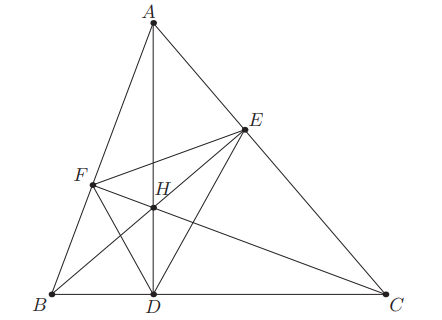
\includegraphics[width=0.5\linewidth]{Figure 1.3A.png}
\end{center}
\end{problem}
We will show the necessary result for one of them ($\triangle AEF$), as it easily generalizes. Clearly, we know that $\triangle ABC$ and $\triangle AEF$ share $\angle A$. In addition, 
\begin{align*}
\angle B &= 90-\angle BAD \\
&= \angle AHF \\
&= \angle AEF.
\end{align*}
Thus, we know that two of the angles are equal, so \[\triangle ABC \sim \triangle AEF\] as required. $\square$

\begin{problem}[1.17]{}
Let $H$ be the orthocenter of $\triangle ABC$, as in the diagram below. Let $X$ be the reflection of $H$ over $\ol{BC}$ and $Y$ the reflection over the midpoint of $\ol{BC}$.
\begin{enumerate}[label=(\alph*)]
    \item Show that $X$ lies on $(ABC)$.
    \item Show that $\ol{AY}$ is a diameter of $(ABC)$.
\end{enumerate}

\begin{center}
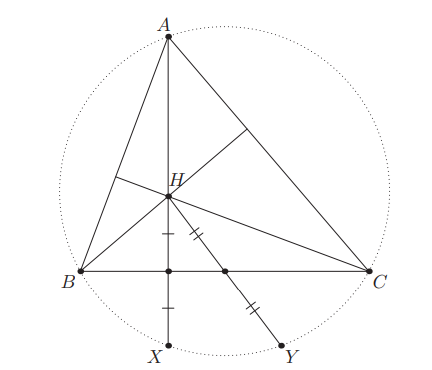
\includegraphics[width=0.35\linewidth]{Figure 1.3B.png}
\end{center}
\end{problem}
We start with part (a). Let the foot of the altitude from $A$ be $D$, from $B$ be $E$, and the foot from $C$ be $F$. Then, we can write the following equations:
\begin{align*}
\angle A + \angle BXC &= \angle A + \angle BHC \\
&= \angle A + \angle FHE \\
&= 180
\end{align*}
so $ABXC$ is cyclic, implying that $X$ lies on $(ABC)$ as desired. 

We proceed with part (b). Define $M$ to be the midpoint of $\ol{BC}$. Then, we know that \[\triangle HDM \sim \triangle HXY.\] This means that \[\angle HXY = \angle AXY = 90.\] Next, we show that $Y$ lies on $(ABC)$, by showing that $AXYC$ is cyclic. We can say that:
\begin{align*}
\angle BCY + \angle C &= \angle HBC + \angle C \\
&= 90
\end{align*}
where $\angle BCY = \angle HBC$ since $\triangle HBM \cong YCM$. This, in conjuction with the fact that $\angle AXY = 90$ means that $AXYC$ is cyclic. So, $Y$ lies on $(ABC)$ as desired. Finally, this means that $\ol{AY}$ is the diameter of $(AXY)$ or equivalently $(ABC)$, as required. $\square$

\begin{remark*}
The complex number proof can be found as \refproblem{6.14}.
\end{remark*}

\begin{problem}[1.28]{}
We claimed that $\dangle FKD + \dangle DKE + \dangle EKF = 0$ in the above proof. Verify this.
\end{problem}
Let $P$ be a point that is collinear with $D$ and $K$. Then, we know that \[\dangle DKE + \dangle EKP = 0\] and \[\dangle PKF + \dangle FKD = 0.\] Adding these gives the desired conclusion. $\square$

\begin{remark*}
Throughout this text, we will use $\dangle$ to denote directed angles.
\end{remark*}

\begin{problem}[1.29]{}
Show that for any distinct points $A$, $B$, $C$, $D$ we have $\dangle ABC + \dangle BCD + \dangle CDA + \dangle DAB = 0$.
\end{problem}
We know that:
\begin{align*}
\dangle BAD + \dangle ADB + \dangle DBA &= 0 \\
\dangle BDC + \dangle DCB + \dangle CBD &= 0.
\end{align*}
Adding these gives that \[\dangle BAD + (\dangle ADB +\dangle BDC) + (\dangle DBA + \dangle CBD) + \dangle DCB  = 0\] and simplifying, we have that \[\dangle BAD + \dangle ADC + \dangle CBA + \dangle DCB = 0.\] Finally, negating the entire equation gives the desired conclusion. $\square$

\begin{problem}[1.30]{}
Points $A$, $B$, $C$ lie on a circle with center $O$. Show that $\dangle OAC = 90^\circ - \dangle CBA$.
\end{problem}
Let $A'$ be the reflection of $A$ across $O$. Then, we know that since $AA'$ is a diameter, \[\dangle ACA' = 90^\circ.\] This implies the following:
\begin{align*}
\dangle ABC &= \dangle AA'C \\
&= -\dangle A'CA - \dangle CAA' \\
&= 90 + \dangle A'AC \\
&= 90 + \dangle OAC.
\end{align*}
This implies that \[\dangle OAC = 90+\dangle ABC\] as desired. $\square$

\newpage

\begin{problem}[1.33]{}
Let $ABC$ be a triangle and let ray $AO$ meet $\ol{BC}$ at $D$. Point $K$ is selected so that $\ol{KA}$ is tangent to $(ABC)$ and $\angle KCB = 90^\circ$. Prove that $\ol{KD} \parallel \ol{AB}$.
\end{problem}
\begin{center}
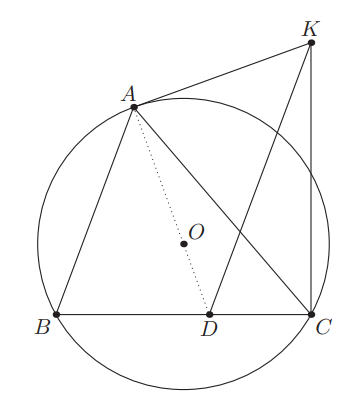
\includegraphics[width=0.4\linewidth]{Figure 1.6B.png}
\end{center}
Since \[\angle KAD = \angle KCD = 90^\circ\] we know that quadrilateral $KADC$ is cyclic. Because of this, we can write that:
\begin{align*}
\angle KDB &= 180-\angle KDC \\
&= 180-\angle KAC \\
&= 180-\angle B
\end{align*}
which implies that $\ol{KD} \parallel \ol{AB}$, as required. $\square$

\begin{problem}[1.34]{}
In scalene triangle $ABC$, let $K$ be the intersection of the angle bisector of $\angle A$ and the perpendicular bisector of $\ol{BC}$. Prove that the points $A$, $B$, $C$, $K$ are concyclic.
\end{problem}

Let $K'$ be the intersection of the angle bisector of $\angle A$ and $(ABC)$ not at $A$. We wish to show that $K' = K$. By the Incenter-Excenter Lemma, we know that \[K'B = K'C\] implying that $K'$ lies on the perpendicular bisector of $\ol{BC}$. Hence, $K'$ is the same point as $K$, and since $ABK'C$ is cyclic, we have the required result. $\square$

\begin{problem}[1.36]{}
Let $ABCDE$ be a convex pentagon such that $BCDE$ is a square with center $O$ and $\angle A = 90^\circ$. Prove that $\ol{AO}$ bisects $\angle BAE$.
\end{problem}
Clearly, $ABOE$ is cyclic since $\angle BOE = 90^\circ$. This means that \[\angle BAO = \angle BEO = 45^\circ.\] So, $\ol{AO}$ bisects $\angle BAE$ as desired. $\square$

\begin{problem}[1.37]{BAMO 1999/2}
Let $O = (0, 0)$, $A = (0, a)$, and $B = (0, b)$, where $0<a<b$ are reals. Let $\Gamma$ be a circle with diameter $\ol{AB}$ and let $P$ be any other point on $\Gamma$. Line $\ol{PA}$ meets the x-axis again at $Q$. Prove that $\angle BQP = \angle BOP$.
\end{problem}
We wish to show that quadrilateral $BPOQ$ is cyclic. We can write the following:
\begin{align*}
\dangle PQO &= \dangle AQO \\
&= 90-\dangle OAQ \\
&= 90-\dangle BAP \\
&= \dangle PBA \\
&= \dangle PBO
\end{align*}
so $BPOQ$ is indeed cyclic. This implies that \[\dangle BQP = \dangle BOP\] as desired. $\square$

\begin{problem}[1.38]{}
In cyclic quadrilateral $ABCD$, let $I_1$ and $I_2$ denote the incenters of $ABC$ and $DBC$, respectively. Prove that $I_1I_2BC$ is cyclic.
\end{problem}
\begin{center}
\begin{asy}
size(6cm);
pair A, B, C, D;
real r = 3;
pair O = (0,0);
A = dir(120)*r;
B = dir(200)*r;
C = dir(340)*r;
D = dir(60)*r;
draw(circle(O,r), gray);
draw(A--B--C--D--cycle, dashed+gray);
dot("$A$", A, dir(120));
dot("$B$", B, dir(200));
dot("$C$", C, dir(340));
dot("$D$", D, dir(60));
pair incenter(pair X, pair Y, pair Z) {
  real a=abs(Y-Z), b=abs(Z-X), c=abs(X-Y);
  return (a*X + b*Y + c*Z)/(a+b+c);
}
pair I1 = incenter(A,B,C);
pair I2 = incenter(D,B,C);
draw(A--B--C--cycle, blue);
draw(D--B--C--cycle, red);
dot("$I_1$", I1, dir(90));
dot("$I_2$", I2, dir(90));
draw(I1--I2--C--B--cycle, heavygreen);
draw(circumcircle(I1,I2,B), dashed+purple);
draw(incircle(A,B,C), gray+dashed);
draw(incircle(D,B,C), gray+dashed);
\end{asy}
\end{center}

Firstly, since $ABCD$ is cyclic, we know that \[\angle BAC = \angle BDC.\] Dividing by two and adding $90$, we get that $90+\frac{\angle BAC}{2} = 90+\frac{\angle BDC}{2}$, which is equivalent to \[\angle BI_1C = \angle BI_2C\] so $BI_1I_2C$ is cyclic, as desired. $\square$

\begin{problem}[1.39]{CGMO 2012/5}
Let $ABC$ be a triangle. The incircle of $\triangle ABC$ is tangent to $\ol{AB}$ and $\ol{AC}$ at $D$ and $E$ respectively. Let $O$ denote the circumcenter of $\triangle BCI$. Prove that $\angle ODB = \angle OEC$.
\end{problem}

\begin{center}
\begin{asy}
import geometry;
size(6cm);
pair A = (0,0);
pair B = (6,0);
pair C = (2,5);
real a = length(B - C);
real b = length(C - A);
real c = length(A - B);
pair I = (a*A + b*B + c*C) / (a + b + c);
real s = (a + b + c)/2;
real area = sqrt(s * (s - a) * (s - b) * (s - c));
real r = area / s;
path incircle = circle(I, r);
pair foot(pair P, pair X, pair Y) {
  pair v = Y - X;
  return X + v * dot(P - X, v) / length(v)^2;
}
pair D = foot(I, A, B);
pair E = foot(I, A, C);
pair O = circumcenter(B, C, I);
draw(A--B--C--cycle, black);
draw(incircle, blue);
draw(circumcircle(B, C, I), dashed + gray);
dot("$A$", A, SW);
dot("$B$", B, SE);
dot("$C$", C, N);
dot("$I$", I, dir(180));
dot("$D$", D, S);
dot("$E$", E, NE);
dot("$O$", O, dir(90));
draw(O--D, red);
draw(D--B, red);
draw(O--E, red);
draw(E--C, red);
draw(I--D, gray + dotted);
draw(I--E, gray + dotted);
\end{asy}
\end{center}

We know that $AEID$ is cyclic since \[\angle AEI + \angle ADI = 180^\circ.\] In addition, we know that $\ol{AI}$ bisects $\angle EID$, and since $A$, $I$, and $O$ are collinear (by the Incenter-Excenter Lemma), we know that $\angle EIO = \angle DIO.$ This implies that \[\triangle EIO \sim \triangle DIO\] since $DI = EI$, which means that \[\angle IEO = \angle IDO.\] Finally, this implies that $\angle ADO = \angle AEO$, which result in the desired claim after negating and adding $180$. $\square$

\begin{problem}[1.40]{Canada 1991/3}
Let $P$ be a point inside circle $\omega$. Consider the set of chords of $\omega$ that contain $P$. Prove that their midpoints all lie on a circle. 
\end{problem}
We claim that all the midpoints lie on the circle with diameter $\ol{OP}$.

Let $M$ be any one of these midpoints. We must show that $\angle OMP = 90^\circ$ for any $M$. Let $A$ be one endpoint of the chord, and $B$, the other. Then, we know that \[\triangle OMA \sim \triangle OMB\] since all the corresponding sides are equal ($OA = OB$ as well). Thus, this means that \[\angle OMA = \angle OMB = 90^\circ\] as desired. $\square$

\begin{remark*}
Note that there are a few exceptions. If $O = M$, then obviously $M$ lies on the circle with diameter $\ol{OP}$. Similarly, if $P = M$, then $M$ obviously lies on that circle.
\end{remark*}

\begin{problem}[1.41]{Russian Olympiad 1996}
Points $E$ and $F$ are on side $\ol{BC}$ of convex quadrilateral $ABCD$ (with $E$ closer than $F$ to $B$). It is known that $\angle BAE$ = $\angle CDF$ and $\angle EAF = \angle FDE$. Prove that $\angle FAC = \angle EDB$.
\end{problem}

\begin{center}
\begin{asy}
size(10cm);
pair A = (0,4);
pair B = (0,0);
pair C = (5,0);
pair D = (4,3);
pair E = B + 0.3*(C - B);
pair F = B + 0.6*(C - B);
draw(A--B--C--D--cycle, linewidth(0.8));
dot("$A$", A, N);
dot("$B$", B, SW);
dot("$C$", C, SE);
dot("$D$", D, NE);
dot("$E$", E, S);
dot("$F$", F, S);
draw(A--E, dashed);
draw(A--F, dashed);
draw(D--E, dashed);
draw(D--F, dashed);
draw(A--C, dotted);
draw(D--B, dotted);
markangle(B,A,E, radius=15);
markangle(F,D,C, radius=15);
markangle(E,A,F, radius=25, n=2);
markangle(E,D,F, radius=25, n=2);
\end{asy}
\end{center}

Clearly, quadrilateral $ADEF$ is cyclic. Thus, we can write the following:
\begin{align*}
\angle D &= \angle ADF + \angle FDC \\
&= 180-\angle AEF+\angle FDC \\
&= \angle AEB + \angle FDC \\
&= 180-\angle BAE - \angle B + \angle FDC \\
&= 180-\angle B.
\end{align*}
Thus, $ABCD$ is cyclic. This implies that \[\angle BAC = \angle CDB\] which implies that \[\angle FAC = \angle EDB\] due to the congruent angles. $\square$

\newpage

\begin{problem}[1.42]{}
Let $ABC$ be an acute triangle inscribed in circle $\Omega$. Let $X$ be the midpoint of the arc $\arc{BC}$ not containing $A$ and define $Y$, $Z$ similarly. Show that the orthocenter of $\triangle XYZ$ is the incenter $I$ of $\triangle ABC$.
\end{problem}
\begin{center}
\begin{asy}
size(6cm);
pair A = dir(110);
pair B = dir(210);
pair C = dir(330);
pair O = (0,0);
pair X = dir((degrees(B)+degrees(C))/2);
pair Y = -dir((degrees(C)+degrees(A))/2);
pair Z = dir((degrees(A)+degrees(B))/2);
pair I = incenter(A,B,C);
pair foot(pair P, pair A, pair B)
{
  pair v = B - A;
  return A + v * dot(P - A, v)/dot(v,v);
}
draw(unitcircle, gray);
draw(A--B--C--cycle, black+1);
draw(X--Y--Z--cycle, blue);
draw(X--foot(X,Y,Z), dashed+red);
draw(Y--foot(Y,Z,X), dashed+red);
draw(Z--foot(Z,X,Y), dashed+red);
dot("$A$", A, dir(90));
dot("$B$", B, dir(210));
dot("$C$", C, dir(330));
dot("$X$", X, dir(X));
dot("$Y$", Y, dir(Y));
dot("$Z$", Z, dir(Z));
dot("$I$", I, dir(270));
dot(I, red+1.5);
\end{asy}
\end{center}
We will show that $\ol{XI} \perp \ol{YZ}$ since the result easily generalizes to the other sides. By the Incenter-Excenter Lemma, we know that $A$, $I$, and $X$ are collinear, and similarly for the other points. This means that:
\begin{align*}
\angle ZXI &= \angle ZXA \\
&= \angle ZCA \\
&= \dfrac{\angle C}{2}.
\end{align*}
On the other hand,
\begin{align*}
\angle Z &= \frac{m\arc{XY}}{2} \\
&= 90-\frac{m\arc{AB}}{4} \\
&= 90-\frac{\angle C}{2}.
\end{align*}
Thus, we get that $\ol{IX} \perp \ol{YZ}$ as required. $\square$

\newpage

\begin{problem}[1.43]{JMO 2011/5}
Points $A$, $B$, $C$, $D$, $E$ lie on a circle $\omega$ and point $P$ lies outside the circle. The given points are such that:
\begin{enumerate}[label={(\roman*)}]
    \item  lines $PB$ and $PD$ are tangent to $\omega$
    \item  $P$, $A$, $C$ are collinear
    \item  $\ol{DE} \parallel \ol{AC}$
\end{enumerate}
Prove that $\ol{BE}$ bisects $\ol{AC}$. 
\end{problem}
\begin{center}
\begin{asy}
size(6cm);
pair A,B,C,D,M,O,P,E; A = dir(130); B = dir(52.5); E = dir(200); D = dir(300); C = dir(10); M = (A+C)/2; O = (0,0); P = (1.8,-0.12);

dot("$A$",A,dir(A)); dot("$B$",B,dir(B)); dot("$C$",C,dir(C)); dot("$D$",D,dir(D)); dot("$E$",E,dir(E)); dot("$M$",M,dir(100)); dot("$P$",P,dir(P)); dot("$O$",O,NE);

draw(unitcircle); draw(A--C); draw(E--D); draw(P--D); draw(P--B); draw(E--B); draw(A--P); draw(A--B--C--D--cycle, dashed);
\end{asy}
\end{center}
Let $O$ be the center of $\omega$. Since $\ol{DE} \parallel \ol{AC}$, we have that \[m\arc{AE} = m\arc{CD}.\] Then, we know that:
\begin{align*}
\angle BMP &= \angle BMC \\
&= \dfrac{m\arc{AE}}{2}+\dfrac{m\arc{BC}}{2} \\
&= \dfrac{m\arc{CD}}{2}+\dfrac{m\arc{BC}}{2} \\
&= \dfrac{m\arc{BD}}{2} \\
&= \angle BOP.
\end{align*}
Thus, quadrilateral $POMB$ is cyclic. Thus, we have that \[\angle OMC = \angle OMP = \angle OBP = 90^\circ\] so $M$ is the midpoint of $\ol{AC}$, as required. $\square$

\newpage

\begin{problem}[1.44]{Three Tangents}
Let $ABC$ be an acute triangle. Let $\ol{BE}$ and $\ol{CF}$ be altitudes of $\triangle ABC$, and denote by $M$ the midpoint of $\ol{BC}$. Prove that $\ol{ME}$, $\ol{MF}$, and the
line through $A$ parallel to $\ol{BC}$ are all tangents to $(AEF)$.
\end{problem}
\begin{center}
\begin{asy}
size(6cm);
defaultpen(fontsize(10pt));
pair A = dir(110);
pair B = dir(210);
pair C = dir(330);
pair E = foot(B, A, C);
pair F = foot(C, A, B);
pair M = (B + C)/2;
pair foot(pair P, pair A, pair B)
{
  pair v = B - A;
  return A + v * dot(P - A, v)/dot(v,v);
}
pair O;
real R;
{
  pair midAE = (A + E)/2;
  pair vAE = E - A;
  pair perpAE = rotate(90)*vAE;

  pair midAF = (A + F)/2;
  pair vAF = F - A;
  pair perpAF = rotate(90)*vAF;

  real t = cross(midAF - midAE, perpAF) / cross(perpAE, perpAF);
  O = midAE + t * perpAE;
  R = length(O - A);
}
pair dirBC = C - B;
pair Q = A + dirBC;
draw(A--B--C--cycle, black+1);
draw(B--E, gray);
draw(C--F, gray);
draw(circle(O,R), deepblue);
draw(M--E, red+dashed);
draw(M--F, red+dashed);
pair v = (C - B)/3;
draw(A - v -- A + v, dashed+blue);
dot("$A$", A, dir(90));
dot("$B$", B, dir(210));
dot("$C$", C, dir(330));
dot("$E$", E, dir(E));
dot("$F$", F, dir(F));
dot("$M$", M, dir(270));
pair intersect(pair A, pair v, pair B, pair w)
{
  real t = cross(B - A, w) / cross(v, w);
  return A + t * v;
}
pair H = intersect(B, E - B, C, F - C);
dot("$H$", H, dir(270));
\end{asy}
\end{center}
We will show that $\ol{ME}$ is tangent, and $\ol{MF}$ can be derived easily using a similar method. We know that \[\angle HAE = 90-\angle C.\] In addition, since $\triangle BEC$ is a right triangle, and $\ol{EM}$ is the median, we know that $\triangle BME$ is isosceles, and so \[\angle MEB = \angle MBE = 90-\angle C.\] So \[\angle HAE = \angle MEB = \angle MEH\] implying that $\ol{ME}$ is tangent to $(AEF)$. The proof for $\ol{MF}$ is similar, so we omit it. Now let $P$ be a point on $\ol{BC}$ on the side of $B$. Then, we have that \[\angle FAP = \angle B\] due to parallel lines. In addition, we can say that \[\angle AHF = 90-\angle HAF = \angle B.\] So, we have that \[\angle FAP = \angle AHF\] implying that $\ol{AP}$ is tangent to $(AEF)$, as desired. $\square$

\newpage

\begin{problem}[1.45]{Right Angles on Incircle Chord}
The incircle of $\triangle ABC$ is tangent to $\ol{BC}$, $\ol{CA}$, $\ol{AB}$ at $D$, $E$, $F$, respectively. Let $M$ and $N$ be the midpoints of $\ol{BC}$ and $\ol{AC}$, respectively. Ray $BI$ meets line $EF$ at $K$.
\begin{enumerate}[label={(\roman*)}]
    \item  Show that $\ol{BK} \perp \ol{CK}$.
    \item  Show $K$ lies on line $MN$.
\end{enumerate}
\end{problem}
\begin{center}
\begin{asy}
size(6cm);
defaultpen(fontsize(10pt));
pair foot(pair P, pair A, pair B) {
  pair v = B - A;
  return A + v * dot(P - A, v)/dot(v,v);
}
pair intersect(pair A, pair v, pair B, pair w) {
  real t = cross(B - A, w)/cross(v, w);
  return A + t*v;
}
pair A = (-1,3);
pair B = (-2,0);
pair C = (2,0);
real a = length(B - C);
real b = length(C - A);
real c = length(A - B);
real s = (a+b+c)/2;
pair I = (a*A + b*B + c*C) / (a+b+c);
real r = sqrt((s - a)*(s - b)*(s - c)/s);
pair D = foot(I, B, C);
pair E = foot(I, C, A);
pair F = foot(I, A, B);
pair M = (B+C)/2;
pair N = (A+C)/2;
pair dirEF = F - E;
pair dirBI = I - B;
pair K = intersect(B, dirBI, E, dirEF);
draw(A--B--C--cycle, black+1);
draw(circle(I,r), deepblue);
draw(K--F, dashed+blue);
draw(B--K, dashed+red);
draw(B--K, red);
draw(C--K, red);
draw(M--N, purple);
draw(N--K, dashed+purple);
dot("$A$", A, dir(90));
dot("$B$", B, dir(225));
dot("$C$", C, dir(315));
dot("$I$", I, dir(90));
dot("$D$", D, dir(270));
dot("$E$", E, dir(E));
dot("$F$", F, dir(F));
dot("$M$", M, dir(270));
dot("$N$", N, dir(45));
dot("$K$", K, dir(45));
\end{asy}
\end{center}

We start with the first part. Clearly, we know that $\triangle BMK$ is isosceles. This implies that \[\angle BKM = \dfrac{\angle B}{2}.\] In addition, this also implies that $\triangle KMC$ is isosceles. So, we know that \[\angle MKC = 90-\dfrac{\angle KMC}{2} = \dfrac{\angle BMK}{2} = 90-\dfrac{\angle B}{2}.\] Thus, we know that $\angle BKC$ is right, as required.

We proceed with the second part. All we must show is that \[\angle KMC = \angle NMC = \angle B.\] We already established that $\triangle KMC$ is isosceles. Hence, we know that \[\angle KMC = 180-2\angle MKC = \angle B\] as required. $\square$

\newpage

\begin{problem}[1.46]{Canada 1997/4}
The point $O$ is situated inside the parallelogram $ABCD$ such that $\angle AOB + \angle COD = 180^\circ$. Prove that $\angle OBC = \angle ODC$.
\end{problem}
\begin{center}
\begin{asy}
size(6cm);
defaultpen(fontsize(10pt));
pair A = (0,0);
pair B = (4,0);
pair C = B + (1,3);
pair D = A + (1,3);
pair O = (2,1.2);
pair O_shifted = O + (A - D);
draw(A--B--C--D--cycle, black+1);
draw(A--C, gray+dashed);
draw(O--A, blue);
draw(O--B, blue);
draw(O--C, blue);
draw(O--D, blue);
draw(O--O_shifted, red);
draw(A--O_shifted, dotted);
draw(B--O_shifted, dotted);
dot("$A$", A, SW);
dot("$B$", B, SE);
dot("$C$", C, NE);
dot("$D$", D, NW);
dot("$O$", O, dir(90));
dot("$O'$", O_shifted, dir(270));
\end{asy}
\end{center}

Let $O'$ be defined as the translation of $O$ using the vector $\ray{DA}$ (or equivalently $\ray{CB}$). Now, we can write that
\begin{align*}
\triangle DOA &\cong \triangle O'AO \\
\triangle COB &\cong \triangle O'BO
\end{align*}
because of the parallelograms created. Because of this, we can write that
\begin{align*}
\angle AO'B &= \angle AO'O + \angle BO'O \\
&= \angle ADO + \angle BCO \\
&= 180 - \angle ODC - \angle OCD \\
&= \angle DOC \\
&= 180-\angle AOB
\end{align*}
so quadrilateral $AO'BO$ is cyclic. Finally, we can say that:
\begin{align*}
\angle OBA &= \angle OO'A \\
&= \angle ODA
\end{align*}
and since $\angle B = \angle D$ this implies that \[\angle OBC = \angle OBA\] as required. $\square$

\newpage

\begin{problem}[1.47]{IMO 2006/1}
Let $ABC$ be a triangle with incenter $I$. A point $P$ in the interior of the triangle satisfies $\angle PBA+\angle PCA=\angle PBC+\angle PCB$. Show that $AP \ge AI$ and that equality holds if and only if $P = I$.
\end{problem}
\begin{center}
\begin{asy}
size(6cm);
defaultpen(fontsize(10pt));
pair A = (-1,3);
pair B = (-2,0);
pair C = (2,0);
real a = length(B - C);
real b = length(C - A);
real c = length(A - B);
pair I = (a*A + b*B + c*C)/(a + b + c);
pair P = (0.3,1.1);
draw(A--B--C--cycle, black+1);
draw(A--I, deepgreen+1.2);
draw(B--I, dotted);
draw(C--I, dotted);
draw(A--P, orange+1.2+dashed);
draw(P--B, black+dashed);
draw(P--C, black+dashed);
dot("$A$", A, dir(90));
dot("$B$", B, SW);
dot("$C$", C, SE);
dot("$I$", I, dir(180));
dot("$P$", P, dir(270));
\end{asy}
\end{center}
We can rewrite the condition as \[\angle PBA+\angle PCA = \angle B - \angle PBA + \angle C - \angle PCA\] which simplifies to \[\angle PBA + \angle PCA = \frac{\angle B}{2}+\frac{\angle C}{2}.\] We can rearrange this to \[\angle PBA - \frac{\angle B}{2} = \frac{\angle C}{2}-\angle PCA.\] This implies that $P$ must lie on $(BIC)$. 

It is well known that the minimum distance from any point to a circle can be found by finding the distance from that point to intersection of the segment with endpoints of the center of the circle and that point. In addition, by the Incenter-Excenter Lemma, we know that $A$, $I$ and the center of $(BIC)$ are collinear, so the minimum distance from $A$ to $(BIC)$ is $AI$. Hence, we must have \[AP \ge AI\] for any $P$, with equality that holds if and only if $P = I$, as required. $\square$

\begin{problem}[1.48]{Simson Line}
Let $ABC$ be a triangle and $P$ be any point on $(ABC)$. Let $X$, $Y$, $Z$ be the feet of the perpendiculars from $P$ onto lines $BC$, $CA$, and $AB$. Prove that points $X$, $Y$, $Z$ are collinear.
\end{problem}
It suffices to show that \[\dangle PYX = \dangle PYZ.\] We can establish that $PYXC$ is cyclic since \[\dangle PYC = \dangle PXC = 90^\circ.\] Similarly, we know that $PZAY$ is cyclic since \[\dangle PYA = \dangle PZA = 90^\circ.\] Then, we can say that 
\begin{align*}
\dangle PYX &= \dangle PCX \\
&= \dangle PCB \\
&= \dangle PAB \\
&= \dangle PAZ \\
&= \dangle PYZ
\end{align*}
where the third line follows because $PABC$ is cyclic. This is the desired conclusion. $\square$

\begin{remark*}
A proof by complex numbers can be found as part (a) of \refproblem{6.22}.
\end{remark*}

\begin{problem}[1.49]{USAMO 2010/1}
Let $AXYZB$ be a convex pentagon inscribed in a semicircle of diameter $\ol{AB}$. Denote by $P$, $Q$, $R$, $S$ the feet of the perpendiculars from $Y$ onto lines $AX$, $BX$, $AZ$, $BZ$, respectively. Prove that the acute angle formed by lines $PQ$ and $RS$ is half the size of $\angle XOZ$, where $O$ is the midpoint of segment $\ol{AB}$.
\end{problem}
\begin{center}
\begin{asy}
import geometry;
size(10cm);
pair A = (-4,0), B = (4,0), O = (0,0);
path semicirc = arc(O,4,0,180);
draw(semicirc);
draw(A--B, gray);

pair X = 4*dir(135);
pair Y = 4*dir(80);
pair Z = 4*dir(30);

draw(A--X--Y--Z--B--cycle, blue+linewidth(1));

pair P = foot(Y, A, X);
pair Q = foot(Y, B, X);
pair R = foot(Y, A, Z);
pair S = foot(Y, B, Z);
pair T = intersectionpoint(line(P,Q), line(R,S));

dot(T, blue);

draw(Y--P, gray+dotted);
draw(Y--Q, gray+dotted);
draw(Y--R, gray+dotted);
draw(Y--S, gray+dotted);
draw(X--P, gray+dashed);
draw(B--X, gray+dashed);
draw(A--Z, gray+dashed);
draw(Z--S, gray+dashed);

draw(P--Q, red+linewidth(1.2));
draw(R--S, red+linewidth(1.2));

draw(O--X, dashed+gray);
draw(O--Z, dashed+gray);

draw(Q--T, red+dashed);
draw(R--T, red+dashed);

label("$A$", A, SW);
label("$B$", B, SE);
label("$O$", O, dir(270));
label("$X$", X, dir(X));
label("$Y$", Y, dir(Y));
label("$Z$", Z, dir(Z));
label("$P$", P, dir(P-Y));
label("$Q$", Q, dir(Q-Y));
label("$R$", R, dir(R-Y));
label("$S$", S, dir(S-Y));
label("$T$", T, dir(270));
\end{asy}
\end{center}
Let $T$ be the intersection between lines $PQ$ and $RS$. Notice that we can write $\angle QTR$ as 
\begin{align*}
\angle QTR &= \angle PQY - \angle QYT + \angle SRY - \angle RYT \\
&= \angle PQY + \angle SRY - \angle QYR \\
&= \angle PXY + \angle SZY - \angle QYR \\
&= 180 - \angle AXY + 180 - \angle YZB - \angle ZAB - \angle XBA \\
&= \angle ABY + \angle YAB - \angle ZAB - \angle XBA \\
&= \angle XBY + \angle YAZ \\
&= \dfrac{\angle XOZ}{2}
\end{align*}
as required. $\square$

\newpage

\begin{problem}[1.50]{IMO 2013/4}
Let $ABC$ be an acute triangle with orthocenter $H$, and let $W$ be a point on the side $\ol{BC}$, between $B$ and $C$. The points $M$ and $N$ are the feet of the altitudes drawn from $B$ and $C$, respectively. $\omega_1$ is the circumcircle of triangle $BWN$ and $X$ is a point such that $\ol{WX}$ is a diameter of $\omega_1$. Similarly, $\omega_2$ is the circumcircle of triangle $CWM$ and $Y$ is a point such that $\ol{WY}$ is a diameter of $\omega_2$. Show that the points $X$, $Y$, and $H$ are collinear.
\end{problem}
\begin{center}
\begin{asy}
size(10cm);

pair A = dir(110);
pair B = dir(210);
pair C = dir(330);
pair H = orthocenter(A,B,C);
pair M = foot(B, A, C);
pair N = foot(C, A, B);
pair W = (5*B + 3*C)/8;

pair O1 = circumcenter(B,W,N);
real r1 = abs(O1 - B);
pair O2 = circumcenter(C,W,M);
real r2 = abs(O2 - C);

pair X = 2*O1 - W;
pair Y = 2*O2 - W;

pair[] inter = intersectionpoints(circle(O1,r1), circle(O2,r2));

pair P;
if (abs(inter[0]-W) < 1e-6)
  P = inter[1];
else
  P = inter[0];

// Draw triangle
draw(A--B--C--cycle, blue);

draw(B--M, dotted+gray);
draw(C--N, dotted+gray);

draw(B--C);

pair O3 = circumcenter(A,H,P);
real r3 = abs(O3 - A);

draw(circle(O1, r1), orange);
draw(circle(O2, r2), purple);
draw(circle(O3, r3), gray+dashed);

draw(W--X, orange+linewidth(1));
draw(W--Y, purple+linewidth(1));

draw(H--X, dashed+red);
draw(H--Y, dashed+red);

draw(A--P, gray);

dot(A); dot(B); dot(C); dot(H); dot(W);
dot(M); dot(N);
dot(X, blue);
dot(Y, blue);
dot(P, red);

label("$A$", A, dir(90));
label("$B$", B, SW);
label("$C$", C, SE);
label("$H$", H, dir(140));
label("$W$", W, dir(-90));
label("$M$", M, dir(M));
label("$N$", N, dir(N));
label("$X$", X, dir(X));
label("$Y$", Y, dir(Y));
label("$P$", P, dir(NE));
\end{asy}
\end{center}

Let $P$ be the second intersection between the two circumcircles (other than $W$). We will show that $X$, $H$, and $P$ are collinear, and the same result can easily be replicated for $Y$. First, note that by the Miquel Point, $ANPM$ is cyclic, and because \[\angle ANH = \angle AMH = 90^\circ\] $ANHM$ is also cyclic. This implies that pentagon $ANHPM$ is cyclic. Next, we prove that $A$, $P$, and $W$ are collinear. This is equivalent to show that \[\angle APM + \angle WPM = 180^\circ.\] We can do this as follows:
\begin{align*}
\angle APM &= \angle AHM \\
&= 90-\angle HAM \\
&= \angle C \\
&= 180-\angle WPM
\end{align*}
as required. Now, we can say that \[\angle APH = \angle XPW = 90^\circ\] so $X$, $H$, and $P$ are collinear. We repeat this with $Y$ to get a similar result, which implies that $X$, $H$, and $Y$ are collinear, as required. $\square$

\begin{problem}[1.51]{IMO 1985/1}
A circle has center on the side $\ol{AB}$ of the cyclic quadrilateral $ABCD$. The other three sides are tangent to the circle. Prove that $AD + BC = AB$.
\end{problem}
\begin{center}
\begin{asy}
size(10cm);
import graph;

pair O = (0,0);
real R = 4;
draw(circle(O,R), deepcyan);

pair A = R*dir(168.5);
pair B = R*dir(11.5);
pair D = R*dir(110);
pair C = reflect(O, A+B)*(D);

draw(A--B--C--D--cycle, blue+linewidth(1));

pair O2 = (A + B)/2;
real r = 2.93;
draw(circle(O2, r), orange);

dot("$A$", A, dir(150));
dot("$B$", B, dir(30));
dot("$C$", C, dir(C));
dot("$D$", D, dir(D));
dot("$O$", O, dir(90));
dot("$O'$", O2, dir(60));
dot("$P$", O2-(0.1, 0), dir(270));
\end{asy}
\end{center}
Let $P$ be the point on $\ol{AB}$ such that \[AD = AP.\] We wish to show that \[BC = BP.\] We can first notice that $DPO'C$ is cyclic since
\begin{align*}
\angle DPO' &= 180-\angle DPA \\
&= 90+\dfrac{\angle DAP}{2} \\
&= 90+\dfrac{180-\angle C}{2} \\
&= 180-\angle DCO'.
\end{align*}
Next, we will show that $\triangle PBC$ is isosceles. We can say that: 
\begin{align*}
\angle CPB &= \angle CPO' \\
&= \angle CDO' \\
&= \dfrac{\angle D}{2} \\
&= 90-\dfrac{\angle B}{2}
\end{align*}
so $\triangle PBC$ is indeed isosceles, implying that \[BP = BC\] as desired. $\square$

\newpage

\section{Circles}

\begin{problem}[2.5]{}
Prove the following (Theorem 2.3): Consider a circle $\omega$ and an arbitrary point $P$. 
\begin{enumerate}[label=(\alph*)]
\item The quantity $\Pow_\omega(P)$ is positive, zero, or negative according to whether $P$ is outside, on, or inside $\omega$, respectively. 
\item If is a line through $P$ intersecting $\omega$ at two distinct points $X$ and $Y$, then \[PX\cdot PY=|\Pow_{\omega}(P)|.\] 
\item If $P$ is outside $\omega$ and $\ol{PA}$ is a tangent to $\omega$ at a point $A$ on $\omega$, then \[PA^2 =\Pow_{\omega}(P).\]
\end{enumerate}
\end{problem}
For completeness, we define $\Pow$.
\begin{definition*}
Let $O$ be the center of $\omega$. We define $\Pow_\omega(P)$ as the quantity $OP^2-r^2$ if $r$ is the radius of $\omega$.
\end{definition*}
We start with part (a). If $P$ is inside $\omega$, then $OP < r$, so $\Pow_\omega(P)$ is negative. If $P$ is on $\omega$, then $OP = r$, so $\Pow_\omega(P)$ is zero. Similarly, if $P$ is outside $\omega$, then $OP > r$, so $\Pow_\omega(P)$ is positive.

We continue with part (b). Let the diameter through $P$ intersect $\omega$ at $A$ and $B$. Then, we know that \[\triangle APX \sim \triangle YPB.\] Then, we know that \[\dfrac{AP}{YP} = \dfrac{PX}{PB}.\] So, we know that \[PX\cdot PY = PA\cdot PB = (OP+r)(OP-r) = \abs{\Pow_{\omega}(P)}\] as required.

We finish with part (c). We already know that \[PA \cdot PB = PX \cdot PY.\] Now, move the line creating $A$ and $B$ closer and closer to the circumference. Consider the limiting case, when $A=B$. In this case, we can write that \[PA^2 = PX\cdot PY = \Pow_\omega(P)\] as required. $\square$

\newpage

\begin{problem}[2.6]{}
Let $ABC$ be a right triangle with $\angle ACB = 90^\circ$. Give a proof of the Pythagorean theorem.
\end{problem}
\begin{center}
\begin{asy}
unitsize(4cm);
draw(unitcircle);
dot("B",(0,0),N);
dot("C",(0,-1),S);
dot("A",(1.4,-1),E);
draw((0,0)--(0,-1)--(1.4,-1)--cycle);
draw((0,-0.95)--(0.05,-0.95)--(0.05,-1));
label("$a$",(0,-0.5),W);
label("$b$",(0.7,-1),S);
label("$c$",(1.1,-0.775),NE);
\end{asy}
\end{center}

Note that by Power of a Point, we have that \[b^2 = c(c+2a).\] Solving this equation yields the following:
\begin{align*}
b^2 &= c^2+2ac \\
a^2+b^2 &= (a+c)^2
\end{align*}
which is equivalent to the Pythagorean Theorem in the given diagram.

\newpage

\begin{problem}[2.11]{}
Let $ABC$ be a triangle and consider a point $P$ in its interior. Suppose that $\ol{BC}$ is tangent to the circumcircles of triangles $ABP$ and $ACP$. Prove that ray $AP$ bisects $\ol{BC}$.
\end{problem}
\begin{center}
\begin{asy}
unitsize(4cm);
pair A = (-0.22,1.6);
pair B = (-1,0);
pair C = (1,0);
pair M = (B + C)/2;
pair P = 0.38*A + 0.62*M;
pair O1 = circumcenter(A,B,P);
pair O2 = circumcenter(A,C,P);
real widen = 15;
real thetaA1 = degrees(dir(A - O1));
real thetaB1 = degrees(dir(B - O1));
real start1 = thetaA1 + widen;
real end1 = thetaB1 - widen;
if (start1 < end1) start1 += 360;
draw(arc(O1, abs(A - O1), start1, end1, CW));
real thetaA2 = degrees(dir(A - O2));
real thetaC2 = degrees(dir(C - O2));
real start2 = thetaA2 - widen;
real end2 = thetaC2 + widen;
if (start2 > end2) end2 += 360;
draw(arc(O2, abs(A - O2), start2, end2, CCW));
draw(A--B--C--cycle);
draw(A--M, dashed);
dot("$A$", A, N);
dot("$B$", B, SW);
dot("$C$", C, SE);
dot("$P$", P, E);
dot("$M$", M, S);
\end{asy}
\end{center}
We know that the midpoint of $\ol{BC}$ (which we call $M$) lies on the radical axis of $(ABP)$ and $(ACP)$ because \[\Pow_{(ABP)}(M)=\Pow_{(ACP)}(M)\] which is due to the fact that the length of the tangents to those circles are equal. $\square$

\begin{problem}[2.12]{}
Show that the orthocenter of a triangle exists using radical axes. That is, if $\ol{AD}$, $\ol{BE}$, and $\ol{CF}$ are altitudes of a triangle $ABC$, show that the altitudes are concurrent.
\end{problem}
Consider the circles with diameters $\ol{AB}$, $\ol{AC}$, and $\ol{BC}$. These circles' common chords (considered pairwise) are the aforementioned altitudes. Thus, since the radical center exists, so does the orthocenter. $\square$

\begin{problem}[2.18]{}
Let the external angle bisectors of $B$ and $C$ in a triangle $ABC$ intersect at $I_A$. Show that $I_A$ is the center of a circle tangent to $\ol{BC}$, the extension of $\ol{AB}$ through $B$, and the extension of $\ol{AC}$ through $C$. Furthermore, show that $I_A$ lies on ray $AI$.
\end{problem}
Clearly, the circle tangent to $\ol{BC}$, the extension of $\ol{AB}$ through $B$, and the extension of $\ol{AC}$ through $C$ exists. Now, since this circle is tangent to $\ol{BC}$ and the the extension of $\ol{AB}$ through $B$, we know that the center lies on the external angle bisector of $B$. Similarly, the center also lies on the external angle bisector of $C$, as desired. Finally, by the Incenter-Excenter Lemma, $A$, $I$, and $I_A$ are collinear. $\square$

\begin{problem}[2.19]{}
Prove that the A-exradius has length \[r_a = \dfrac{s}{s-a}r.\]
\end{problem}
\begin{center}
\begin{asy}
size(10cm);
import geometry;

pair A = (-1,3.5);
pair B = (-2,0);
pair C = (2,0);

real a = length(B - C);
real b = length(C - A);
real c = length(A - B);

pair I = incenter(A,B,C);
real r = inradius(A,B,C);
path incircle = circle(I,r);

pair IA = (-a*A + b*B + c*C)/(-a + b + c);

pair X = foot(IA,B,C);
real R = abs(IA - X);
path excircle = circle(IA,R);

pair D = foot(I,B,C);
pair E = foot(I,A,C);
pair F = foot(I,A,B);

draw(A--B--C--cycle);

draw(incircle);
draw(excircle, dashed);

draw(A--IA, dashed);
draw(IA--B, dashed);
draw(IA--C, dashed);

pair[] bInts = intersectionpoints(excircle, A--B + 10*(B - A));
pair B1 = (abs(bInts[0]-B)>abs(bInts[1]-B)) ? bInts[0] : bInts[1];

pair[] cInts = intersectionpoints(excircle, A--C + 10*(C - A));
pair C1 = (abs(cInts[0]-C)>abs(cInts[1]-C)) ? cInts[0] : cInts[1];

draw(B1--A--C1);

label("$A$",A,dir(90));
label("$B$",B,W);
label("$C$",C,E);
label("$I$",I,NE);
label("$I_A$",IA,S);
label("$D$",D,N);
label("$E$",E,NE);
label("$F$",F,NW);
label("$X$",X,N);
label("$B_1$",B1,W);
label("$C_1$",C1,E);

dot(A);
dot(B);
dot(C);
dot(I);
dot(IA);
dot(D);
dot(E);
dot(F);
dot(X);
dot(B1);
dot(C1);
\end{asy}
\end{center}

Clearly, \[\triangle AFI \sim \triangle AB_1I_A.\] Thus, we have that \[\dfrac{AB_1}{B_1I_A} = \dfrac{AF}{FI} = \dfrac{s-a}{r}.\] So, we know that \[\dfrac{s-a}{r} = \dfrac{AB_1}{B_1I_A} = \dfrac{s}{r_a}\] as required. $\square$

\newpage

\begin{problem}[2.20]{}
Let $ABC$ be a triangle. Suppose its incircle and $A$-excircle are tangent to $\ol{BC}$ at $X$ and $D$, respectively. Show that $BX = CD$ and $BD = CX$.
\end{problem}
Refer to the diagram in Problem 2.19.

We will show the former, and that will imply the latter. We know that:
\begin{align*}
BX &= BB_1 \\
&= AB_1 - AB \\
&= s-c \\
&= DC
\end{align*}
as required. $\square$

\begin{problem}[2.24]{}
Let $ABC$ be a triangle with $I_A$, $I_B$, and $I_C$ as excenters. Prove that triangle $I_AI_BI_C$ has orthocenter $I$ and that triangle $ABC$ is its orthic triangle.
\end{problem}
\begin{center}
\begin{asy}
size(10cm);

pair A = dir(110);
pair B = 1.5*dir(5);
pair C = dir(-130);
real a = length(B - C);
real b = length(C - A);
real c = length(A - B);

pair I = incenter(A,B,C);

pair I_A = (-a*A + b*B + c*C)/(-a + b + c);
pair I_B = (a*A - b*B + c*C)/(a - b + c);
pair I_C = (a*A + b*B - c*C)/(a + b - c);

draw(A--B--C--cycle, black+1);
draw(I_A--I_B--I_C--cycle, blue+1);

dot("$I$", I, dir(90));

dot("$I_A$", I_A, dir(I_A));
dot("$I_B$", I_B, dir(I_B));
dot("$I_C$", I_C, dir(I_C));

pair Ha = foot(I, I_B, I_C);
pair Hb = foot(I, I_C, I_A);
pair Hc = foot(I, I_A, I_B);

dot("$A$", Ha, dir(Ha));
dot("$B$", Hb, dir(Hb));
dot("$C$", Hc, dir(Hc));

draw(I--Ha, dashed+red);
draw(I--Hb, dashed+red);
draw(I--Hc, dashed+red);
draw(I--I_A, dashed+red);
draw(I--I_B, dashed+red);
draw(I--I_C, dashed+red);
\end{asy}
\end{center}

We already know that any vertex is collinear with the incenter and its corresponding excenter (by the Incenter-Excenter Lemma). Thus, all we must prove is that the segment from any vertex to the corresponding excenter is perpendicular to the segment formed by the other two excenters. If we prove that \[\ol{I_BB} \perp \ol{I_AI_C}\] then we can easily generalize this to the other sides.
\begin{align*}
\angle I_BBI_A &= \angle I_BBC + \angle CBI_A \\
&= \angle IBC + \dfrac{180 - \angle B}{2} \\
&= \dfrac{\angle B}{2} + \dfrac{180 - \angle B}{2} \\
&= 90
\end{align*}
as claimed. $\square$

\begin{problem}[2.25]{Pitot's Theorem}
Let $ABCD$ be a quadrilateral. If a circle can be inscribed in it, prove that $AB+CD = BC+DA$.
\end{problem}
We leave many details to the reader, as this proof is relatively elementary. The circle tangent to $ABCD$ will divide up the sides into two parts, each of which will have a corresponding congruent side on the side adjacent to it. Adding up the opposite sides, will then result in equality.

\begin{problem}[2.26]{USAMO 1990/5}
An acute-angled triangle $ABC$ is given in the plane. The circle with diameter $\ol{AB}$ intersects altitude $\ol{CC'}$ and its extension at points $M$ and $N$, and the circle with diameter $\ol{AC}$ intersects altitude $\ol{BB'}$ and its extensions at $P$ and $Q$. Prove that the points $M$, $N$, $P$, $Q$ lie on a common circle.
\end{problem}
\begin{center}
\begin{asy}
import geometry;
unitsize(1cm);

pair A = (2,5);
pair B = (6,0);
pair C = (0,0);
pair H = orthocenter(A,B,C);

pair A_ = extension(A,H,B,C);
pair B_ = extension(B,H,A,C);
pair C_ = extension(C,H,A,B);

pair O = (A + B)/2;
real R = length(A - B)/2;
path circ = circle(O,R);

pair O2 = (A + C)/2;
real R2 = length(A - C)/2;
path circ2 = circle(O2,R2);

// Construct an extended line through C and C'
path longLine = C + 5*(C_ - C) -- C - 5*(C_ - C);

// Intersections
pair[] X = intersectionpoints(circ, longLine);

// M and N
pair M, N;
if (X.length >= 2) {
  M = X[0];
  N = X[1];
} else {
  // Fallback in case tangent
  M = N = X[0];
}

// Construct an extended line through C and C'
path longLine2 = B + 5*(B_ - B) -- B - 5*(B_ - B);

// Intersections
pair[] Y = intersectionpoints(circ2, longLine2);

// M and N
pair P, Q;
if (Y.length >= 2) {
  P = Y[0];
  Q = Y[1];
} else {
  // Fallback in case tangent
  P = Q = Y[0];
}

// Draw triangle
draw(A--B--C--cycle);

// Draw altitudes
draw(A--A_, blue);
draw(B--B_, blue);
draw(C--C_, blue);

draw(C_--M, blue+dotted);
draw(B_--P, blue+dotted);

// Draw circles
draw(circ, dashed+purple);
draw(circ2, dashed+purple);

// Draw points
dot("$A$", A, dir(90));
dot("$B$", B, SE);
dot("$C$", C, SW);
dot("$H$", H, E);
dot("$A'$", A_, S);
dot("$B'$", B_, NW);
dot("$C'$", C_, NE);
dot("$M$", M, dir(M));
dot("$N$", N, dir(270));
dot("$P$", P, dir(180));
dot("$Q$", Q, dir(270));
\end{asy}
\end{center}

Clearly, lines $MN$ and $PQ$ intersect on the radical axis of the two circles ($\ol{AA'}$), since they intersect at $H$. Thus, we know that $M$, $N$, $P$, and $Q$ lie on a common circle by the Radical Center of Intersecting Circles. 

We can write this out if necessary: Let $\omega_1$ be the circle with diameter $\ol{AB}$, and $\omega_2$ the circle with diameter $\ol{AC}$. Then, \[HP \cdot HQ = \Pow_{\omega_2}(H) = \Pow_{\omega_1}(H) = HM \cdot HN\] so $M$, $N$, $P$, and $Q$ are indeed concyclic by the Converse of Power of a Point. $\square$

\begin{problem}[2.27]{BAMO 2012/4}
Given a segment $\ol{AB}$ in the plane, choose on it a point $M$ different from $A$ and $B$. Two equilateral triangles $AMC$ and $BMD$ in the plane are constructed on the same side of segment $\ol{AB}$. The circumcircles of the two triangles intersect in point $M$ and another point $N$. 
\begin{enumerate}[label=(\alph*)]
\item Prove that $\ol{AD}$ and $\ol{BC}$ pass through point $N$. 
\item Prove that no matter where one chooses the point $M$ along segment $\ol{AB}$, all lines $MN$ will pass through some fixed point $K$ in the plane.
\end{enumerate}
\end{problem}
\begin{center}
\begin{asy}
import geometry;
size(10cm);
unitsize(1cm);

pair A = (0, 0);
pair B = (6, 0);
pair M = (2.5, 0);
pair C = rotate(-60, M)*A;
pair D = rotate(60, M)*B;
pair K = rotate(60, B)*A;

path circ1 = circumcircle(A, M, C);
path circ2 = circumcircle(B, M, D);

pair[] X = intersectionpoints(circ1, circ2);

pair N;
if (X.length == 2) {
  N = (X[0] == M) ? X[1] : X[0];
} else {
  N = X[0];
}

draw(A--B, black+1);
draw(A--C--M--cycle, blue);
draw(B--D--M--cycle, blue);
draw(A--K--B, black);

draw(circ1, dashed+blue);
draw(circ2, dashed+blue);

draw(A--D, red);
draw(B--C, red);
draw(M--N, heavygray+1);
draw(M--K, heavygray+1+dotted);
draw(C--D,blue+dotted+1);

dot("$A$", A, SW);
dot("$B$", B, SE);
dot("$M$", M, S);
dot("$C$", C, NW);
dot("$D$", D, NE);
dot("$K$", K, S);
dot("$N$", N, dir(N));
\end{asy}
\end{center}

We start with part (a). Clearly, quadrilaterals $ACNM$ and $BDNM$ are cyclic. Now, we just need to show that $N$ lies on both $\ol{AD}$ and $\ol{BC}$. We can do this as follows:
\begin{align*}
\dangle AND &= \dangle ANM + \dangle MND \\
&= \dangle ACM + \dangle MBD \\
&= 0
\end{align*}
so $N$ lies on $\ol{AD}$. We can do the same for $\ol{BC}$ and get that $N$ lies on $\ol{BC}$ as well, as required.

We proceed with part (b). We wish to show that this point $K$ is the point on the opposite side of $\ol{AB}$ such that $\triangle AKB$ is equilateral. Hence, we can show that line $NM$ always passes through $K$. Now, since $\ol{NM}$ is the radical axis of the two circumcircles, it suffices to show that the tangents to the two circles are always equal in length. 

We start by showing that $\ol{KA}$ is tangent to $(ACM)$. Let the center of $(ACM)$ be $O_1$. Then, we know that:
\begin{align*}
\dangle O_1AK &= \dangle O_1AM + \dangle MAK \\
&= 90.
\end{align*}
We can show something similar for the other circle as well. Thus, $\ol{AK}$ is tangent to $(ACM)$ and $\ol{BK}$ is tangent to $(BDM)$. Finally, since \[AK = BK\] we know that \[\Pow_{(ACM)}(K) = \Pow_{(BDM)}(K).\] So, $K$ lies on line $NM$, as desired. $\square$

\begin{problem}[2.28]{JMO 2012/1}
Given a triangle $ABC$, let $P$ and $Q$ be points on segments $\ol{AB}$ and $\ol{AC}$, respectively, such that $AP = AQ$. Let $S$ and $R$ be distinct points on segment $\ol{BC}$ such that $S$ lies between $B$ and $R$, $\angle BPS = \angle PRS$, and $\angle CQR = \angle QSR$. Prove that $P$, $Q$, $R$, $S$ are concyclic.
\end{problem}
\begin{center}
\begin{asy}
import graph; 
size(10.46cm);
pen dps = linewidth(0.7) + fontsize(10); defaultpen(dps);
pen dotstyle = black;
real xmin = -5.9, xmax = 14.56, ymin = -3.95, ymax = 11.77;
pen zzttqq = rgb(0.6,0.2,0);

pair A = (2.72,5.22);
pair B = (1.18,3.1);
pair C = (5.42,2.82);
pair P = (1.97,4.19);
pair Q = (3.67,4.37);
pair R = (3.9,2.92);
pair S = (1.84,3.06);

draw(A--B--C--cycle, zzttqq);
draw(circle((2.91,3.51), 1.16), black+dotted+1);

dot(A,dotstyle);
label("$A$", A, dir(90));
dot(B,dotstyle);
label("$B$", B, dir(180));
dot(C,dotstyle);
label("$C$", C, dir(0));
dot(P,dotstyle);
label("$P$", P, dir(135));
dot(Q,dotstyle);
label("$Q$", Q, dir(45));
dot(R,dotstyle);
label("$R$", R, dir(45));
dot(S,dotstyle);
label("$S$", S, dir(135));

draw(S--P--R, blue+dashed);
draw(R--Q--S, deepblue+dashed);

clip((xmin,ymin)--(xmin,ymax)--(xmax,ymax)--(xmax,ymin)--cycle);
\end{asy}
\end{center}

Assume for the sake of contradiction that the circumcircles $(PRS)$ and $(QRS)$ are distinct. Then, the given condition tells us that $\ol{AC}$ is tangent to $(QRS)$ at $Q$ and $\ol{AB}$ is tangent to $(PRS)$ at $P$. In addition, we know that $A$ must lie on the radical axis of $(PRS)$ and $(QRS)$. However, we know that the radical axis is line $BC$, so if the two circles are distinct, then $\triangle ABC$ is degenerate, which cannot happen. Hence, $(PRS)$ and $(QRS)$ are the same circle, implying that $P$, $Q$, $R$, and $S$ are cyclic. $\square$

\newpage

\begin{problem}[2.29]{IMO 2008/1}
Let $H$ be the orthocenter of an acute-angled triangle $ABC$. The circle $\Gamma_A$ centered at the midpoint of $\ol{BC}$ and passing through $H$ intersects the sideline $BC$ at points $A_1$ and $A_2$. Similarly, define the points $B_1$, $B_2$, $C_1$, and $C_2$. Prove that six points $A_1$, $A_2$, $B_1$, $B_2$, $C_1$, and $C_2$ are concyclic.
\end{problem}
\begin{center}
\begin{asy}
import geometry;
size(10cm);
unitsize(1cm);

pair A = (2,5);
pair B = (0,0);
pair C = (6,0);
pair H = orthocenter(A,B,C);

pair M_A = midpoint(B--C);
pair M_B = midpoint(A--C);
pair M_C = midpoint(A--B);

path circA = circle(M_A, abs(H - M_A));
path circB = circle(M_B, abs(H - M_B));
path circC = circle(M_C, abs(H - M_C));

pair[] A_pts = intersectionpoints(circA, B--C);
pair A1 = A_pts[0], A2 = A_pts[1];

pair[] B_pts = intersectionpoints(circB, A--C);
pair B1 = B_pts[0], B2 = B_pts[1];

pair[] C_pts = intersectionpoints(circC, A--B);
pair C1 = C_pts[0], C2 = C_pts[1];

draw(A--B--C--cycle, black+1);

draw(circA, dashed+red);
draw(circB, dashed+red);
draw(circC, dashed+red);
draw(circumcircle(A1,A2,C2),blue+dotted+1);

draw(B--C, gray);
draw(A--C, gray);
draw(A--B, gray);

dot("$A$", A, dir(90));
dot("$B$", B, SW);
dot("$C$", C, SE);
dot("$H$", H, dir(H));
dot("$A_1$", A1, S);
dot("$A_2$", A2, S);
dot("$B_1$", B1, dir(B1));
dot("$B_2$", B2, dir(B2));
dot("$C_1$", C1, NW);
dot("$C_2$", C2, dir(C2));
\end{asy}
\end{center}

If we show that $B_1$, $B_2$, $C_1$, and $C_2$ are cyclic, then we can apply the same reasoning to get that any other pair of pairs ($A_i$, $B_i$, $C_i$ for $i = 1,2$) are cyclic as well, which would imply that they are all concyclic. Thus, we will show that the circle through $B_1$, $B_2$, $C_1$, and $C_2$ exists. Now, let $N$ be the other intersection of $(C_1C_2H)$ and $(B_1B_2H)$. Then, we know that $\ol{NH}$ is perpendicular to the segment formed by the centers of these two circles, since it is the radical axis. However, this implies that line \[NH \perp \ol{BC}\] since the segment formed by the centers of these two circles is parallel to $\ol{BC}$. Finally, because \[AH \perp \ol{BC}\] we know that $A$ lies on the radical axis. Thus, since lines $C_1C_2$ and $B_1B_2$ concur at $A$, we know that they are concyclic, as desired. $\square$

\begin{remark*}
The center of the circle through $A_1$, $A_2$, $B_1$, $B_2$, $C_1$, and $C_2$ is actually $O$, the circumcenter of $\triangle ABC$.
\end{remark*}

\newpage

\begin{problem}[2.30]{USAMO 1997/2}
Let $ABC$ be a triangle. Take points $D$, $E$, $F$ on the perpendicular bisectors of $\ol{BC}$, $\ol{CA}$, $\ol{AB}$ respectively. Show that the lines through $A$, $B$, $C$ perpendicular to $\ol{EF}$, $\ol{FD}$, $\ol{DE}$ respectively are concurrent.
\end{problem}
\begin{center}
\begin{asy}
size(10cm);

pair A = (-2,0), B = (2,0), C = (-1.5,3);
pair M_AB = (A + B)/2;
pair M_BC = (B + C)/2;
pair M_CA = (C + A)/2;

pair dir_AB = rotate(90)*(B - A);
pair dir_BC = rotate(90)*(C - B);
pair dir_CA = rotate(90)*(A - C);

pair pAB1 = M_AB - dir_AB;
pair pAB2 = M_AB + dir_AB;
pair pBC1 = M_BC - dir_BC;
pair pBC2 = M_BC + dir_BC;
pair pCA1 = M_CA - dir_CA;
pair pCA2 = M_CA + dir_CA;

draw(A--B--C--cycle, black+1.2bp);

draw(pAB1--pAB2, gray+dashed+0.7bp);
draw(pBC1--pBC2, gray+dashed+0.7bp);
draw(pCA1--pCA2, gray+dashed+0.7bp);

pair D = M_BC + dir_BC;   
pair E = M_CA + dir_CA;   
pair F = M_AB + dir_AB;   

dot(D, blue+3bp); label("$D$", D, dir(270));
dot(E, blue+3bp); label("$E$", E, dir(0));
dot(F, blue+3bp); label("$F$", F, dir(90));

draw(E--F--D--cycle, blue);

pair dir_EF = F - E;
pair dir_FD = D - F;
pair dir_DE = E - D;

pair perp_EF = rotate(90)*dir_EF;
pair perp_FD = rotate(90)*dir_FD;
pair perp_DE = rotate(90)*dir_DE;

pair EF1 = E - 0.25*dir_EF;
pair EF2 = F + 0.25*dir_EF;
pair FD1 = F - 0.25*dir_FD;
pair FD2 = D + 0.25*dir_FD;
pair DE1 = D - 0.25*dir_DE;
pair DE2 = E + 0.25*dir_DE;

pair A_line_far = A + 10*perp_EF;
pair B_line_far = B + 10*perp_FD;
pair C_line_far = C + 10*perp_DE;
pair A_intersect = extension(A, A_line_far, EF1, EF2);
pair B_intersect = extension(B, B_line_far, FD1, FD2);
pair C_intersect = extension(C, C_line_far, DE1, DE2);

draw(A--A_intersect, red+dotted+1bp);
draw(B--B_intersect, red+dotted+1bp);
draw(C--C_intersect, red+dotted+1bp);

pair P = extension(A, A_intersect, B, B_intersect);
dot(P, heavyred+4bp);
label("$P$", P, dir(60));

label("$A$", A, dir(180));
label("$B$", B, dir(-90));
label("$C$", C, dir(90));
\end{asy}
\end{center}

Clearly, since $D$ is on the perpendicular bisector of $\ol{BC}$ and similarly for the others, we can define a circle $\Gamma_D$ centered at $D$ through $B$ and $C$, and likewise for the other two points. Then, since the lines in question mentioned in the problem are perpendicular to the sides of $\triangle DEF$, and go through vertices of $\triangle ABC$, we know that they are the radical axes of the circles. Thus, the point in question (labeled $P$ in the diagram) is just the radical center of $\Gamma_D$, $\Gamma_E$, and $\Gamma_F$, which we know to exist. $\square$

\newpage

\begin{problem}[2.31]{IMO 1995/1}
Let $A$, $B$, $C$, $D$ be four distinct points on a line, in that order. The circles with diameters $\ol{AC}$ and $\ol{BD}$ intersect at $X$ and $Y$. The line $XY$ meets $\ol{BC}$ at $Z$. Let $P$ be a point on the line $XY$ other than $Z$. The line $CP$ intersects the circle with diameter $\ol{AC}$ at $C$ and $M$, and the line $BP$ intersects the circle with diameter $\ol{BD}$ at $B$ and $N$. Prove that the lines $AM$, $DN$, $XY$ are concurrent.
\end{problem}
\begin{center}
\begin{asy}
unitsize(1cm);

pair A = (-3, 0);
pair B = (-1, 0);
pair C = (2, 0);
pair D = (5, 0);

dot("$A$", A, W);
dot("$B$", B, NW);
dot("$C$", C, NE);
dot("$D$", D, E);
draw(A--B--C--D);

path circleAC = circle((A+C)/2, (C-A).x/2);
path circleBD = circle((B+D)/2, (D-B).x/2);
draw(circleAC);
draw(circleBD);

pair[] circleIntersects = intersectionpoints(circleAC, circleBD);
pair X = circleIntersects[0];
pair Y = circleIntersects[1];

dot("$X$", X, NW);
dot("$Y$", Y, S);
draw(X--Y);

pair[] Z = intersectionpoints(X--Y, B--C);
dot("$Z$", Z[0], NE);

pair P = 0.75*X+0.25*Y;
dot("$P$", P, W);

pair CPlong = 3*P+(-2*C);
draw(CPlong--C);
pair[] M = intersectionpoints(CPlong--C, circleAC);
dot("$M$", M[0], N);

pair BPlong = 3.5*P+(-2.5*B);
draw(BPlong--B);
pair[] N = intersectionpoints(BPlong--B, circleBD);
dot("$N$", N[0], dir(90));

pair E = extension(A,M[0],D,N[0]);
dot("$E$", E, dir(90));
draw(A--E--X, black+dashed);
draw(E--D, black+dashed);
\end{asy}
\end{center}

We wish to show that the intersection of lines $AM$ and $DN$, denoted $E$ lies on the radical axis of the two circles in the diagram. Note that $E$ has the property that \[\Pow_{(AMC)}(E) = EM\cdot EA\] \textbf{and} \[\Pow_{(BND)}(E) = EN\cdot ED.\] We wish to show that these quantities are equal. Now, we know that $\triangle EMP \sim \triangle EZA$ due to the shared angle and the fact that they are both right. Then, we know that \[\dfrac{EM}{EP}=\dfrac{EZ}{EA}.\] In addition, we know that $\triangle ENP \sim \triangle EZD$ for similar reasons, so \[\dfrac{EN}{EP} = \dfrac{EZ}{ED}.\] Thus:
\begin{align*}
\Pow_{(AMC)}(E) &= EM\cdot EA\\
&= EZ\cdot EP \\
&= EN\cdot ED \\
&= \Pow_{(BND)}(E)
\end{align*}
as required. So, $E$ lies on the radical axis of the two circles, and hence lies on line $XY$. $\square$

\begin{problem}[2.32]{USAMO 1998/2}
Let $\mathcal{C}_1$ and $\mathcal{C}_2$ be concentric circles, with $\mathcal{C}_2$ in the interior of $\mathcal{C}_1$. From a point $A$ on $\mathcal{C}_1$ one draws the tangent $\ol{AB}$ to $\mathcal{C}_2$ ($B \in \mathcal{C}_2$). Let $C$ be the second point of intersection of ray $AB$ and $\mathcal{C}_1$, and let $D$ be the midpoint of $\ol{AB}$. A line passing through $A$ intersects $\mathcal{C}_2$ at $E$ and $F$ in such a way that the perpendicular bisectors of $\ol{DE}$ and $\ol{CF}$ intersect at a point $M$ on $AB$. Find, with proof, the ratio $\frac{AM}{MC}$.
\end{problem}
\begin{center}
\begin{asy}
size(10cm);
import geometry;

pair O = (0,0);

real R1 = 5;
real R2 = 3;

draw(circle(O, R1), black+1bp);
draw(circle(O, R2), gray+0.8bp);

pair A = dir(100)*R1;
pair B = dir(100+180/pi*asin(0.8))*R2;
pair C = 2*B - A;
pair D = (A + B)/2;

pair dirLine = dir(-98.5);
path lineAEF = A -- (A + 10*dirLine);

pair[] inters = intersectionpoints(lineAEF, circle(O, R2));
pair E, F;
if (inters.length == 2) {
  E = inters[0];
  F = inters[1];
} else {
  E = R2*dir(30);
  F = R2*dir(210);
}

pair M = 0.625*C + 0.375*A;

void drawPerpBisector(pair P, pair Q, pen p=black) {
  pair M = (P + Q)/2;
  pair v = rotate(90)*(Q - P);
  draw(M + 5*unit(v) -- M - 5*unit(v), p);
}

draw(A--B);
draw(B--C, dashed);
draw(lineAEF, dotted);
draw(D--E, dotted);
draw(C--F, dotted);

drawPerpBisector(D, E, blue+dashed);
drawPerpBisector(C, F, red+dashed);

dot("$A$", A, dir(A));
dot("$B$", B, dir(B));
dot("$C$", C, dir(-90));
dot("$D$", D, dir(B));
dot("$E$", E, dir(60));
dot("$F$", F, dir(-60));
dot("$M$", M, dir(B));
dot("$O$", O, dir(45));
\end{asy}
\end{center}

We claim that $\frac{AM}{MC} = \frac{5}{3}$.

We wish to show that quadilateral $CDEF$ is cyclic. We can write that \[AE\cdot AF = AB^2 = AD \cdot AC\] by Power of a Point. Thus, we know that \[\triangle ADE \sim \triangle AFC.\] This then implies that $\dangle ADE = \dangle EFC$, so we know that \[\dangle EFC = \dangle ADE = \dangle EFC\] implying that quadrilateral $CDEF$ is indeed cyclic. Now, we know that \[MC = MF\] and \[MD = ME\] because of the perpendicular bisectors, and so $M$ is the center of $(CDEF)$. This means that we can write:
\begin{align*}
\frac{AM}{MC} &= \frac{AM}{MD} \\
&= \frac{MD+AD}{MD} \\
&= 1+\frac{AB}{2MD} \\
&= 1+\frac{AB}{AC-AD} \\
&= 1+\frac{AB}{2AB-\tfrac{AB}{2}} \\
&= \boxed{\frac{5}{3}}
\end{align*}
as required. $\square$

\begin{problem}[2.33]{IMO 2000/1}
Two circles $G_1$ and $G_2$ intersect at two points $M$ and $N$. Let $AB$ be the line tangent to these circles at $A$ and $B$, respectively, so that $M$ lies closer to $AB$ than $N$. Let $CD$ be the line parallel to $AB$ and passing through the point $M$, with $C$ on $G_1$ and $D$ on $G_2$. Lines $AC$ and $BD$ meet at $E$; lines $AN$ and $CD$ meet at $P$; lines $BN$ and $CD$ meet at $Q$. Show that $EP = EQ$.
\end{problem}
\begin{center}
\begin{asy}
size(10cm);

pair O1 = (-2,0);
pair O2 = (2,1);
real r1 = 4;
real r2 = 2;

draw(circle(O1, r1), heavyblue);
draw(circle(O2, r2), heavyred);

pair Dvec = O2 - O1;
real d = length(Dvec);
real theta = acos((r1 - r2)/d)*180/pi;
pair u = Dvec / d;
pair v = rotate(theta)*u;

pair A = O1 + r1 * v;
pair B = O2 + r2 * v;

draw(A--B, black+1bp);
label("$A$", A, dir(A));
label("$B$", B, dir(B));

pair[] circleIntersections = intersectionpoints(circle(O1, r1), circle(O2, r2));
pair M = circleIntersections[0];
pair N = circleIntersections[1];

dot("$M$", M, dir(90));
dot("$N$", N, dir(-90));

pair dirAB = unit(B - A);

pair C = intersectionpoint(M - 1*dirAB -- M - 10*dirAB, circle(O1, r1));
pair D = intersectionpoint(M -- M + 10*dirAB, circle(O2, r2));
draw(C--D, black+1bp);
label("$C$", C, dir(135));
label("$D$", D, dir(45));

pair E = extension(A, C, B, D);
draw(C--E, dashed);
draw(D--E, dashed);
dot("$E$", E, dir(90));

pair P = extension(A, N, C, D);
pair Q = extension(B, N, C, D);
draw(A--N, gray+dashed);
draw(B--N, gray+dashed);
draw(D--P, gray+dashed);
dot("$P$", P, dir(-90));
dot("$Q$", Q, dir(-90));

draw(E--P, blue);
draw(E--Q, blue);
\end{asy}
\end{center}

Because of $\ol{AB}$ is tangent to the two circles, we know that line $MN$ bisects $\ol{AB}$, and since \[\triangle NPQ \sim \triangle NAB\] we know that \[MP = MQ.\] Now, we know that \[\triangle AEB \cong \triangle AMB\] because of the tangency at $A$ and $B$. Thus, we know that they are just reflections of each other across $\ol{AB}$. This means that $\ol{EM} \perp \ol{AB}$, and so \[\ol{EM} \perp \ol{CD}\] implying that \[\ol{EM} \perp \ol{PQ}.\] This, in conjunction with the fact that $MP = MQ$ implies that $\triangle EPQ$ is isosceles, so $EP = EQ$, as required. $\square$

\begin{problem}[2.34]{Canada 1990/3}
Let $ABCD$ be a cyclic quadrilateral whose diagonals meet at $P$. Let $W$, $X$, $Y$, $Z$ be the feet of $P$ onto $\ol{AB}$, $\ol{BC}$, $\ol{CD}$, $\ol{DA}$, respectively. Show that $WX+YZ=XY+WZ$.
\end{problem}
\begin{center}
\begin{asy}
size(10cm);

pair A = dir(30);
pair B = dir(100);
pair C = dir(180);
pair D = dir(270);

draw(unitcircle);
draw(A--B--C--D--cycle);

draw(A--C, dashed);
draw(B--D, dashed);

pair[] Parray = intersectionpoints(A--C, B--D);
pair P = Parray[0];

dot("A", A, dir(A));
dot("B", B, dir(B));
dot("C", C, dir(C));
dot("D", D, dir(D));
dot("P", P, dir(135));

pair W = foot(P, A, B);
pair X = foot(P, B, C);
pair Y = foot(P, C, D);
pair Z = foot(P, D, A);

dot("W", W, dir(W));
dot("X", X, dir(X));
dot("Y", Y, dir(Y));
dot("Z", Z, dir(Z));

draw(W--X, blue+dashed);
draw(X--Y, blue+dashed);
draw(Y--Z, blue+dashed);
draw(W--Z, blue+dashed);

draw(P--W, dotted);
draw(P--X, dotted);
draw(P--Y, dotted);
draw(P--Z, dotted);
\end{asy}
\end{center}

By the Converse of Pitot's Theorem, we just have to show that there exists a point which is equidistant to all the sides of quadrilateral $WXYZ$.

\begin{claim*}
The point $P$ is equidistant to all the sides of $WXYZ$.
\end{claim*}
We can prove this by showing that $P$ lies on the angle bisectors of quadrilateral $WXYZ$. We will show that for one angle bisector, and the result easily follows by replicating it for the others. We can say that:
\begin{align*}
\angle PYX &= \angle PCX \\
&= \angle ACB \\
&= \angle ADB \\
&= \angle PDZ \\
&= \angle PYZ
\end{align*}
so $P$ does indeed lie on the angle bisector of $\angle Y$, as desired. $\square$

\begin{problem}[2.35]{IMO 2009/2, synthetic}
Let $ABC$ be a triangle with circumcenter $O$. The points $P$ and $Q$ are interior points of the sides $\ol{CA}$ and $\ol{AB}$, respectively. Let $K$, $L$, and $M$ be the midpoints of the segments $\ol{BP}$, $\ol{CQ}$, and $\ol{PQ}$, respectively, and let be the circle passing through $K$, $L$, and $M$. Suppose that the line $PQ$ is tangent to the circle. Prove that $OP=OQ$.
\end{problem}
\begin{center}
\begin{asy}
size(10cm);

pair A = dir(110);
pair B = dir(-10);
pair C = dir(-150);

pair O = circumcenter(A,B,C);
draw(circumcircle(A,B,C), gray);
dot("$O$", O, dir(90));

draw(A--B--C--cycle);

pair P = 0.4*C + 0.6*A;
pair Q = 0.72*A + 0.28*B;
dot("$P$", P, dir(P));
dot("$Q$", Q, dir(Q));

draw(P--Q, heavyblue);
draw(C--Q, dashed);
draw(B--P, dashed);

pair K = midpoint(B--P);
pair L = midpoint(C--Q);
pair M = midpoint(P--Q);

path circleKLM = circumcircle(K,L,M);
draw(circleKLM, red);

draw(M--L--K--cycle, black);

dot("$A$", A, dir(A));
dot("$B$", B, dir(B));
dot("$C$", C, dir(C));
dot("$K$", K, dir(K));
dot("$L$", L, dir(L));
dot("$M$", M, dir(M));
\end{asy}
\end{center}

\begin{claim*}
We claim that \[AP\cdot PC = AQ \cdot QB.\]
\end{claim*}
\begin{proof}
First, we know that \[\triangle CQP \sim \triangle LQM\] and \[\triangle BPQ \sim \triangle KPM\] for obvious reasons (note that they are both in the ratio $2:1$). Next, we can say that \[\angle APQ = 180-\angle CPQ = 180-\angle LMQ = \angle K\] and similarly, \[\angle AQP = 180-\angle BQP = 180-\angle KMP = \angle L.\] Thus, we know that \[\triangle APQ \sim \triangle MKL.\] Finally, we can write that \[\dfrac{AP}{AQ} = \dfrac{MK}{ML}=\dfrac{QB}{PC}\] so the claim is indeed true, as required.
\end{proof}

Thus, we know that \[\Pow_{(ABC)}(P) = \Pow_{(ABC)}(Q)\] which implies that \[OP^2-R^2 = OQ^2-R^2\] which gives the necessary result. $\square$

\begin{remark*}
A solution by complex numbers can be found as \refproblem{6.41}.
\end{remark*}

\begin{problem}[2.36]{}
Let $\ol{AD}$, $\ol{BE}$, $\ol{CF}$ be the altitudes of a scalene triangle $ABC$ with circumcenter $O$. Prove that $(AOD)$, $(BOE)$, and $(COF)$ intersect at point $X$ other than $O$.
\end{problem}
\begin{claim*}
The circles $(AOD)$, $(BOE)$, and $(COF)$ are coaxial.
\end{claim*}
\begin{proof}
We already know that the circles share the point $O$. If we show that there exists another point (call it $H$) such that \[\Pow_{(AOD)}(H)=\Pow_{(BOE)}(H)=\Pow_{(COF)}(H)\] then the point line $OH$ is the radical axis of all the circles, and thus they will be coaxial. We claim that the orthocenter satisfies the conditions of point $H$.

Consider any two of those circles. The chords of those circles that do not contain $O$ will intersect at $H$, and since the quadrilateral formed by those four points is cyclic, we know that $H$ lies on the radical axis of those two circles. Hence, $H$ lies on the radical axis of \emph{all} the three circles, as required.
\end{proof}

Since the circles are coaxial, they intersect at the same two points, and so there exists another point $X$ where all the three circumcircles intersect, as desired. $\square$

\newpage

\begin{problem}[2.37]{Canada 2007/5}
Let the incircle of triangle $ABC$ touch sides $BC$, $CA$ and $AB$ at $D$, $E$ and $F$, respectively. Let $\omega$, $\omega_1$, $\omega_2$ and $\omega_3$ denote the circumcircles of triangles $ABC$, $AEF$, $BDF$ and $CDE$ respectively. Let $\omega$ and $\omega_1$ intersect at $A$ and $P$, $\omega$ and $\omega_2$ intersect at $B$ and $Q$, $\omega$ and $\omega_3$ intersect at $C$ and $R$.

\begin{enumerate}[label=(\alph*)]
\item Prove that $\omega_1$, $\omega_2$ and $\omega_3$ intersect in a common point.
\item Show that lines $PD$, $QE$ and $RF$ are concurrent.
\end{enumerate}
\end{problem}
\begin{center}
\begin{asy}
size(12cm);

pair A = (0,5);
pair B = (-3,0);
pair C = (4,0);

draw(A--B--C--cycle);

pair I = incenter(A,B,C);
real r = length(foot(I,B,C)-I);
draw(circle(I,r), gray);

pair D = foot(I,B,C);
pair E = foot(I,C,A);
pair F = foot(I,A,B);

path omega = circumcircle(A,B,C);
draw(omega, lightgray);

path omega1 = circumcircle(A,E,F);
path omega2 = circumcircle(B,D,F);
path omega3 = circumcircle(C,D,E);

draw(omega1, heavyblue);
draw(omega2, heavyred);
draw(omega3, heavygreen);

pair[] pP = intersectionpoints(omega, omega1);
pair[] pQ = intersectionpoints(omega, omega2);
pair[] pR = intersectionpoints(omega, omega3);

pair P;
if(pP.length==2)
  P = ( abs(pP[0]-A)>0.01 ? pP[0]: pP[1] );
else
  P = pP[0];

pair Q;
if(pQ.length==2)
  Q = ( abs(pQ[0]-B)>0.01 ? pQ[0]: pQ[1] );
else
  Q = pQ[0];

pair R;
if(pR.length==2)
  R = ( abs(pR[0]-C)>0.01 ? pR[0]: pR[1] );
else
  R = pR[0];

draw(P--D, dashed+blue);
draw(Q--E, dashed+red);
draw(R--F, dashed+darkgreen);

dot("$A$", A, dir(90));
dot("$B$", B, dir(210));
dot("$C$", C, dir(330));
dot("$D$", D, dir(D));
dot("$E$", E, dir(E));
dot("$F$", F, dir(F));
dot("$P$", P, dir(P));
dot("$Q$", Q, dir(Q));
dot("$R$", R, dir(R));
dot("$I$", I, dir(90));
\end{asy}
\end{center}

We start with part (a). We claim that the common point is $I$; the incenter of $\triangle ABC$. Obviously, quadrilaterals $BFID$, $AEIF$ and $CDIE$ are cyclic due to the tangency, hence $I$ must lie on all of their circumcircles, as desired.

We continue with part (b). We claim that the lines all intersect at point $H$. We will first show that quadrilateral $PEDQ$ is cyclic. Let the lines $QD$ and $PE$ intersect at $K$. Then, we know that \[KD\cdot KQ = \Pow_{(BQFID)}(K) = KI\cdot KF = \Pow_{(APFIE)}(K) = KE\cdot KP.\] Thus, $K$ lies on the radical axis of the two circles, so $PEDQ$ is cyclic, as desired. Similarly, we get that $PRDF$, and $QFER$ are cyclic. Thus, since the radical center exists, we know that there exists a point where all the lines intersect. Thus, $H$ exists, as required. $\square$

\begin{remark*}
The point $H$ is actually the orthocenter of $\triangle ABC$.
\end{remark*}

\begin{problem}[2.38]{Iran TST 2011/1}
In acute triangle $ABC$, $\angle B$ is greater than $\angle C$. Let $M$ be the midpoint of $\ol{BC}$ and let $E$ and $F$ be the feet of the altitudes from $B$ and $C$, respectively. Let $K$ and $L$ be the midpoints of $\ol{ME}$ and $\ol{MF}$, respectively, and let $T$ be on line $KL$ such that $\ol{TA} \parallel \ol{BC}$. Prove that $TA= TM$.
\end{problem}
\begin{center}
\begin{asy}
size(12cm);

pair A = (0,5);
pair B = (-3,0);
pair C = (6,0);
draw(A--B--C--cycle);

pair M = midpoint(B--C);

pair E = foot(B,A,C);
pair F = foot(C,A,B);
draw(B--E, dashed+gray);
draw(C--F, dashed+gray);

pair K = midpoint(M--E);
pair L = midpoint(M--F);

pair vKL = L - K;
pair dirBC = C - B;
real t_inter = cross(A - K, dirBC) / cross(vKL, dirBC);
pair T = K + t_inter * vKL;

draw(A--T--M, heavygreen);
draw(F--M--E, dashed);
draw(L--T, heavyblue);

dot("$A$", A, dir(90));
dot("$B$", B, dir(210));
dot("$C$", C, dir(330));
dot("$M$", M, dir(-90));
dot("$E$", E, dir(E));
dot("$F$", F, dir(F));
dot("$K$", K, dir(-45));
dot("$L$", L, dir(240));
dot("$T$", T, dir(-90));
\end{asy}
\end{center}

Consider the circle $(AEF)$. By the Three Tangents Lemma (proved in Problem 1.44 above), we know that lines $AT$, $MF$, and $ME$ are tangent to $(AEF)$ at $A$, $F$ and $E$ respectively. In addition, define $\omega$ to be a circle with radius zero centered at $M$. Clearly, we know that line $LK$ is the radical axis of $\omega$ and $(AEF)$, and since $T$ lies on this radical axis, we know that \[\Pow_{(AEF)}(T) = \Pow_{\omega}(T)\] implying that \[TA = TM\] as required. $\square$

\newpage

\section{Lengths and Ratios}

\begin{problem}[3.2]{Angle Bisector Theorem}
Let $ABC$ be a triangle and $D$ a point on $\ol{BC}$ so that $\ol{AD}$ is the internal angle bisector of $\angle BAC$. Show that \[\dfrac{AB}{AC} = \dfrac{DB}{DC}.\]
\end{problem}

By the Law of Sines, we know that \[\dfrac{BD}{\sin(\angle BAD)} = \dfrac{AB}{\sin(\angle BDA)}\] and \[\dfrac{CD}{\sin(\angle CAD)} = \dfrac{AC}{\sin(\angle CDA)}.\] Dividing the first equation by the second, we get that \[\dfrac{BD\sin(\angle CAD)}{CD\sin(\angle BAD)}=\dfrac{BD}{CD} = \dfrac{AB\sin(\angle CDA)}{AC\sin(\angle BDA)} = \dfrac{AB\sin(\angle CDA)}{AC\sin(\angle CDA)} = \dfrac{AB}{AC}\] as required. $\square$

\begin{problem}[3.5]{}
Show the trigonometric form of Ceva holds.
\end{problem}
We state Ceva's Theorem for completeness.
\begin{theorem*}[Ceva's Theorem]
Let $\ol{AX}$, $\ol{BY}$, and $\ol{CZ}$ be cevians of $\triangle ABC$. They concur if and only if \[\dfrac{BX}{XC}\cdot\dfrac{CY}{YA}\cdot\dfrac{AZ}{ZB} = 1.\]
\end{theorem*}
By the Law of Sines, we know that \[\dfrac{BX}{\sin(\angle BAX)} = \dfrac{AX}{\sin(\angle B)}\] and \[\dfrac{CX}{\sin(\angle CAX)} = \dfrac{AX}{\sin(\angle C)}.\] Taking the first equation and dividing it by the second, we get that \[\dfrac{BX\sin(\angle CAX)}{CX\sin(\angle BAX)} = \dfrac{\sin(\angle C)}{\sin(\angle B)}.\] If we take this for all the sides and multiply them together, we get that 
\begin{align*}
\dfrac{CX\sin(\angle BAX)}{BX\sin(\angle CAX)}\cdot\dfrac{CY\sin(\angle CBY)}{AY\sin(\angle ABY)}\cdot\dfrac{AZ\sin(\angle ACZ)}{BZ\sin(\angle BCZ)} &= \dfrac{\sin(\angle BAX)\sin(\angle CBY)\sin(\angle ACZ)}{\sin(\angle CAX)\sin(\angle ABY)\sin(\angle BCZ)} \\
&=  \dfrac{\sin(\angle B)}{\sin(\angle C)}\cdot \dfrac{\sin(\angle C)}{\sin(\angle A)}\cdot\dfrac{\sin(\angle A)}{\sin(\angle B)} \\
&= 1
\end{align*}
as required. $\square$

\begin{problem}[3.6]{}
Let $\ol{AM}$, $\ol{BE}$, and $\ol{CF}$ be concurrent cevians of a triangle $ABC$. Show that $\ol{EF}\parallel\ol{BC}$ if and only if $BM=MC$.
\end{problem}
We start by showing the if direction. Since $BM = MC$, by Ceva's Theorem, we know that \[\dfrac{AF}{FB}\cdot\dfrac{CE}{EA} = 1\] so \[\dfrac{AF}{AE} = \dfrac{FB}{CE} = \dfrac{AF+FB}{AE+CE} = \dfrac{AB}{AC}.\] Thus, we know that \[\triangle FAE \sim \triangle BAC.\] Hence, $\angle AFE = \angle ABC$, so $\ol{EF}\parallel\ol{BC}$, as desired.

Now we show the only if direction. Since $\ol{EF}\parallel\ol{BC}$, we know that \[\triangle FAE \sim \triangle BAC.\] Hence, \[\dfrac{AF}{AE} = \dfrac{FB}{CE}.\] Thus, by Ceva's Theorem, \[\dfrac{BM}{MC} = 1\] and so $BM = MC$, as required. $\square$

\begin{problem}[3.12]{}
Prove, by taking a negative homothety that the centroid of a triangle divides the median into a $2:1$ ratio.
\end{problem}
Let there exist a triangle $\triangle ABC$, which has medians $\ol{AD}$, $\ol{BE}$, and $\ol{CF}$. Then, take a homothety centered at $G$ with scale factor $-2$. Then, we know that $\triangle DEF$ maps to $\triangle ABC$, so we know that \[\dfrac{GD}{GA} = \dfrac{GE}{GB} = \dfrac{GF}{GC} = \dfrac{1}{2}\] as desired. $\square$

\begin{problem}[3.13]{Euler Line}
In triangle $ABC$, prove that $O$, $G$, $H$ (with their usual meanings) are collinear and that $G$ divides $OH$ in a $2:1$ ratio.
\end{problem}
We begin with the following claim:
\begin{claim*}
Let there exist a triangle $ABC$. The orthocenter of the medial triangle of $\triangle ABC$ is the circumcenter of $\triangle ABC$.
\end{claim*}
\begin{proof}
The perpendicular bisectors of $\triangle ABC$ are clearly the altitudes of its medial triangle. Hence, the intersection of the perpendicular bisectors of $\triangle ABC$, is the same as the intersection of the altitudes of the medial triangle. However, these are clearly the definition of the circumcenter and orthocenter respectively, so we have the desired conclusion.
\end{proof}

Thus, taking a homothety centered at $G$ with scale factor $-\tfrac{1}{2}$, $\triangle ABC$ maps to its medial triangle. In addition, $H$ will map to the orthocenter of the medial triangle, which is the same as the circumcenter ($O$) of $\triangle ABC$ by the claim. Thus, $O$, $G$, and $H$ are collinear, and $\frac{HG}{GO} = 2$, as required. $\square$

\begin{problem}[3.16]{Gergonne point}
Let $ABC$ be a triangle with contact triangle $DEF$. Prove that $\ol{AD}$, $\ol{BE}$, $\ol{CF}$ concur. The point of concurrency is the Gergonne point of triangle $ABC$.
\end{problem}
We can write that \[\dfrac{AF}{FC}\cdot \dfrac{CD}{DB}\cdot\dfrac{BE}{EA} = \dfrac{AF}{FC}\cdot\dfrac{FC}{BD}\cdot\dfrac{BD}{AF} = 1.\] Thus, by Ceva's Theorem, we know that they are concurrent, so we are done. $\square$

\begin{problem}[3.17]{}
In cyclic quadrilateral $ABCD$, points $X$ and $Y$ are the orthocenters of $\triangle ABC$ and $\triangle BCD$. Show that $AXYD$ is a parallelogram.
\end{problem}
\begin{center}
\begin{asy}
size(10cm);

pair A = dir(130);
pair B = dir(170);
pair C = dir(260);
pair D = dir(20);
pair X = orthocenter(A,B,C);
pair Y = orthocenter(B,C,D);

pair Xr = 2*foot(X,B,C) - X;
pair Yr = 2*foot(Y,B,C) - Y;

draw(circumcircle(A,B,C), gray+dashed);

draw(A--B--C--D--cycle, black+1);
draw(A--C, gray+dashed);
draw(B--D, gray+dashed);

draw(A--Y, blue);
draw(Y--D, blue);
draw(D--X, blue);
draw(X--A, blue);

draw(X--Xr, red+dashed);
draw(Y--Yr, red+dashed);

dot("$A$", A, dir(90));
dot("$B$", B, dir(180));
dot("$C$", C, dir(270));
dot("$D$", D, dir(30));
dot("$X$", X, dir(180));
dot("$Y$", Y, dir(270));
dot("$X'$", Xr, dir(90));
dot("$Y'$", Yr, dir(225));
\end{asy}
\end{center}
Let $X'$ be the reflection of $X$ across line $BC$, and analogously for $Y$.
\begin{claim*}
Quadrilateral $Y'AX'D$ is an isosceles trapezoid. 
\end{claim*}
\begin{proof}
Since a trapezoid is cyclic if and only if it's isosceles, we just have to show that $Y'AX'D$ is a trapezoid. However, we know that $\ol{AX'} \parallel \ol{Y'D}$ because they are both perpendicular to $\ol{BC}$. Hence, we have the desired claim.
\end{proof}
Now, by the claim, we know that \[AD = X'Y' = XY.\] In addition, we know that $XA \parallel YD$, so $AXYD$ is indeed a parallelogram, as desired. $\square$

\begin{problem}[3.18]{}
Let $\ol{AD}$, $\ol{BE}$, $\ol{CF}$ be concurrent cevians in a triangle, meeting at $P$. Prove that \[\dfrac{PD}{AD}+\dfrac{PE}{BE}+\dfrac{PF}{CF}=1.\]
\end{problem}
We can write that: \[\dfrac{PD}{AD} = \dfrac{[PBD]}{[PBA]} = \dfrac{[PCD]}{[PCA]} = \dfrac{[PBC]}{[ABC]}\] where the last equality is by the identity $\frac{a}{b}+\frac{c}{d}=\frac{a+c}{b+d}$. In fact, we can write similar statements for the other ratios as well. Hence, we get that \[\dfrac{PD}{AD}+\dfrac{PE}{BE}+\dfrac{PF}{CF} = \dfrac{[PBC]}{[ABC]}+\dfrac{[PAC]}{[ABC]}+\dfrac{[PAB]}{[ABC]} = 1\] as required. $\square$

\begin{problem}[3.19]{ISL 2006/G3}
Let $ABCDE$ be a convex pentagon such that \[\angle BAC = \angle CAD = \angle DAE\qquad \text{and}\qquad \angle ABC = \angle ACD = \angle ADE.\] The diagonals $BD$ and $CE$ meet at $P$.  Prove that the line $AP$ bisects the side $CD$.
\end{problem}
\begin{center}
\begin{asy}
size(7cm);

pair A = (0,0);
pair B = (0,-5);
pair C = (4,-6);

real theta = degrees(angle(C - A) - angle(B - A));

// Scale factor
real scale_factor = abs(C - A)/abs(B - A);

// Rotate AC by theta about A and rescale
pair D = scale_factor * (rotate(theta,A)*C);
pair E = scale_factor * (rotate(theta,A)*D);

pair P = intersectionpoint(B--D, C--E);
pair M = 0.5*(C+D);

draw(A--B--C--D--E--cycle, black);
draw(B--D, blue);
draw(C--E, blue);

pair X = intersectionpoint(B--D, A--C);
pair Y = intersectionpoint(C--E, A--D);

draw(A--P, red);
draw(C--D, dashed);
draw(A--M, gray+dashed);
draw(C--A--D, dashed);

dot("$A$", A, dir(135));
dot("$B$", B, dir(-90));
dot("$C$", C, dir(270));
dot("$D$", D, dir(0));
dot("$E$", E, dir(90));
dot("$P$", P, dir(90));
dot("$M$", M, dir(-45));
dot("$X$", X, dir(150));
dot("$Y$", Y, dir(90));
\end{asy}
\end{center}
Let $M$ be the point at which ray $AP$ intersects $\ol{CD}$. By Ceva's Theorem, we know that \[\dfrac{AX}{XC}\cdot\dfrac{CM}{MD}\cdot\dfrac{DY}{YA}=1.\] However, because \[ABCD \sim ACDE\] we know that \[\dfrac{AX}{XC}=\dfrac{AY}{YD}.\] Hence, we know that \[\dfrac{CM}{MD} = 1\] so $M$ is indeed the midpoint of $\ol{CD}$, as required.

\begin{problem}[3.20]{BAMO 2013/3}
Let $H$ be the orthocenter of an acute triangle $ABC$. Consider the circumcenters of triangles $ABH$, $BCH$, and $CAH$. Prove that they are the vertices of a triangle that is congruent to $ABC$.
\end{problem}
\begin{center}
\begin{asy}
size(10cm);
import geometry;

pair A = (0,0);
pair B = (6,0);
pair C = (2,5);
pair H = orthocenter(A,B,C);

draw(A--B--C--cycle, heavyblue);
draw(A--foot(A,B,C), dashed+gray);
draw(B--foot(B,C,A), dashed+gray);
draw(C--foot(C,A,B), dashed+gray);

pair O_C = circumcenter(A,B,H);
pair O_A = circumcenter(B,C,H);
pair O_B = circumcenter(C,A,H);

draw(circle(A,B,H), dashed);
draw(circle(B,C,H), dashed);
draw(circle(C,A,H), dashed);

draw(O_A--O_B--O_C--cycle, red+1.2);

dot("$A$", A, dir(-90));
dot("$B$", B, dir(-90));
dot("$C$", C, dir(90));
dot("$H$", H, dir(90));
dot("$O_A$", O_A, dir(90));
dot("$O_B$", O_B, dir(90));
dot("$O_C$", O_C, dir(90));
\end{asy}
\end{center}

Define points $O_A$, $O_B$, and $O_C$ as described in the figure; the centers of the given circumcircles. Then, we have the following claim:
\begin{claim*}
The circles $(AHC)$, $(AHB)$, and $(BHC)$ are congruent.
\end{claim*}
\begin{proof}
We wish to show that they have equal radii. However, let $H_B$ be the reflection of $H$ across $\ol{AC}$. Then, we know that \[(ABC) = (AH_BC) \cong (AHC).\] Hence, all the required circumcircles are congruent to $(ABC)$, proving the claim.
\end{proof}

Now, take a homothety $h$ with scale factor $\tfrac{1}{2}$ centered at $H$. Then, let $B' = h(B)$ and $C' = h(C)$. Then, we know that $C'$ is the midpoint of $\ol{O_BO_A}$, and $B'$ is the midpoint of $\ol{O_AO_C}$ because of the congruent circles. Hence, let $g$ be a homothety centered at $O_A$ with scale factor $2$. Then, we know that $g(C')$ sends $C'$ to $O_B$, and $g(B') = O_B$. Hence, we know that \[O_BO_C = 2(\tfrac{1}{2}BC) = BC.\] We get similar statements for the other sides, implying that \[\triangle ABC \cong \triangle O_AO_BO_C.\]

\begin{remark*}
Triangle $O_AO_BO_C$ is infact a rotation of $\triangle ABC$ around $N_9$.
\end{remark*}

\begin{problem}[3.21]{USAMO 2003/4}
Let $ABC$ be a triangle. A circle passing through $A$ and $B$ intersects segments $AC$ and $BC$ at $D$ and $E$, respectively. Lines $AB$ and $DE$ intersect at $F$, while lines $BD$ and $CF$ intersect at $M$. Prove that $MF = MC$ if and only if $MB\cdot MD = MC^2$.
\end{problem}
\begin{center}
\begin{asy}
import graph;
size(10cm); 

pen dps = linewidth(0.7) + fontsize(10);
defaultpen(dps);
pen dotstyle = black;
real xmin = -20.822117921646104, xmax = 15.220392207712228, ymin = -22.87276025399806, ymax = 10.101509444507066;
pen rvwvcq = rgb(0.08235294117647059,0.396078431372549,0.7529411764705882);
pen wewdxt = rgb(0.43137254901960786,0.42745098039215684,0.45098039215686275); 

draw((-8.42,-1.71)--(-6.06,5.77)--(4.66,-2.67)--cycle, rvwvcq); 
draw((4.66,-2.67)--(-4.940066938624354,-11.92002478947892), wewdxt); 
draw((-4.940066938624354,-11.92002478947892)--(-14.540133877248708,-21.170049578957837), wewdxt); 
draw((-6.06,5.77)--(-4.940066938624354,-11.92002478947892), wewdxt); 
draw((xmin, 2.146905693794536*xmin + 10.046246630642239)--(xmax, 2.146905693794536*xmax + 10.046246630642239), wewdxt);
draw(circle((-6.726343211928719,1.8679371631218953), 3.958548680896659), wewdxt); 
draw((xmin, 3.1694915254237284*xmin + 24.977118644067794)--(xmax, 3.1694915254237284*xmax + 24.977118644067794), wewdxt);

dot((-8.42,-1.71),dotstyle); 
label("$A$", (-8.275147355484613,-1.3534810278926073), NE); 
dot((-6.06,5.77),dotstyle); 
label("$B$", (-5.896315468245058,6.14898877032443), NE); 
dot((4.66,-2.67),dotstyle); 
label("$C$", (4.790129317508022,-2.3050137827884267), NE); 
dot((-4.940066938624354,-11.92002478947892),dotstyle); 
label("$M$", (-4.798393058749879,-11.564159436197746), SE); 
dot((-14.540133877248708,-21.170049578957837),dotstyle); 
label("$F$", (-14.38691543500778,-20.786707675957224), SE); 
dot((-5.573223090358711,-1.918937754836058),linewidth(4pt) + dotstyle); 
label("$D$", (-5.420549090797147,-1.6096629234414817), NE); 
dot((-3.083398220506205,3.426481434801527),linewidth(4pt) + dotstyle); 
label("$E$", (-2.9319249626080732,3.7335594694350425), NE); 

clip((xmin,ymin)--(xmin,ymax)--(xmax,ymax)--(xmax,ymin)--cycle); 
\end{asy}
\end{center}

We will start with the if direction. Since $\frac{MB}{MC} = \frac{MC}{MD}$, and they share an angle, we know that \[\triangle MBC \sim \triangle MCD.\] Now, we can write that \[\dangle AEB = \dangle ADB = \dangle MDC = \dangle MCB = \dangle C.\] Hence, we know that $AE \parallel FC$. This means that \[\triangle BAE \sim \triangle BFC \implies \dfrac{BA}{BE} = \dfrac{BF}{BC} = \dfrac{AF}{EC}\] due to the property that $\tfrac{a}{b}=\tfrac{c}{d} = \tfrac{c-a}{d-b}$. This means that \[\dfrac{BA}{AF}\cdot\dfrac{FM}{MC}\cdot\dfrac{CE}{EB} = \dfrac{FM}{MC} = 1\] by Ceva's Theorem. This is the necessary conclusion.

We now prove the only if direction. Since $MF = MC$, we know that \[\dfrac{BA}{AF}\cdot\dfrac{CE}{EB} = 1\] by Ceva. This implies that $AE \parallel FC$. Hence, we know that \[\dangle C = \dangle MCB = \dangle AEB = \dangle ADB = \dangle MDC.\] Hence, we know that $\triangle MBC \sim \triangle MCD$, implying that $\frac{MB}{MC} = \frac{MC}{MD}$, as required. $\square$

\begin{problem}[3.22]{Monge's Theorem}
Consider disjoint circles $\omega_1$, $\omega_2$, $\omega_3$ in the plane, no two congruent. For each pair of circles, we construct the intersection of their common external tangents. Prove that these three intersections are collinear.
\end{problem}

By Menelaus' Theorem, it suffices to show that the produt of the ratios of the circles centers to the point at which they intersect is $-1$. However, by similar triangles, this is equivalent to the product of the ratio of the radii, so we are done. $\square$

\begin{problem}[3.23]{Cevian Nest}
Let $\ol{AX}$, $\ol{BY}$, $\ol{CZ}$ be concurrent cevians of $\triangle ABC$. Let $\ol{XD}$, $\ol{YE}$, $\ol{ZF}$ be concurrent cevians in triangle $XYZ$. Prove that rays $AD$, $BE$, $CF$ concur.
\end{problem}

By Ceva's Theorem, we know that \[\dfrac{ZD}{YD}\cdot\dfrac{YF}{FX}\cdot\dfrac{XE}{EZ} = 1.\] In addition, by the Law of Sines, we can write that 
\begin{align*}
\dfrac{\sin(\angle ZAD)}{\sin(\angle YAD)} &= \dfrac{ZD}{YD} \\
\dfrac{\sin(\angle YCF)}{\sin(\angle XCF)} &= \dfrac{YF}{XF} \\
\dfrac{\sin(\angle XBE)}{\sin(\angle ZBE)} &= \dfrac{XE}{ZE}.
\end{align*}
Multiplying these equations gives that: \[\dfrac{\sin(\angle ZAD)}{\sin(\angle YAD)}\cdot\dfrac{\sin(\angle YCF)}{\sin(\angle XCF)}\cdot\dfrac{\sin(\angle XBE)}{\sin(\angle ZBE)} = \dfrac{ZD}{YD}\cdot\dfrac{YF}{FX}\cdot\dfrac{XE}{EZ} = 1.\] So, by Trig Ceva, we know that the rays $AD$, $BE$, and $CF$ concur, as required. $\square$

\newpage

\begin{problem}[3.24]{}
Let $ABC$ be an acute triangle and suppose $X$ is a point on $(ABC)$ with $\ol{AX}\parallel \ol{BC}$ and $X\neq A$. Denote by $G$ the centroid of triangle $ABC$, and by $K$ the foot of the altitude from $A$ to $\ol{BC}$. Prove that $K$, $G$, $X$ are collinear.
\end{problem}
\begin{center}
\begin{asy}
size(10cm);
import geometry;

pair A = (2,5);
pair B = (0,0);
pair C = (6,0);
path omega = circumcircle(A,B,C);

pair dirBC = C - B;

pair[] Xcand = intersectionpoints(omega, A--(A + 10*dirBC));

pair X = (abs(Xcand[0]-A) > 1e-3) ? Xcand[0] : Xcand[1];

pair G = (A + B + C)/3;
pair K = foot(A, B, C);

pair D = midpoint(B--C);
pair E = midpoint(C--A);
pair F = midpoint(A--B);

draw(A--B--C--cycle, heavyblue);
draw(omega, gray+dashed);
draw(A--X, red);
draw(A--K, dashed);
draw(K--X, heavygreen);

draw(D--E--F--cycle, purple+1);

dot("$A$", A, dir(90));
dot("$B$", B, dir(SW));
dot("$C$", C, dir(SE));
dot("$X$", X, dir(90));
dot("$G$", G, dir(90));
dot("$K$", K, dir(-90));
dot("$D$", D, dir(-90));
dot("$E$", E, dir(135));
dot("$F$", F, dir(135));
\end{asy}
\end{center}

Let $h$ be the homothety centered at $G$ with scale factor $-\frac{1}{2}$. This homothety will send $\triangle ABC$ to its medial triangle $DEF$. Note that $G$ is both the centroid of $\triangle ABC$, and $\triangle DEF$. All that we need to show that is that $K$ satisfies the same properties with respect to $\triangle DEF$ as $X$ does with respect to $\triangle ABC$.

\begin{claim*}
We claim that $\ol{DK} \parallel \ol{EF}$.
\end{claim*}
\begin{proof}
Clear, from the fact that $X$ and $D$ both lie on line $BC$ and $BC \parallel \ol{EF}$.
\end{proof}

\begin{claim*}
We claim that quadrilateral $DEFK$ is cyclic.
\end{claim*}
\begin{proof}
Clearly, we have that \[\dangle FKD = 90 + \dangle FKA = 90 + \dangle KAF = 90 + \dangle KAB = \dangle KBA  = \dangle DBF = \dangle FED\] as required. 
\end{proof}

These two claims in conjunction, show that $h(X) = K$, so $K$, $G$, and $X$ are collinear, as desired.

\begin{problem}[3.25]{USAMO 1993/2}
Let $ABCD$ be a quadrilateral whose diagonals $\ol{AC}$ and $\ol{BD}$ are perpendicular and intersect at $E$. Prove that the reflections of $E$ across $\ol{AB}$, $\ol{BC}$, $\ol{CD}$, $\ol{DA}$ are concyclic.
\end{problem}
\begin{center}
\begin{asy}
size(10cm);

pair reflectLine(pair P, pair A, pair B) {
  return 2*foot(P,A,B)-P;
}

pair A = (0,-1);
pair B = (5,1);
pair C = (4,5);
C = 1.1*C - 0.1*A;
pair D = reflectLine(B,A,C);
D = 1.3*D - 0.3*B;
pair E = intersectionpoint(A--C, B--D);

pair EA = reflectLine(E, A,B);
pair EB = reflectLine(E, B,C);
pair EC = reflectLine(E, C,D);
pair ED = reflectLine(E, D,A);

draw(A--B--C--D--cycle, heavyblue);
draw(A--C, dashed+gray);
draw(B--D, dashed+gray);
draw(E--EA, dotted);
draw(E--EB, dotted);
draw(E--EC, dotted);
draw(E--ED, dotted);
draw(EA--EB--EC--ED--cycle, gray+dashed);

draw(circumcircle(EA,EB,EC), purple+dashed);

dot("$A$", A, dir(SW));
dot("$B$", B, dir(SE));
dot("$C$", C, dir(45));
dot("$D$", D, dir(NW));
dot("$E$", E, dir(90));
dot("$E_A$", EA, dir(-45));
dot("$E_B$", EB, dir(0));
dot("$E_C$", EC, dir(90));
dot("$E_D$", ED, dir(180));
\end{asy}
\end{center}

Define $E_A$, $E_B$, $E_C$, and $E_D$ as shown in the diagram. Take a homothety $h$ with scale factor $\frac{1}{2}$, centered at $E$, and let $h(E_A) = E'_A$ and similarly for the other points. Then, we know that:
\begin{align*}
\angle E'_DE'_AE'_B + \angle E'_DE'_CE'_B &= \angle E'_DE'_AE + \angle EE'_AE'_B + \angle E_DE'_CE + \angle EE'_CE'_B \\
&= \angle E'_DAE + \angle E'_BBE + \angle E'_DDE + \angle E'_BCE \\
&= (\angle E'_DAE + \angle E'_DDE + \angle DEA)+ (\angle E'_BBE + \angle E'_BCE + \angle CEB) \\
&\quad - \angle DEA - \angle CEB \\
&= 180 + 180 - 90 - 90 \\
&= 180
\end{align*}
where the second line is due to the fact that the quadrilateral $EE'_DAE'_A$ is cyclic, as well as the other analogous quadrilaterals. This means that $E'_AE'_BE'_CE'_D$ is cyclic, so $E_AE_BE_CE_D$ is also cyclic, as desired. $\square$

\newpage

\begin{problem}[3.26]{EGMO 2013/1, synthetic}
The side $BC$ of the triangle $ABC$ is extended beyond $C$ to $D$ so that $CD = BC$. The side $CA$ is extended beyond $A$ to $E$ so that $AE = 2CA$. Prove that if $AD = BE$ then the triangle $ABC$ is right-angled.
\end{problem}
\begin{center}
\begin{asy}
size(10cm);

pair B = (0,0);
pair C = (6.5,0);
pair A = (2,3);

pair vBC = C - B;
pair vCA = A - C;

pair D = C + vBC;
pair E = A + 2*vCA;

draw(A--B--C--cycle, heavyblue);

draw(C--D, heavyred);
draw(A--E, heavyred);
draw(A--D, dashed+blue);
draw(B--E, dashed+blue);

dot("$A$", A, dir(90));
dot("$B$", B, dir(SW));
dot("$C$", C, dir(SE));
dot("$D$", D, dir(S));
dot("$E$", E, dir(90));
\end{asy}
\end{center}

Notice that in $\triangle EBD$, $\ol{EC}$ is a median and the centroid of $\triangle EBD$ is $A$. Hence, line $DA$ bisects $\ol{BE}$. Now, let $M$ be the midpoint of $\ol{BE}$. Then, we know that \[AM = \tfrac{1}{2}AD = \tfrac{1}{2}BE = BM = EM.\] Hence, $\triangle BAE$ is right, implying that $\triangle ABC$ is also right, as required. $\square$

\begin{remark*}
For a computational method, look to \refproblem{5.19} and for a barycentric bash, \refproblem{7.34}.
\end{remark*}

\begin{problem}[3.27]{APMO 2004/4}
Let $O$ be the circumcenter and $H$ the orthocenter of an acute triangle $ABC$. Prove that the area of one of the triangles $AOH$, $BOH$, and $COH$ is equal to the sum of the areas of the other two.
\end{problem}
\begin{center}
\begin{asy}
size(7cm);
import geometry;

pair A = (1,5);
pair B = (0,0);
pair C = (6,0);
pair O = circumcenter(A,B,C);
pair H = orthocenter(A,B,C);
pair A2 = foot(A,H,O);
pair B2 = foot(B,H,O);
pair C2 = foot(C,H,O);
pair G = (2*O + H)/3;

draw(A--B--C--cycle, heavyblue);

draw(3*O-2*H--2*H-O, dashed+gray);
draw(O--A, gray);
draw(O--B, gray);
draw(O--C, gray);
draw(H--A, gray);
draw(H--B, gray);
draw(H--C, gray);

draw(circumcircle(A,B,C), purple+dashed);

filldraw(A--O--H--cycle, rgb(1,0.8,0.8)+opacity(0.4), red+1);
filldraw(B--O--H--cycle, rgb(0.8,1,0.8)+opacity(0.4), green+1);
filldraw(C--O--H--cycle, rgb(0.8,0.8,1)+opacity(0.4), blue+1);

dot("$A$", A, dir(90));
dot("$B$", B, dir(270));
dot("$C$", C, dir(SE));
dot("$O$", O, dir(90));
dot("$H$", H, dir(135));
dot("$A'$", A2, dir(-30));
dot("$B'$", B2, dir(164));
dot("$C'$", C2, dir(150));
dot("$G$", G, dir(150));
dot("$M$", (B + C)/2, dir(270));

draw(A--foot(A,H,O), dotted+0.5);
draw(B--foot(B,H,O), dotted+0.5);
draw(C--foot(C,H,O), dotted+0.5);
draw(B--extension(H,O,B,C), dashed+gray);
draw(A--(B + C)/2);
\end{asy}
\end{center}

Let $G$ be the centroid of $\triangle ABC$, $A'$ be the foot of the altitude from $A$ to line $HG$, and similarly for $B'$, and $C'$. In addition, let $M$ be the midpoint of $\ol{BC}$. Then, WLOG let line $HO$ intersect line $BC$ outside $\ol{BC}$. This means that we can write that \[[BHO]+[CHO] = 2[MHO]\] because $M$ is the midpoint of that segment, hence the altitude to line $HO$ will be the average of $BB'$ and $CC'$. This means that \[[BHO]+[CHO] = 2[MHO] = [AHO]\] as required. $\square$

\begin{problem}[3.28]{ISL 2001/G1}
Let $A_1$ be the center of the square inscribed in acute triangle $ABC$ with two vertices of the square on side $\ol{BC}$. Thus one of the two remaining vertices of the square is on side $\ol{AB}$ and the other is on $\ol{AC}$. Points $B_1$ and $C_1$ are defined in a similar way for inscribed squares with two vertices on sides $\ol{AC}$ and $\ol{AB}$, respectively. Prove that lines $AA_1$, $BB_1$, $CC_1$ are concurrent.
\end{problem}

For each of the $A_1$, $B_1$, and $C_1$, take a homothety centered at its respective point (for example for $A_1$, it would be $A$) sending one of the sides of its square to the side of the triangle opposite its respective point. Call the new centers $A_2$, $B_2$, and $C_2$ respectively. Then, we need to show that \[\dfrac{\sin(\angle BAA_2)}{\sin(\angle CAA_2)}\cdot\dfrac{\sin(\angle ACC_2)}{\sin(\angle BCC_2)}\cdot\dfrac{\sin(\angle CBB_2)}{\sin(\angle ABB_2)} = 1.\] However, by the Law of Sines, we know that \[\dfrac{\sin(\angle BAA_2)}{BA_2} = \dfrac{\sin(\angle ABA_2)}{AA_2}\] and \[\dfrac{CA_2}{\sin(\angle CAA_2)} = \dfrac{AA_2}{\sin(\angle ACA_2)}.\] Multiplying the two gives that \[\dfrac{\sin(\angle BAA_2)}{\sin(\angle CAA_2)} = \dfrac{\sin(\angle ABA_2)}{\sin(\angle ACA_2)} = \dfrac{\sin(\angle B+45)}{\sin(\angle C+45)}.\] We get similar equations for the other points, and multiplying them all gives that \[\dfrac{\sin(\angle BAA_2)}{\sin(\angle CAA_2)}\cdot\dfrac{\sin(\angle ACC_2)}{\sin(\angle BCC_2)}\cdot\dfrac{\sin(\angle CBB_2)}{\sin(\angle ABB_2)} = \dfrac{\sin(\angle B+45)\sin(\angle C+45)\sin(\angle A+45)}{\sin(\angle C+45)\sin(\angle A+45)\sin(\angle B+45)} = 1\] as required. $\square$

\newpage

\begin{problem}[3.29]{TSTST 2011/4}
Acute triangle $ABC$ is inscribed in circle $\omega$. Let $H$ and $O$ denote its orthocenter and circumcenter, respectively. Let $M$ and $N$ be the midpoints of sides $\ol{AB}$ and $\ol{AC}$, respectively. Rays $MH$ and $NH$ meet $\omega$ at $P$ and $Q$, respectively. Lines $MN$ and $PQ$ meet at $R$. Prove that $\ol{OA}\perp \ol{RA}$.
\end{problem}
\begin{center}
\begin{asy}
size(10cm);
import geometry;

pair A = (2,6);
pair B = (0,0);
pair C = (7,0);
pair O = circumcenter(A,B,C);
pair H = orthocenter(A,B,C);
pair M = midpoint(A--B);
pair N = midpoint(A--C);
path omega = circumcircle(A,B,C);

pair[] X = intersectionpoints(omega, M--(M + 5*(H - M)));
pair[] Y = intersectionpoints(omega, N--(N + 5*(H - N)));
pair P = ( abs(X[0]-M) > 1e-3 ? X[0] : X[1] );
pair Q = ( abs(Y[0]-N) > 1e-3 ? Y[0] : Y[1] );

pair R = extension(M,N, P,Q);

draw(omega, gray+dashed);

draw(A--B--C--cycle, heavyblue);

draw(A--M, gray);
draw(A--N, gray);
draw(P--M, gray+dotted);
draw(Q--N, gray+dotted);
draw(P--Q, purple+1);
draw(M--N, purple+1);
draw(O--A, heavygreen);
draw(A--R, dashed+red);
draw(Q--R--M, dashed+gray);

dot("$A$", A, dir(90));
dot("$B$", B, dir(240));
dot("$C$", C, dir(SE));
dot("$O$", O, dir(270));
dot("$H$", H, dir(135));
dot("$M$", M, dir(135));
dot("$N$", N, dir(0));
dot("$P$", P, dir(315));
dot("$Q$", Q, dir(210));
dot("$R$", R, dir(135));
\end{asy}
\end{center}

We begin with the following claim:
\begin{claim*}
Quadrilateral $MNPQ$ is cyclic.
\end{claim*}
\begin{proof}
Let the reflection of $H$ across $M$ and $N$ be denoted $X$ and $Y$ respectively. Then, we know that \[HQ\cdot HX = \tfrac{1}{2}HQ\cdot HN = \tfrac{1}{2}HP\cdot HM\] so by the Converse of Power of a Point, we know that $MNPQ$ is cyclic, as required. 
\end{proof}

Now, consider the circles $(ABC)$, $(AMN)$, and $(MNPQ)$. Clearly, the radical center is $R$, and so because $\ol{AR}$ is tangent to $(AMN)$, we know that $\ol{AR} \perp \ol{OA}$, as required. $\square$

\newpage

\begin{problem}[3.30]{USAMO 2015/2, synthetic}
Quadrilateral $APBQ$ is inscribed in circle $\omega$ with $\angle P = \angle Q = 90^\circ$ and $AP = AQ < BP$. Let $X$ be a variable point on segment $\ol{PQ}$. Line $AX$ meets $\omega$ again at $S$ (other than $A$). Point $T$ lies on arc $AQB$ of $\omega$ such that $XT$ is perpendicular to $AX$. Let $M$ denote the midpoint of chord $\ol{ST}$. As $X$ varies on segment $\ol{PQ}$, show that $M$ moves along a circle.
\end{problem}
\begin{center}
\begin{asy}
size(10cm);
import geometry;

pair O = (0,0);
real R = 5;
pair A = R*dir(270);
pair B = R*dir(90);
pair P = R*dir(150);
pair Q = R*dir(30);

path omega = circle(O,R);

real lenAP = abs(A-P);
real lenAQ = abs(A-Q);

pair X = 0.4*P + 0.6*Q;

pair[] Ssol = intersectionpoints(omega, A--(A + 10*(X - A)));
pair S = (abs(Ssol[0]-A)>1e-3 ? Ssol[0] : Ssol[1]);

pair dirAX = X - A;
pair perpDir = rotate(90)*dirAX;
pair[] Tsol = intersectionpoints(omega, X--(X - 10*perpDir));

pair T = Tsol[0];
pair M = midpoint(S--T);

draw(omega, gray+dashed);
draw(A--P--B--Q--cycle, heavyblue);
draw(P--Q, heavyblue);
draw(A--S, red);
draw(X--T, dashed+purple);
draw(S--T, heavygreen);
draw(A--B, dashed);

dot("$A$", A, dir(270));
dot("$B$", B, dir(90));
dot("$P$", P, dir(150));
dot("$Q$", Q, dir(30));
dot("$X$", X, dir(-90));
dot("$S$", S, dir(60));
dot("$T$", T, dir(0));
dot("$M$", M, dir(45));

label("$P$", P, dir(P));
label("$Q$", Q, dir(Q));
\end{asy}
\end{center}

Let $N_9$ be the nine-point circle of $\triangle AST$, and $N$ be the midpoint of $\ol{AS}$. Then, we know that \[\Pow_{N_9}(A) = AN\cdot AX = \dfrac{AS\cdot AX}{2} = \dfrac{AQ^2}{2}.\] In addition since the radius of $N_9$ is constant (it is equal to $\tfrac{AO}{2}$), we know that the center of $N_9$ always lies on a circle centered at $A$. In addition, there exists a homothety taking $N_9$ to $G$ centered at $O$ (with scale factor $\tfrac{2}{3}$), so $G$ also lies on some circle. Finally, there exists a homothety with scale factor $\tfrac{3}{2}$ sending $G$ to $M$, centered at $A$. Hence, $M$ always lies on a circle, as required. $\square$

\begin{remark*}
A complex bash can be found as \refproblem{6.35}.
\end{remark*}

\newpage

\section{Assorted Configurations}

\begin{problem}[4.1]{}
Prove that the Simson line is parallel to $\ol{AK}$ in the notation of the figure below.
\end{problem}
\begin{center}
\begin{asy}
size(8cm);
import geometry;

pair A = dir(110);
pair B = dir(190);
pair C = dir(-10);
pair D = foot(A,B,C);
pair H = orthocenter(A,B,C);
pair P = dir(60);
pair X = foot(P,B,C);
pair Y = foot(P,A,C);
pair Z = foot(P,A,B);
pair L = extension(A,D,X,Y);

path ABC = circumcircle(A,B,C);

pair[] K = intersectionpoints(ABC, X-(0,2)--P-(0,0.1));
pair KX = 2*X-K[0];

dot("$A$", A, dir(NW));
dot("$B$", B, dir(B));
dot("$C$", C, dir(C));
dot("$D$", D, dir(NW));
dot("$H$", H, dir(SW));
dot("$K$", K[0], dir(SE));
dot("$K'$", KX, dir(KX));
dot("$L$", L, dir(L));
dot("$P$", P, dir(P));
dot("$X$", X, dir(NE));
dot("$Y$", Y, dir(SW));
dot("$Z$", Z, dir(NE));

draw(A--B--C--cycle);
draw(P--K[0]);
draw(P--Y);
draw(P--Z);
draw(A--D);
draw(A--K[0]);
draw(P--H);
draw(X--L);
draw(A--Z, dotted);
draw(A--L);
draw(ABC);
\end{asy}
\end{center}

Clearly, $PYXC$ is cyclic. Hence, \[\dangle AKP = \dangle ACP = \dangle YCP = \dangle YXP\] so line $XY \parallel \ol{AK}$, and we are done. $\square$

\begin{problem}[4.2]{}
Let $K'$ be the reflection of $K$ across $\ol{BC}$. Show that $K'$ is the orthocenter of $\triangle PBC$.
\end{problem}

Refer to the diagram above. The desired result follows from the fact that $PK' \perp BC$ and the reflection of $K'$ lies on $K$. $\square$

\begin{problem}[4.3]{}
Show that $LHXP$ is a parallelogram.
\end{problem}

We have that \[LH = LA+AH = XK+K'P = XK'+K'P = XP\] and $LH \parallel PX$ so we are done. $\square$

\begin{problem}[4.5]{}
Check $\angle IAI_B = 90^\circ$ and $\angle IAI_C = 90^\circ$ where $I_B$ denotes the $B$-excenter and similarly for $I_C$.
\end{problem}
Since $I_CA$ bisects the external angle at $A$, we know that \[\angle IAI_C = \angle I_CAB + \angle BAI = 90-\dfrac{\angle A}{2}+\dfrac{A}{2} = 90^\circ.\] A similar computation gives the result for $I_B$, as required. $\square$

\begin{problem}[4.8]{}
Prove that $A$, $E$, and $X$ are collinear and that $\ol{DE}$ is a diameter of the incircle.
\end{problem}
\begin{center}
\begin{asy}
size(10cm);
import geometry;

pair A = (-2,7);
pair B = (-4,0);
pair C = (5,0);

pair I = incenter(A,B,C);
real r = inradius(A,B,C);
pair IA = excenter(B,C,A);
real ra = exradius(B,C,A);
path incircle = circle(I,r);
path excircle = circle(IA,ra);

pair D = foot(I,B,C);
pair Bp = A*0.685 + B*0.315;
pair Cp = A*0.685 + C*0.315;
pair X = foot(IA,B,C);

pair dirBC = dir(B--C);
pair dirPerp = rotate(90)*dirBC;
pair E = I + r * unit(dirPerp);

draw(A--B--C--cycle, heavyblue);

draw(incircle, black);
draw(excircle, dotted);

draw(Bp--Cp, black);
draw(B--C, black);

draw(A--X, dashed);
draw(B--foot(IA,A,B));
draw(C--foot(IA,A,C));

dot("$A$", A, dir(90));
dot("$B$", B, dir(B));
dot("$C$", C, dir(0));
dot("$I$", I, dir(SW));
dot("$I_A$", IA, dir(-90));
dot("$D$", D, dir(-90));
dot("$X$", X, dir(-90));
dot("$B'$", Bp, dir(180));
dot("$C'$", Cp, dir(0));
dot("$E$", E, dir(240));

draw(B--D, black);
draw(C--D, black);
\end{asy}
\end{center}

Clearly, there exists a homothety at $A$ sending $\triangle AB'C'$ to $\triangle ABC$. This homothety would also send $E$ to $X$, so they are collinear, as required. 

In addition, we know that $E$, $I$, $D$ are collinear because: \[\dangle EID = \dangle EC'C + \dangle C'CD = 0\] since they $C'C$ is a transversal. Hence, we know that $\ol{DE}$ is a diameter of the incircle, so we are done. $\square$

\begin{problem}[4.10]{}
In the notation of the figure above, suppose $\ol{XY}$ is a diameter of the $A$-excircle. Show that $D$ lies on $\ol{AY}$.
\end{problem}

Clearly, there exists a homothety taking the incircle of $\triangle ABC$ to the excircle of $\triangle ABC$ centered at $A$. Hence, this homothety will take $D$ to $Y$, so $A$, $D$, $Y$ are collinear, implying the necessary claim. $\square$

\begin{problem}[4.11]{}
If $M$ is the midpoint of $\ol{BC}$, prove that $\ol{AE} \parallel \ol{IM}$.
\end{problem}

Obviously, there exists a homothety of scale factor $2$ centered at $D$ taking $I$ to $E$ and $M$ to $X$. Hence, \[\ol{IM} \parallel \ol{EX} \implies \ol{IM} \parallel \ol{AE}\] as desired. $\square$

\begin{problem}[4.12]{}
In the diagram below, prove that points $X$, $I$, $M$ are collinear, if $M$ is the midpoint of the altitude $\ol{AK}$.
\end{problem}
\begin{center}
\begin{asy}
size(10cm);
import geometry;

pair A = (-2,7);
pair B = (-4,0);
pair C = (5,0);

pair I = incenter(A,B,C);
real r = inradius(A,B,C);
pair IA = excenter(B,C,A);
real ra = exradius(B,C,A);
path incircle = circle(I,r);
path excircle = circle(IA,ra);

pair D = foot(I,B,C);
pair X = foot(IA,B,C);
pair K = foot(A,B,C);
pair M = midpoint(A--K);
pair Y = 2*IA-X;

pair dirBC = dir(B--C);
pair dirPerp = rotate(90)*dirBC;
pair E = I + r * unit(dirPerp);

draw(incircle, black);
draw(excircle, dotted);

draw(A--B--C--cycle, heavyblue);
draw(B--C, black);
draw(A--X);
draw(A--K);
draw(A--Y);
draw(X--M--IA, dashed);
draw(B--foot(IA,A,B));
draw(C--foot(IA,A,C));
draw(B--D, black);
draw(C--D, black);

dot("$A$", A, dir(90));
dot("$B$", B, dir(B));
dot("$C$", C, dir(0));
dot("$I$", I, dir(N));
dot("$I_A$", IA, dir(-90));
dot("$D$", D, dir(225));
dot("$X$", X, dir(-90));
dot("$E$", E, dir(240));
dot("$K$", K, dir(225));
dot("$M$", M, dir(235));
dot("$Y$", Y, dir(270));
\end{asy}
\end{center}

Clearly, there exists a homothety sending $\triangle IDX$ to $\triangle MKX$ centered at $X$ since they are similar. Hence, $M$, $I$, and $X$ are collinear. $\square$

\begin{problem}[4.13]{}
Show that $D$, $I_A$, $M$ are collinear.
\end{problem}

There exists a homothety centered at $D$ sending $\triangle AKD$ to $\triangle YXD$. This homothety will also send $M$ to $I_A$ since they are both the midpoints of $\ol{AK}$ and $\ol{XY}$, respectively. Hence, $M$, $D$, and $I_A$ are collinear. $\square$

\begin{problem}[4.15]{}
Show that $I$ must lie on $(AB'C')$.
\end{problem}
\begin{center}
\begin{asy}
size(8cm);

pair A = (1,7);
pair B = (0,0);
pair C = (8,0);

pair I = incenter(A,B,C);
real r = inradius(A,B,C);

pair D = foot(I,B,C);
pair E = foot(I,A,C);
pair F = foot(I,A,B);
pair M = (B + C)/2;
pair X = extension(D,D+(0,10),E,F);

pair dirBC = C - B;
pair Bp = intersectionpoint((X - dirBC)--(X + dirBC), A--B);
pair Cp = intersectionpoint((X - dirBC)--(X + dirBC), A--C);

draw(A--B--C--cycle);
draw(circle(I, r));

draw(A--M, dashed);
draw(Bp--Cp, dotted);
draw(E--F);
draw(F--I--E, dotted);
draw(D--X);

dot(A); dot(B); dot(C);
dot(D); dot(E); dot(F);
dot(I); dot(M); dot(Bp); dot(Cp); dot(X);

label("$A$", A, N);
label("$B$", B, SW);
label("$C$", C, SE);
label("$D$", D, S);
label("$E$", E, NE);
label("$F$", F, dir(150));
label("$I$", I, dir(225));
label("$M$", M, S);
label("$B'$", Bp, W);
label("$C'$", Cp, dir(15));
label("$X$", X, dir(60));
\end{asy}
\end{center}

Clearly, the feet of the altitudes from $I$ are collinear, so by Simson Lines, we know that $I$ lies on $(AB'C')$. $\square$

\begin{problem}[4.16]{}
Prove that $XB' = XC'$.
\end{problem}

Since $XB'FI$ and $XEC'I$ are cyclic, we can say that \[\dangle IB'X = \dangle IFX = \dangle IEX = \dangle IC'X.\] Hence, $\triangle IB'X \cong \triangle IC'X$, from which the conclusion can easily be derived. $\square$

\newpage

\begin{problem}[4.19]{}
Show that if two of the angle relations below hold, then so does the third: \[\dangle BAP = \dangle P^*AC, \quad \dangle CBP = \dangle P^*BA, \quad \dangle ACP = \dangle P^*CB.\]
\end{problem}
\begin{center}
\begin{asy}
size(10cm);

pair A = (1.5,5);
pair B = (0,0);
pair C = (6,0);
pair P = (3,1.8);

pair angleBisector(pair V, pair VA, pair VB) {
    pair u = (VA - V)/length(VA - V);
    pair v = (VB - V)/length(VB - V);
    return u + v;
}

pair dirA = angleBisector(A,B,C);
pair dirB = angleBisector(B,C,A);
pair dirC = angleBisector(C,A,B);

pair reflAP = reflect(A, A + dirA)*P;
pair reflBP = reflect(B, B + dirB)*P;
pair reflCP = reflect(C, C + dirC)*P;

pair Pstar = extension(A, reflAP, B, reflBP);

draw(A--B--C--cycle);
draw(A--P, gray+0.4);
draw(B--P, gray+0.4);
draw(C--P, gray+0.4);

draw(A--Pstar, dashed+blue);
draw(B--Pstar, dashed+blue);
draw(C--Pstar, dashed+blue);

dot(A); dot(B); dot(C);
dot(P, red);
dot(Pstar, blue);

label("$A$", A, N);
label("$B$", B, SW);
label("$C$", C, SE);
label("$P$", P, NE);
label("$P^*$", Pstar, NW);
\end{asy}
\end{center}

WLOG say that we know the first two are true. By Trig Ceva, we know that \[\dfrac{\sin(\dangle BAP^*)}{\sin(\dangle CAP^*)}\cdot\dfrac{\sin(\dangle ACP^*)}{\sin(\dangle BCP^*)}\cdot\dfrac{\sin(\dangle CBP^*)}{\sin(\dangle ABP^*)} = \dfrac{\sin(\dangle CAP)}{\sin(\dangle BAP)}\cdot\dfrac{\sin(\dangle ACP^*)}{\sin(\dangle BCP^*)}\cdot\dfrac{\sin(\dangle ABP)}{\sin(\dangle CBP)} = 1\] and \[\dfrac{\sin(\dangle BAP)}{\sin(\dangle CAP)}\cdot\dfrac{\sin(\dangle ACP)}{\sin(\dangle BCP)}\cdot\dfrac{\sin(\dangle CBP)}{\sin(\dangle ABP)} = 1.\] Multiplying the two, we get that \[\dfrac{\sin(\dangle ACP^*)}{\sin(\dangle BCP^*)} = \dfrac{\sin(\dangle BCP)}{\sin(\dangle ACP)}.\] Now since they add to the same amount, and $\tfrac{\sin(a-x)}{\sin(x)}$ is monotonically decreasing, we must have $\dangle ACP^* = \dangle BCP$ and $\dangle BCP^* = \dangle ACP$, as required. $\square$

\begin{problem}[4.20]{}
For a point $P$ and triangle $ABC$, let $X$, $Y$, $Z$ be the feet of the cevians through $P$. Let $X'$ be the reflection of $X$ about the midpoint of $\ol{BC}$ and define $Y'$ and $Z'$ similarly. Prove that the cevians $\ol{AX'}$, $\ol{BY'}$, and $\ol{CZ'}$ concur at a point $P^t$, the isotomic conjugate of $P$.
\end{problem}

By Ceva's Theorem, we know that \[\dfrac{AZ}{ZB}\cdot\dfrac{BX}{XC}\cdot\dfrac{CY}{YA} = 1.\] This is equivalent to \[1 = \dfrac{ZB}{AZ}\cdot\dfrac{XC}{BX}\cdot\dfrac{YA}{CY} = \dfrac{AZ'}{Z'B}\cdot\dfrac{BX'}{X'C}\cdot\dfrac{CY'}{Y'A}\] so by Ceva's Theorem, they do concur. $\square$

\begin{problem}[4.21]{}
Check that if $Q$ is the isogonal conjugate of $P$, then $P$ is the isogonal conjugate of $Q$.
\end{problem}

The isogonal conjugate of $P$ can be found by reflecting the cevians through $P$ across the angle bisectors, so obviously repeating this again (finding $Q^*$) will take $Q$ back to $P$. $\square$

\begin{problem}[4.22]{Isogonal Ratios}
Let $D$ and $E$ be points on $\ol{BC}$ so that $\ol{AD}$ and $\ol{AE}$ are isogonal. Then \[\dfrac{BD}{DC}\cdot\dfrac{BE}{EC} = \left(\dfrac{AB}{AC}\right)^2.\]
\end{problem}

By the Law of Sines, we know that \[\dfrac{AB}{\sin(\angle BEA)} = \dfrac{BE}{\sin(\angle BAE)}\] and \[\dfrac{\sin(\angle AEC)}{AC} = \dfrac{\sin(\angle BEA)}{AC} = \dfrac{\sin(\angle EAC)}{EC}.\] In addition, we have that \[\dfrac{AB}{\sin(\angle BDA)} = \dfrac{BD}{\sin(\angle BAD)}\] and \[\dfrac{\sin(\angle ADC)}{AC} = \dfrac{\sin(\angle BDA)}{AC} = \dfrac{\sin(\angle DAC)}{DC}.\] Multiplying the four equations together, we get that \[\left(\dfrac{AB}{AC}\right)^2 = \dfrac{BD}{DC}\cdot\dfrac{BE}{EC}\cdot\dfrac{\sin(\angle EAC)\sin(\angle DAC)}{\sin(\angle BAE)\sin(\angle BAD)} = \dfrac{BD}{DC}\cdot\dfrac{BE}{EC}\cdot\dfrac{\sin(\angle BAD)\sin(\angle BAE)}{\sin(\angle BAE)\sin(\angle BAD)} = \dfrac{BD}{DC}\cdot\dfrac{BE}{EC}\] as desired. $\square$

\begin{problem}[4.23]{}
What is the isogonal conjugate of a triangle’s circumcenter?
\end{problem}

By Problem 1.7, it is the orthocenter. $\square$

\begin{problem}[4.25]{}
Let $X$ be the intersection of the tangents to $(ABC)$ at $B$ and $C$. In addition, let $M$ be the intersection of the isogonal of $\ol{AX}$ on $\ol{BC}$. Show that \[\dfrac{BM}{MC} = \dfrac{\sin(\angle B)\sin(\angle BAX)}{\sin(\angle C)\sin(\angle CAX)} = 1.\]
\end{problem}

Due to the properties of tangents, we know that \[\dfrac{\sin(\angle BAX)}{\sin(\angle CAX)} = \dfrac{\sin(\angle C)}{\sin(\angle B)}.\] In addition, by the Law of Sines, we know that:
\begin{align*}
\dfrac{\sin(\angle BAM)}{BM} &= \dfrac{\sin(\angle B)}{AM} \\
\dfrac{\sin(\angle CAM)}{CM} &= \dfrac{\sin(\angle C)}{AM}.
\end{align*}
Dividing the second equation by the first, we get that \[\dfrac{BM\sin(\angle CAM)}{MC\sin(\angle BAM)} = \dfrac{BM\sin(\angle BAX)}{MC\sin(\angle CAX)} = \dfrac{\sin(\angle C)}{\sin(\angle B)}\] as required. $\square$

\begin{problem}[4.28]{}
Let $ABC$ be a triangle, and let the tangents to its circumcircle at $B$ and $C$ meet at point $X$. Let $\ol{AX}$ meet $(ABC)$ again at $K$ and $\ol{BC}$ at $D$. In addition, let $M$ be the midpoint of $\ol{BC}$. Show that \[\dfrac{AB}{BK} = \dfrac{AC}{CK}.\]
\end{problem}

We know by angle chasing that \[\triangle ABK \sim \triangle AMC\] and \[\triangle ACK \sim \triangle AMB.\] Hence, we know that \[\dfrac{AB}{BK} = \dfrac{AM}{MC} = \dfrac{AM}{MB} = \dfrac{AC}{CK}\] so we are done. $\square$

\begin{problem}[4.29]{}
Use the configuration in Problem 4.28. Show that $\ol{BC}$ is the $B$-symmedian of $\triangle BAK$, and the $C$-symmedian of $\triangle CAK$.
\end{problem}

Clearly, we have that \[\dfrac{BK}{KC} = \dfrac{BA}{AC}\] and there can only be one point $C$ that satisfies this on $(ABC)$, so the first part is proved. The second part can easily be replicated with similar logic. $\square$

\newpage

\begin{problem}[4.31]{}
Show that the homothety centered at $T$ taking $P$ to $O$, also takes $K$ to $M$, and in particular that $T$ , $K$, and $M$ are collinear.
\end{problem}
\begin{center}
\begin{asy}
size(160);
import geometry;

pair A = dir(165);
pair B = dir(15);
pair O = (0,0);
real R = 1;
draw(circle(O, R));

pair M = dir(270);

draw(A--B);
draw(A--M, dotted);
draw(B--M, dotted);

real r = 0.31;
pair K = 0.3*A + 0.7*B;

pair dir_perp = rotate(90)*(B - A);
dir_perp = dir_perp / length(dir_perp);
pair P = K + r * dir_perp;

pair T = (0.56,sqrt(1-0.56^2));

draw(circle(P, r));
draw(M--T, dashed);

dot("$A$", A, dir(A));
dot("$B$", B, dir(B));
dot("$M$", M, dir(270));
dot("$O$", O, dir(-90));
dot("$P$", P, dir(135));
dot("$K$", K, dir(-45));
dot("$T$", T, dir(T));
\end{asy}
\end{center}

We know that \[\triangle TPK \sim \triangle TOM\] because they are both isosceles and share an angle. Hence, the same homothety taking $P$ to $O$ centered at $T$, takes $K$ to $M$, as required. $\square$

\begin{problem}[4.32]{}
Show that $\triangle TMB \sim \triangle BMK$ in the diagram above.
\end{problem}

Clearly, they share an angle, and we know that $\angle KBM = \angle BTM$ because of inscribed angles. Hence, they are similar, as required. $\square$

\begin{problem}[4.34]{}
Prove that the points $C$, $L$, $I$, $T$ are concyclic.
\end{problem}
\begin{center}
\begin{asy}
size(160);
import geometry;

pair A = dir(195);
pair B = dir(-15);
pair C = dir(103);
pair D = 0.65*A+0.35*B;
pair L = 0.51*D+0.49*C;
pair O = (0,0);
real R = 1;
draw(circle(O, R));

pair M = dir(270);

draw(A--B--C--cycle);
draw(C--D);

real r = 0.57;
pair K = 0.34*A + 0.66*B;

pair dir_perp = rotate(90)*(B - A);
dir_perp = dir_perp / length(dir_perp);
pair P = K + r * dir_perp;

pair T = (0.68,sqrt(1-0.68^2));
pair I = extension(C,M,L,K);

draw(circle(P, r));
draw(M--T, dashed);
draw(L--K, dotted);
draw(C--M, dashed);

dot("$A$", A, dir(A));
dot("$B$", B, dir(B));
dot("$C$", C, dir(C));
dot("$D$", D, dir(D));
dot("$I$", I, dir(NE));
dot("$L$", L, dir(L));
dot("$M$", M, dir(270));
dot("$K$", K, dir(-45));
dot("$T$", T, dir(T));
\end{asy}
\end{center}

Consider the homothety centered at $T$ sending the smaller circle to the bigger circle. We know that $K$ will go to $M$, and so \[\dangle TCM = \dangle TLK.\] Hence, \[\dangle TLI = \dangle TLK = \dangle TCM = \dangle TCI\] implying that $CLIT$ is cyclic. $\square$

\begin{problem}[4.35]{}
Show that $\triangle MKI \sim MIT$, in the diagram above.
\end{problem}

They share an angle, and also \[\dangle MIT = \dangle CIT = \dangle CLT = \dangle LKT = -\dangle MKI\] so they are similar, and oppositely oriented.

\begin{problem}[4.37]{}
Let $\omega_A$ refer to this $A$-mixtilinear circle. Let $K$ and $L$ the tangency points of $\omega_A$ on $\ol{AB}$ and $\ol{AC}$. Using the fact that $I$ lies on $\ol{KL}$, check that $I$ is in fact the midpoint of $\ol{KL}$.
\end{problem}

Because of the tangency, we know that \[\triangle KIA \sim \triangle LIA.\] Hence, we know that $KI = LI$, as desired. $\square$

\begin{problem}[4.38]{}
Prove that $\angle ATK = \angle LTI$ in the diagram below.
\end{problem}
\begin{center}
\begin{asy}
size(200);

pair A = dir(115);
pair B = dir(210);
pair C = dir(-30);
pair K = 0.26*A + 0.74*B;
pair L = 0.42*A + 0.58*C;
pair T = (-0.41,-sqrt(1-0.41^2));
pair I = incenter(A, B, C);
pair S = dir(90);
pair MB = dir(85/2);
pair MC = dir(325/2);

draw(circle((0,0),1));
draw(circle((-0.143,-0.332),0.6335));

draw(A--B--C--cycle);
draw(MC--MB--T--cycle);
draw(B--C);
draw(T--S, dashed);
draw(K--L);

dot("$A$", A, dir(A));
dot("$B$", B, dir(B));
dot("$C$", C, dir(C));
dot("$K$", K, dir(K));
dot("$L$", L, dir(L));
dot("$T$", T, dir(T));
dot("$I$", I, dir(NW));
dot("$S$", S, dir(90));
dot("$M_B$", MB, dir(MB));
dot("$M_C$", MC, dir(MC));
\end{asy}
\end{center}

We know that line $TA$ is a symmedian of $\triangle KTL$ because of tangents at $K$ and $L$ intersect at $A$. Hence, lines $TA$ and $TI$ are isogonal, since $\ol{TI}$ is a median. This directly implies the necessary result due to the definition of isogonal. $\square$

\begin{problem}[4.39]{}
Prove that $S$ is the midpoint of the arc $\arc{BC}$ containing $A$ in the diagram above.
\end{problem}

We know from Problem 4.34 that $BKIT$ is cyclic, and so is $CLIT$. Hence, \[\dangle BTS = \dangle BTI = \dangle BKI = \dangle AKI = \dangle ALI = \dangle CLI = \dangle CTI = \dangle CTS.\] Thus, we are done. $\square$

\begin{problem}[4.41]{Hong Kong 1998}
Let $PQRS$ be a cyclic quadrilateral with $\angle PSR = 90^\circ$ and let $H$ and $K$ be the feet of the altitudes from $Q$ to lines $PR$ and $PS$. Prove that $\ol{HK}$ bisects $\ol{QS}$.
\end{problem}
\begin{center}
\begin{asy}
size(6cm);

pair P = dir(-70);
pair Q = dir(50);
pair R = dir(110);
pair S = dir(190);
pair H = foot(Q,P,R);
pair K = foot(Q,P,S);

draw(unitcircle);
draw(P--Q--R--S--cycle);
draw(P--R, dashed);
draw(Q--H, dotted);
draw(Q--K, dotted);
draw(Q--S);
draw(H--K, dashed);

dot("$P$", P, dir(P));
dot("$Q$", Q, dir(Q));
dot("$R$", R, dir(R));
dot("$S$", S, dir(S));
dot("$H$", H, dir(150));
dot("$K$", K, dir(K));
\end{asy}
\end{center}

Since $\triangle PSR$ is right, we know that $S$ is its orthocenter. Now since $HK$ is a Simson Line, we know that $\ol{HK}$ bisects $\ol{QS}$ because of the Simson Lines properties. $\square$

\newpage

\begin{problem}[4.42]{USAMO 1988/4}
Suppose $ABC$ is a triangle with incenter $I$. Show that the circumcenters of $\triangle IAB$, $\triangle IBC$, and $\triangle ICA$ lie on a circle whose center is the circumcenter of $\triangle ABC$.
\end{problem}
\begin{center}
\begin{asy}
size(7cm);

pair A = dir(115);
pair B = dir(210);
pair C = dir(-30);
pair O = circumcenter(A, B, C);
pair I = incenter(A, B, C);
pair O1 = circumcenter(I, A, B);
pair O2 = circumcenter(I, B, C);
pair O3 = circumcenter(I, C, A);
path gamma = circumcircle(O1, O2, O3);

draw(circle(O, 1), lightblue);
draw(circumcircle(A, C, I), dashed+deepgreen);
draw(circumcircle(A, B, I), dashed+deepgreen);
draw(circumcircle(B, C, I), dashed+deepgreen);

draw(A--B--C--cycle);
draw(I--A--B--cycle, gray);
draw(I--B--C--cycle, gray);
draw(I--C--A--cycle, gray);
draw(O--O1, dotted);
draw(O--O2, dotted);
draw(O--O3, dotted);

dot("$I$", I, dir(-90));
dot("$A$", A, dir(A));
dot("$B$", B, dir(B));
dot("$C$", C, dir(C));
dot("$O$", O, dir(90));
dot("$O_1$", O1, dir(O1));
dot("$O_2$", O2, dir(O2));
dot("$O_3$", O3, dir(O3));
\end{asy}
\end{center}

Let the centers of the aforementioned circumcircles be denoted $O_1$, $O_2$, and $O_3$, as in the figure above. By the Incenter-Excenter Lemma, we know that these centers $O_1$, $O_2$, and $O_3$ lie on the midpoints of the arcs $\arc{AB}$, $\arc{BC}$, and $\arc{AC}$ respectively. Hence, they lie on $(ABC)$, as required. $\square$

\begin{problem}[4.43]{USAMO 1995/3}
Given a nonisosceles, nonright triangle $ABC$, let $O$ denote its circumcenter, and let $A_1$, $B_1$, and $C_1$ be the midpoints of sides $\ol{BC}$, $\ol{CA}$, and $\ol{AB}$, respectively. Point $A_2$ is located on the ray $\ray{OA_1}$ so that $\triangle OAA_1$ is similar to $\triangle OA_2A$. Points $B_2$ and $C_2$ on rays $\ray{OB_1}$ and $\ray{OC_1}$, respectively, are defined similarly. Prove that lines $AA_2$, $BB_2$, and $CC_2$ are concurrent.
\end{problem}
\begin{center}
\begin{asy}
size(6cm);

pair A = dir(115);
pair B = dir(210);
pair C = dir(-20);

pair A1 = midpoint(B--C);
pair B1 = midpoint(C--A);
pair C1 = midpoint(A--B);

pair O = circumcenter(A, B, C);

real kA = abs(O - A)^2 / abs(O - A1)^2;
real kB = abs(O - B)^2 / abs(O - B1)^2;
real kC = abs(O - C)^2 / abs(O - C1)^2;

pair A2 = O + kA * (A1 - O);
pair B2 = O + kB * (B1 - O);
pair C2 = O + kC * (C1 - O);

draw(circle(O, abs(O - A)), lightblue);
draw(A--B--C--cycle);
draw(O--A1, gray+dashed);
draw(O--B1, gray+dashed);
draw(O--C1, gray+dashed);

draw(A--A2, heavygreen);
draw(B--B2, heavygreen);
draw(C--C2, heavygreen);

dot("$A$", A, dir(A));
dot("$B$", B, dir(B));
dot("$C$", C, dir(C));
dot("$O$", O, dir(90));
dot("$A_1$", A1, dir(A1));
dot("$B_1$", B1, dir(B1));
dot("$C_1$", C1, dir(C1));
dot("$A_2$", A2, dir(A2));
dot("$B_2$", B2, dir(B2));
dot("$C_2$", C2, dir(C2));
\end{asy}
\end{center}

We begin with the following claim:
\begin{claim*}
The lines $AA_2$, $BB_2$, and $CC_2$ are symmedians.
\end{claim*}
\begin{proof}
We will show that $AA_2$ is a symmedian. Similar methods can easily show the other two. By the similarity criterion, we know that \[OA^2 = OA_1\cdot OA_2.\] Now, by the Law of Sines, we know that \[\dfrac{OA_2}{\sin(\angle OCA_2)} = \dfrac{A_2C}{\sin(\angle A_2OC)}.\] Substitution yields that \[OA^2 = \dfrac{OA_1\cdot A_2C}{\sin(\angle OCA_2)\sin(\angle A_2OC)} = \dfrac{OA_1\cdot A_2C}{\sin(\angle OCA_2)\tfrac{A_1C}{OC}}.\] Hence, \[\dfrac{OA}{A_2C} = \dfrac{OC}{A_2C} = \dfrac{OA_1}{A_1C}.\] Thus, we have that \[\triangle OA_1C \sim \triangle OCA_2.\] This means that $\angle OCA_2 = 90^\circ$ implying tangency. Hence, by the definition of symmedian, we can get that $AA_2$ is one.
\end{proof}

We know that the symmedians concur at the symmedian point, so the existence of this point gives the required answer. $\square$

\begin{problem}[4.44]{USA TST 2014/1}
Let $ABC$ be an acute triangle and let $X$ be a variable interior point on the minor arc $\arc{BC}$. Let $P$ and $Q$ be the feet of the perpendiculars from $X$ to lines $CA$ and $CB$, respectively. Let $R$ be the intersection of line $PQ$ and the perpendicular from $B$ to $\ol{AC}$. Let $\ell$ be the line through $P$ parallel to $XR$. Prove that as $X$ varies along
minor arc $\arc{BC}$, the line $\ell$ always passes through a fixed point.
\end{problem}
\begin{center}
\begin{asy}
size(8cm);

pair A = dir(115);
pair B = dir(210);
pair C = dir(-30);
pair O = circumcenter(A, B, C);
pair X = dir(240);
pair P = foot(X, C, A);
pair Q = foot(X, C, B);
pair Bfoot = foot(B, A, C);
pair R = intersectionpoint(10*P-9*Q--10*Q-9*P, 10*B-9*Bfoot--10*Bfoot-9*B);
draw(circle(O, abs(O - A)), gray);

pair dirXR = R - X;
pair l = P + dirXR;

draw(A--B--C--cycle, deepblue);
draw(X--P, orange);
draw(X--Q, orange);
draw(R--Bfoot, dashed+gray);
draw(P--R, red);
draw(P--l, heavygreen);
draw(R--X, black);

label("$\ell$", midpoint(P--l), dir(60), heavygreen);

dot("$A$", A, dir(90));
dot("$B$", B, dir(W));
dot("$C$", C, dir(C));
dot("$P$", P, dir(P));
dot("$Q$", Q, SW);
dot("$X$", X, dir(X));
dot("$R$", R, dir(R));
\end{asy}
\end{center}

We claim the following:
\begin{claim*}
The mentioned fixed point is $H$; the orthocenter of $\triangle ABC$.
\end{claim*}
\begin{proof}
Since $PQ$ is a Simson Line, Simson Line properties tell us that $RXPH$ is a parallelogram, implying that the fixed point is indeed $H$.
\end{proof}

Clearly, we have shown the existence of the fixed point by declaring what it is, so we are done. $\square$

\begin{problem}[4.45]{USA TST 2011/1}
In an acute scalene triangle $ABC$, points $D,E,F$ lie on sides $BC$, $CA$, $AB$, respectively, such that $AD \perp BC$, $BE \perp CA$, $CF \perp AB$. Altitudes $AD$, $BE$, $CF$ meet at orthocenter $H$. Points $P$ and $Q$ lie on segment $EF$ such that $AP \perp EF$ and $HQ \perp EF$. Lines $DP$ and $QH$ intersect at point $R$. Compute $HQ/HR$.
\end{problem}
\begin{center}
\begin{asy}
size(7cm);

pair A = dir(110);
pair B = dir(210);
pair C = dir(-30);
pair D = foot(A, B, C);
pair E = foot(B, C, A);
pair F = foot(C, A, B);
pair H = orthocenter(A, B, C);
pair EF = extension(E, F, A, A + (F - E) * dir(90));
pair P = foot(A, E, F);
pair Q = foot(H, E, F);
pair R = extension(D, P, Q, H);

filldraw(A--B--C--cycle, invisible, black+1);
draw(A--D, gray);
draw(B--E, gray);
draw(C--F, gray);

draw(E--F, lightgray);
draw(A--P, blue);
draw(R--Q, red);
draw(D--P, dashed+blue);
draw(Q--H, dashed+red);

dot("$A$", A, dir(A));
dot("$B$", B, dir(B));
dot("$C$", C, dir(C));
dot("$D$", D, dir(D));
dot("$E$", E, dir(E));
dot("$F$", F, dir(F));
dot("$H$", H, dir(80));
dot("$P$", P, dir(P));
dot("$Q$", Q, dir(Q));
dot("$R$", R, dir(270));
\end{asy}
\end{center}

We claim that $\frac{HQ}{HR} = 1$. Note that $H$ is the incenter of $\triangle DEF$, and $Q$ is one of the contact points of the incircle. In addition, we know that $A$ is the $D$-excenter of $\triangle DEF$, and $P$ is the point of tangency of that circle with the triangle. Finally, we know that $QR$ is a diameter of the incircle, because of the properties of the excircle. Hence, since $H$ is the center of that incircle, we get the desired result. $\square$

\newpage

\begin{problem}[4.46]{ELMO Shortlist 2012/G4}
Circles $\Omega$ and $\omega$ are internally tangent at point $C$. Chord $AB$ of $\Omega$ is tangent to $\omega$ at $E$, where $E$ is the midpoint of $AB$. Another circle, $\omega_1$ is tangent to $\Omega, \omega,$ and $AB$ at $D,Z,$ and $F$ respectively. Rays $CD$ and $AB$ meet at $P$. If $M$ is the midpoint of major arc $AB$, show that \[\tan \angle ZEP = \frac{PE}{CM}.\]
\end{problem}
\begin{center}
\begin{asy}
size(8cm);

pair A = dir(180/pi * atan(4/3) + 90);
pair B = dir(180/pi * atan(4/3));
pair C = dir(180/pi * atan(4/3) - 90);
pair D = dir(-18);
pair E = 2*(0.3,0.4)-B;
pair F = 0.7*C + 0.3*E;
pair M = -1*B;
pair P = extension(A,C,B,D);
pair Z = (0.58,-0.015);

draw(unitcircle);
draw(circle((0.3,0.4),0.5));
draw(circle((0.714,-0.224),0.2459));
draw(Z--E--B--cycle, dashed);

draw(A--P);
draw(B--P);

dot("$A$", A, dir(A));
dot("$C$", B, dir(B));
dot("$B$", C, dir(S));
dot("$D$", D, dir(D));
dot("$E$", E, dir(SW));
dot("$F$", F, dir(SW));
dot("$M$", M, dir(M));
dot("$P$", P, dir(P));
dot("$Z$", Z, dir(NW));
\end{asy}
\end{center}

Clearly, we can write that \[\dangle ZEP = \dangle ZCE\] due to the tangency. Hence, we just have to show that \[\dfrac{EZ}{ZC} = \dfrac{PE}{CM}.\] We will do this by showing that \[\triangle CZM \sim \triangle EZP.\] We already have one set of angles from the first line, thus we just need to show that \[\angle CZM = \angle EZP \implies \angle CZE = 90^\circ = \angle PZM.\]

Let $G$ be the point at which $CP$ intersects $\omega_1$. We know that \[\triangle CPE \sim \triangle GPF\] implying that there exists a homothety centered at $P$ taking one triangle to the other. In addition, since $CE$ and $FG$ are both diameters, these homotheties also take the circles to each other. Hence, $PZ$ passes through the centers of these circles. This means that \[PZ \perp ZM\] implying the necessary claim. $\square$

\begin{problem}[4.47]{USAMO 2011/5}
Let $P$ be a given point inside quadrilateral $ABCD$.  Points $Q_1$ and $Q_2$ are located within $ABCD$ such that \[\angle Q_1BC=\angle ABP,\quad\angle Q_1CB=\angle DCP,\quad\angle Q_2AD=\angle BAP,\quad\angle Q_2DA=\angle CDP.\] Prove that $\ol{Q_1Q_2}\parallel\ol{AB}$ if and only if $\ol{Q_1Q_2}\parallel\ol{CD}$.
\end{problem}

If $AB \parallel CD$ then it is obvious.

Suppose that $AB$ is not parallel to $CD$. Then, let $R$ be the intersection of the two. Then, from the given conditions, we know that $Q_1$ and $P$ are isogonal conjugates of $\triangle RBC$, and $Q_2$ and $P$ are isogonal conjugates of $\triangle RAD$. Hence, $Q_1$, $Q_2$, and $R$ are collinear, so neither of the statements can be true. $\square$

\begin{problem}[4.48]{Japan Olympiad 2009}
Triangle $ABC$ is inscribed in circle $\omega$. A circle with center $O$ is drawn, tangent to side $\ol{BC}$ at a point $P$, and internally tangent to the arc $BC$ not containing $A$ at a point $Q$. Show that if $\angle BAO = \angle CAO$ then $\angle PAO = \angle QAO$.
\end{problem}
\begin{center}
\begin{asy}
size(7cm);
import geometry;

pair A = dir(110), B = dir(210), C = dir(-30); pair M = dir(270);
path circumcircle = circumcircle(A, B, C);
draw(circumcircle);

draw(A--B--C--cycle);

pair D = (B + C)/2;
pair O = (-0.045,-0.75);

real r = 0.248;
path omega = circle(O, r);
draw(omega);

pair P = foot(O, B, C);
draw(O--P);
pair Q = dir(-93);
draw(O--Q);
draw(A--M, dashed+blue);

dot("$A$", A, dir(90));
dot("$B$", B, dir(210));
dot("$C$", C, dir(-30));
dot("$M$", M, dir(SE));
dot("$O$", O, dir(W));
dot("$P$", P, dir(N));
dot("$Q$", Q, dir(Q));
\end{asy}
\end{center}

We know that $O$ must lie on the angle bisector of $\angle A$. In addition, extend $AO$ to meet $\omega$ again at $M$. We know that $M$ is the midpoint of arc $BC$.

\begin{claim*}
Quadrilateral $APOQ$ is cyclic.
\end{claim*}
\begin{proof}
Let $M_1$ be the midpoint of arc $BC$ containing $A$. Then, because of a homothety that sends both $P$ to $M_1$ and $O$ to the center of $\omega$ (call it $O_1$), we know that $PM_1 \parallel OO_1$.

Thus, \[\dangle QAO = \dangle QAM = \dangle QM_1M = \dangle QM_1O = \dangle QPO.\]
\end{proof}

This implies that because $OP = OQ$, we have the desired result. $\square$

\begin{problem}[4.49]{}
Let $ABC$ be a triangle and let its incircle touch $\ol{BC}$ at $D$. Let $T$ be the tangency point of the $A$-mixtilinear incircle with $(ABC)$. Prove that $\angle BTA = \angle CTD$.
\end{problem}
\begin{center}
\begin{asy}
import graph;
size(12cm);
pen dps = linewidth(0.7) + fontsize(10); defaultpen(dps);
real xmin = 0.27779675568007156, xmax = 20.911933462597446, ymin = -5.291465940083503, ymax = 8.741047833021009;

pen ffqqtt = rgb(1.,0.,0.2);
pen xdxdff = rgb(0.49019607843137253,0.49019607843137253,1.);
pen qqccqq = rgb(0.,0.8,0.);

pair A = (7.564429508362937,7.111087743387977);
pair B = (5.271254483433206,-1.890952256513832);
pair C = (15.713341480225136,-1.9521363600106596);
pair I = (9.060379938688135,1.0361776804168898);
pair O = (10.512738295975648,1.5669359727364884);
pair T = (7.925316426377514,-4.154549116980838);
pair D = (9.043099290699278,-1.9130529096814068);
pair P = (13.525812944292843,7.076157762318077);
pair E = (11.941496672959069,-1.9300357068430851);

draw(A--B--C--cycle);
draw(circle(O, 6.279342605968587));
draw(circle((9.48779109952155,-0.6994977198760377), 3.7919265895916805), ffqqtt);
draw(circle(I, 2.9492812165621745), xdxdff);
draw((xmin, 2.005305573063604*xmin-20.047230315088193)--(xmax, 2.005305573063604*xmax-20.047230315088193), linetype("4 4"));

draw(A--P);
draw(P--C);
draw(B--T);
draw(C--T);
draw(T--A, qqccqq);
draw(A--E, qqccqq);

dot("$A$", A, NW);
dot("$B$", B, SW);
dot("$C$", C, dir(C));
dot("$I$", I, NE);
dot("$O$", O, SE);
dot("$T$", T, S);
dot("$D$", D, NE);
dot("$P$", P, dir(P));
dot("$E$", E, NE);
clip((xmin,ymin)--(xmin,ymax)--(xmax,ymax)--(xmax,ymin)--cycle);
\end{asy}
\end{center}

Let $I$ be the incenter of $\triangle ABC$, $E$ be a point on $\ol{BC}$ such that $BD = CE$, $O$ be the circumcenter of $\triangle ABC$, and $P$ be the reflection of $A$ over the perpendicular bisector of $\ol{BC}$. In addition, define $T'$ as the reflection of $T$ over that same line. Then we can write that \[\dangle EAC = \dangle BAT = \dangle T'AC\] due to symmetry. Hence, $A$, $E$, and $T'$ are collinear. In addition, by symmetry, we now know that arcs $AB = PC$, hence \[\angle BTA = \angle BCA = \angle PBC = \angle PTC = \angle DTC\] as required. $\square$

\newpage

\begin{problem}[4.50]{Vietnam TST 2003/2}
Given a triangle $ABC$. Let $O$ be the circumcenter of this triangle $ABC$. Let $H$, $K$, $L$ be the feet of the altitudes of triangle $ABC$ from the vertices $A$, $B$, $C$, respectively. Denote by $A_{0}$, $B_{0}$, $C_{0}$ the midpoints of these altitudes $AH$, $BK$, $CL$, respectively. The incircle of triangle $ABC$ has center $I$ and touches the sides $BC$, $CA$, $AB$ at the points $D$, $E$, $F$, respectively. Prove that the four lines $A_{0}D$, $B_{0}E$, $C_{0}F$ and $OI$ are concurrent.
\end{problem}
\begin{center}
\begin{asy}
import graph;
size(10cm);
real xmin=-3.4012066955558575,xmax=28.266942882916428,ymin=-9.3203210542584065,ymax=14.233001568944603;
pen xdxdff=rgb(0.49019607843137253,0.49019607843137253,1.), qqccqq=rgb(0.,0.8,0.), ffttcc=rgb(1.,0.2,0.8), ffqqtt=rgb(1.,0.,0.2);

pair A = (9.011309345848499,7.215059903683832);
pair B = (7.060803027120685,-0.9462221037893297);
pair C = (14.294050373775246,-1.2914678077732946);
pair I = (9.97820131745357,1.2452595365401127);
pair O = (10.848355810206165,2.462293101426641);
pair F = (7.713890745265604,1.7864186429857236);
pair D = (9.867207656966674,-1.0801728862885847);
pair E = (11.955936837608213,2.4734768455411915);
pair I_A = (11.232649004007717,-6.499969895476381);
pair I_B = (20.375805631921757,9.05569770470921);
pair I_C = (1.8067677366971093,6.0481844618646425);
pair P = (11.71851037050289,3.6793262492811234);

draw(A--B--C--cycle);
draw(circle((10.848355810206167,2.4622931014266416),5.095442276078402), xdxdff);
draw(circle(I,2.3280797979904406), qqccqq);
draw(D--E--F--cycle);
draw((xmin,1.3986407873809124*xmin-12.710659810748405)--(xmax,1.3986407873809124*xmax-12.710659810748405), linetype("4 4")+ffttcc);
draw(circle(P,10.190884714789368), ffqqtt);
draw(I_A--I_B--I_C--cycle);

dot("$A$",A,N);
dot("$B$",B,SW);
dot("$C$",C,SE);
dot("$I$",I,S);
dot("$O$",O,NW);
dot("$E$",E,NE);
dot("$F$",F,NW);
dot("$D$",D,S);
dot("$I_A$",I_A,S);
dot("$I_B$",I_B,NE);
dot("$I_C$",I_C,NW);
dot("$P$",P,NE);

clip((xmin,ymin)--(xmin,ymax)--(xmax,ymax)--(xmax,ymin)--cycle);
\end{asy}
\end{center}

We know that the line $A_0D$ passes through $I_A$ (and likewise for the others), so we rename the lines to $DI_A$, $EI_B$, and $FI_C$. Now, note that $\triangle DEF$ and $\triangle I_AI_BI_C$ are homothetic because \[\triangle DEF \sim \triangle I_AI_BI_C\] and the sides are parallel to each other. Hence, the aforementioned lines concur. All that is left to show is that $OI$ also concurs at this point. Now, note that $(ABC)$ is the ninepoint circle of $\triangle I_AI_BI_C$. Hence, $O$ is the ninepoint center, and $I$ is the orthocenter of $\triangle I_AI_BI_C$. Finally, note that the center of homothety sends $I$ to $P$, the circumcenter of $\triangle I_AI_BI_C$, and since $IP$ is the Euler Line, we have the required result. $\square$

\newpage

\begin{problem}[4.51]{Sharygin 2013}
The incircle of triangle $ABC$ touches $\ol{BC}$, $\ol{CA}$, $\ol{AB}$ at points $A_1$, $B_1$, $C_1$, respectively.  The perpendicular from the incenter $I$ to the median from vertex $C$ meets the line $A_1B_1$ in point $K$. Prove that $CK \parallel AB$.
\end{problem}
\begin{center}
\begin{asy}
size(10cm);

pair A = dir(210);
pair B = dir(-30);
pair C = dir(120);
pair I = incenter(A, B, C);
pair A1 = foot(I, B, C);
pair B1 = foot(I, C, A);
pair C1 = foot(I, A, B);
pair M = (A + B)/2;
pair H = foot(I, C, M);
pair K = extension(I, H, A1, B1);

path inc = incircle(A, B, C);

draw(A--B--C--cycle);
draw(inc, orange);
draw(B1--K, deepgreen);
draw(C--K, red);
draw(I--K, gray+dashed);
draw(C--M, gray+dashed);

dot("$A$", A, dir(A));
dot("$B$", B, dir(B));
dot("$C$", C, dir(C));
dot("$I$", I, dir(210));
dot("$M$", M, dir(270));
dot("$A_1$", A1, dir(270));
dot("$B_1$", B1, dir(180));
dot("$C_1$", C1, dir(270));
dot("$K$", K, dir(90));
\end{asy}
\end{center}

Let $H = CM \cap B_1K$. Then, we know that $H$ is the orthocenter of $\triangle CIK$. However, since $HC_1 \perp AB$ and $IC \perp CK$, we have the required conclusion since it is well known that $C_1$, $I$, and $H$ are collinear.

\begin{problem}[4.52]{APMO 2012/4}
Let $ABC$ be an acute triangle. Denote by $D$ the foot of the perpendicular line drawn from the point $A$ to the side $\ol{BC}$, by $M$ the midpoint of $\ol{BC}$, and by $H$ the orthocenter of $\triangle ABC$. Let $E$ be the point of intersection of the circumcircle $\Gamma$ of the triangle $ABC$ and the half line $MH$, and $F \neq E$ be the point of intersection of the line $ED$ and the circle $\Gamma$. Prove that $\tfrac{BF}{CF} = \tfrac{AB}{AC}$.
\end{problem}
\begin{center}
\begin{asy}
size(6cm);

pair A = dir(110);
pair B = dir(210);
pair C = dir(-30);
path Gamma = circumcircle(A, B, C);
pair D = foot(A, B, C);
pair M = midpoint(B--C);
pair H = extension(A, foot(A,B,C), B, foot(B,A,C));
pair P = M + 10*(H - M);
pair E = intersectionpoint(M--P, Gamma);
pair Q = E + 10*(D - E);

pair[] hits = intersectionpoints(Gamma, E--Q);
pair F = (abs(hits[0] - E) > 1e-6 ? hits[0] : hits[1]);

draw(A--B--C--cycle);
draw(A--D, dashed+gray);
draw(M--E, deepgreen);
draw(E--F, deepgreen);
draw(B--F, red);
draw(C--F, red);
draw(Gamma, lightgray);

dot("$A$", A, dir(110));
dot("$B$", B, dir(210));
dot("$C$", C, dir(-30));
dot("$D$", D, dir(270));
dot("$E$", E, dir(70));
dot("$F$", F, dir(270));
dot("$M$", M, dir(270));
dot("$H$", H, dir(60));
\end{asy}
\end{center}

We begin with the following claim:
\begin{claim*}
Quadrilateral $AEDM$ is cyclic.
\end{claim*}
\begin{proof}
Consider the triangle formed by taking a homothety of scale factor two centered at $H$ of $\triangle HDM$. Clearly, this triangle is similar to $\triangle HEA$. Hence, \[\triangle AEH \sim \triangle MDH\] and we are done.
\end{proof}
Because of this, we may now write that \[\dangle AMC = \dangle AMD = \dangle AED = \dangle AEF = \dangle ABF\] and \[\dangle AFB = \dangle ACB = \dangle ACM.\] hence, this implies that \[\triangle ABF \sim \triangle AMC\] and since there can only be one point $F$ on arc $BC$ that satisfies this, we know that $AF$ is a symmedian, implying the necessary result. $\square$

\begin{problem}[4.53]{ISL 2002/G7}
The incircle $\Omega$ of the acute-angled triangle $ABC$ is tangent to its side $\ol{BC}$ at a point $K$. Let $\ol{AD}$ be an altitude of triangle $ABC$, and let $M$ be the midpoint of the segment $\ol{AD}$. If $N \neq K$ is the common point of the circle $\Omega$ and the line $KM$, then prove that the incircle $\Omega$ and $(BCN)$ are tangent to each other at the point $N$.
\end{problem}
\begin{center}
\begin{asy}
size(8cm);
import geometry;

pair A = dir(110);
pair B = dir(210);
pair C = dir(-30);
path omega = incircle(A,B,C);
pair D = foot(A,B,C);
pair I = incenter(A,B,C);
pair K = foot(I,B,C);
pair M = midpoint(A--D);
pair N = intersectionpoint(omega, K--2*M-K, 0);
pair I_A = excenter(B,C,A);
pair T = intersectionpoint(circumcircle(B,C,N), K--I_A);
circle excircle = circle(B, C, I_A);

draw(circle(B,C,N), dashed+deepgreen);
draw(omega, red+1.2);
draw(circle(B,I_A,C), dashed+orange);

draw(A--B--C--cycle, heavyblue);
draw(A--D, dashed+gray);
draw(K--N, dashed+purple);
draw(K--I_A, dotted+purple);
draw(T--foot(T,B,C), dotted);

dot("$A$", A, dir(110));
dot("$B$", B, dir(210));
dot("$C$", C, dir(-30));
dot("$D$", D, dir(270));
dot("$I$", I, dir(90));
dot("$I_A$", I_A, dir(270));
dot("$K$", K, dir(270));
dot("$M$", M, dir(180));
dot("$N$", N, dir(90));
dot("$T$", T, dir(45));
\end{asy}
\end{center}

It is well known that $M$, $K$ and $I_A$ are collinear. Hence, define $T$ to be the intersection of the perpendicular bisector of $\ol{BC}$ and $\ol{KI_A}$.

\begin{claim*}
Quadrilateral $BNCT$ is cyclic.
\end{claim*}
\begin{proof}
Let $r$ be the inradius and $r_a$ the $A$-exradius. Then, we have that \[KN\cdot KI_A = KI_A(KI_A+KN)-KI_A^2 = KI_A\cdot NI_A-KI_A^2 = \Pow_{\Omega}(I_A)-KI_A^2 = II_A^2-r^2-KI_A^2.\] Now let $X_A$ be the point of tangency of the $A$-excircle and $\ol{BC}$. Then, we can write that \[KI_A^2 = KX_A^2+X_AI_A^2 = (BC-2BK)^2+r_a^2\] and \[II_A^2 = KX_A^2 + (IK+XI_A)^2 = (BC-2BK)^2+(r+r_a)^2.\] Hence, \[KN\cdot KI_A = II_A^2-r^2-KI_A^2 = (r+r_a)^2-r^2-r_a^2 = 2rr_a.\] This means that \[KN\cdot KT = rr_a = (s-b)(s-c) = BK\cdot CK\] implying the necessary result.
\end{proof}

Finally, we can say that $\Omega$ and $(BCT)$ are homothetic about $N$ since $T$ is the midpoint of arc $BC$ and $\Omega$ is tangent to $\ol{BC}$ at $K$, implying the necessary conclusion. $\square$

\newpage

\section{Computational Geometry}

\begin{problem}[5.5]{}
Show that $[ABC] = sr$.
\end{problem}

We have that \[[ABC] = 2\cdot\tfrac{r(s-a)}{2}+2\cdot\tfrac{r(s-b)}{2}+2\cdot\tfrac{r(s-c)}{2} = 3sr-r(a+b+c)=sr\] as required. $\square$

\begin{problem}[5.6]{}
In $\triangle ABC$ we have $AB = 13$, $BC = 14$, $CA = 15$. Find the length of the altitude from $A$ onto $\ol{BC}$.
\end{problem}

We may find that $[ABC] = 84$, and so the desired answer is $2\cdot \tfrac{84}{14} = \boxed{12}$.

\begin{problem}[5.12]{}
Complete the synthetic proof above of the stronger version of Ptolemy’s theorem.
\end{problem}

Let there be a cyclic quadrilateral $ABCD$ with $AB = a$, $BC = b$, $CD = c$, $DA = d$. Then by Ptolemy's, if $x = BD$, $y = AC$, and $z$ is a third diagonal, we have that $xy = ac + bd$, $yz = ad + bc$, and $zx = ab + cd$. Hence, \[x^2 = BD^2 = \dfrac{(ac+bd)(ab+cd)}{ad+bc}\] and \[y^2 = AC^2 = \dfrac{(ac+bd)(ad+bc)}{ab+cd}\] as required. $\square$

\begin{problem}[5.16]{Star Theorem}
Let $A_1A_2A_3A_4A_5$ be a convex pentagon. Suppose rays $A_2A_3$ and $A_4A_5$ meet at $X_1$. Define $X_2$, $X_3$, $X_4$, $X_5$ similarly. Prove that \[\prod_{i=1}^5 X_iA_{i+2} = \prod_{i=1}^5 X_iA_{i+3}\] where indices are taken modulo $5$.
\end{problem}

By the Law of Sines, we know that \[\dfrac{X_iA_{i+2}}{\sin(\angle X_iA_{i+3}A_{i+2})} = \dfrac{X_iA_{i+3}}{\sin(\angle X_iA_{i+2}A_{i+3})}.\] In addition, note that \[\angle X_iA_{i+3}A_{i+2} = \angle X_{i+1}A_{i+3}A_{i+4}.\] Hence, taking the product of the first equation over all $i = 1, 2, \dots, 5$ gives the required result. $\square$

\begin{problem}[5.17]{}
Let $ABC$ be a triangle with inradius $r$. If the exradii of ABC are $r_A$, $r_B$, $r_C$, show that the triangle has area $\sqrt{r \cdot r_A \cdot r_B \cdot r_C}$.
\end{problem}

We may write that:
\begin{align*}
[ABC] &= \sqrt{s(s-a)(s-b)(s-c)} \\
&= \sqrt{\tfrac{[ABC]}{r}\cdot \tfrac{[ABC]}{r_a}\cdot \tfrac{[ABC]}{r_b}\cdot \tfrac{[ABC]}{r_c}} \\
&= [ABC]^2\sqrt{\dfrac{1}{r\cdot r_a\cdot r_b\cdot r_c}} \\
\implies [ABC] &= \sqrt{r\cdot r_a\cdot r_b\cdot r_c}
\end{align*}
so we are done. $\square$

\begin{problem}[5.18]{APMO 2013/1}
Let $ABC$ be an acute triangle with altitudes $AD$, $BE$, and $CF$, and let $O$ be the center of its circumcircle.  Show that the segments $OA$, $OF$, $OB$, $OD$, $OC$, $OE$ dissect the triangle $ABC$ into three pairs of triangles that have equal areas.
\end{problem}

We claim that $[AOE] = [BOD]$. As required, 
\begin{align*}
[AOE] &= \tfrac{1}{2}\cdot \sin(\angle OAE)\cdot OA \cdot AE \\
&= \tfrac{1}{2}\cdot \sin(\angle BAD)\cdot OB \cdot AE \\
&= \tfrac{1}{2}\cdot \tfrac{BD}{AB} \cdot OB \cdot AE \\
&= \tfrac{1}{2}\cdot \tfrac{AE}{AB} \cdot OB \cdot BD \\
&= \tfrac{1}{2}\cdot \sin(\angle EBA) \cdot OB \cdot BD \\
&= \tfrac{1}{2}\cdot \sin(\angle OBD) \cdot OB \cdot BD \\
&= [BOD]
\end{align*}
where the angle equalities follow from the fact that $AO$ and $AH$ (the orthocenter of $\triangle ABC$) are isogonal. Similarly, we get that $[AFO] = [CDO]$, and $[BFO] = [COE]$. $\square$

\newpage

\begin{problem}[5.19]{EGMO 2013/1, computational}
The side $BC$ of the triangle $ABC$ is extended beyond $C$ to $D$ so that $CD = BC$. The side $CA$ is extended beyond $A$ to $E$ so that $AE = 2CA$. Prove that if $AD = BE$ then the triangle $ABC$ is right-angled.
\end{problem}
\begin{center}
\begin{asy}
size(10cm);

pair B = (0,0);
pair C = (6.5,0);
pair A = (2,3);

pair vBC = C - B;
pair vCA = A - C;

pair D = C + vBC;
pair E = A + 2*vCA;

draw(A--B--C--cycle, heavyblue);

draw(C--D, heavyred);
draw(A--E, heavyred);
draw(A--D, dashed+blue);
draw(B--E, dashed+blue);

dot("$A$", A, dir(90));
dot("$B$", B, dir(SW));
dot("$C$", C, dir(SE));
dot("$D$", D, dir(S));
dot("$E$", E, dir(90));
\end{asy}
\end{center}

By the Law of Cosines, we have that \[\dfrac{EC^2+BC^2-BE^2}{2\cdot EC\cdot BC} = \cos(\angle ACB)\] and also \[\dfrac{AD^2-AC^2-CD^2}{2\cdot AC\cdot CD} = \cos(\angle ACB).\] Equating the two, we get that
\begin{align*}
\dfrac{EC^2+BC^2-BE^2}{2\cdot EC\cdot BC} &= \dfrac{AD^2-AC^2-CD^2}{2\cdot AC\cdot CD} \\
\dfrac{EC^2+BC^2-BE^2}{3} &= AD^2-AC^2-CD^2 \\
9AC^2+BC^2-AD^2 &= 3(AD^2-AC^2-BC^2) \\
12AC^2 &= 4AD^2-4BC^2 \\
3AC^2 &= AD^2-BC^2
\end{align*}
However by Stewarts Theorem, we have that \[AB^2+AD^2=2BC^2+2AC^2.\] Thus, adding this to the equation above, we have that \[3AC^2+AB^2+AD^2 = AD^2+BC^2+2AC^2 \implies AC^2+AB^2 = BC^2\] so we are done. $\square$
\begin{remark*}
The synthetic method can be found in \refproblem{3.26}, and a barycentric bash as \refproblem{7.34}.
\end{remark*}

\begin{problem}[5.20]{HMMT 2013}
Let triangle $ABC$ satisfy $2BC = AB + AC$ and have incenter $I$ and circumcircle $\omega$. Let $D$ be the intersection of $AI$ and $\omega$ (with $A$, $D$ distinct). Prove that $I$ is the midpoint of $\ol{AD}$.
\end{problem}

By Ptolemy, we have that \[AC\cdot BD + AB\cdot DC = AD\cdot BC.\] However, by the Incenter-Excenter Lemma, we know that \[BD = CD = ID.\] Hence,
\begin{align*}
AD\cdot BC &= AC\cdot BD + AB\cdot DC \\
&= AC\cdot ID + AB\cdot ID \\
&= 2\cdot BC\cdot ID \\
\implies AD &= 2ID
\end{align*}
so we are done. $\square$

\begin{problem}[5.21]{USAMO 2010/4}
Let $ABC$ be a triangle with $\angle A = 90^\circ$. Points $D$ and $E$ lie on sides $AC$ and $AB$, respectively, such that $\angle ABD = \angle DBC$ and $\angle ACE = \angle ECB$. Segments $BD$ and $CE$ meet at $I$. Determine whether or not it is possible for segments $AB$, $AC$, $BI$, $ID$, $CI$, $IE$ to all have integer lengths.
\end{problem}

Assume for the sake of contradiction that it is possible. We know that \[\angle BIC = 90+\dfrac{\angle A}{2} = 135.\] Now by the Law of Cosines, we know that 
\begin{align*}
BI^2+CI^2-2BI\cdot CI\cos(\angle BIC) &= BI^2+CI^2+BI\cdot CI\sqrt{2} \\
&= BC^2 \\
&= AC^2+AB^2.
\end{align*}
However, in order for \[BI^2+CI^2+BI\cdot CI\sqrt{2}= AC^2+AB^2\] we cannot have all of them be integer, contradiction. Thus, it is not possible for all of them to have integer lengths. $\square$

\begin{problem}[5.22]{Iran Olympiad 1999}
Let $I$ be the incenter of triangle $ABC$ and let ray $AI$ meet the circumcircle of $\triangle ABC$ at $D$. Denote the feet of the perpendiculars from $I$ to lines $BD$ and $CD$ by $E$ and $F$, respectively. If $IE + IF = \tfrac{1}{2}AD$, calculate $\angle BAC$.
\end{problem}

We have that \[IE = ID\sin(\angle C)\] and \[IF = ID\sin(\angle B).\] Hence, since $\sin(\angle B) = \tfrac{AC}{2R}$ and $\sin(\angle C) = \tfrac{AB}{2R}$ we may write that
\begin{align*}
IE+IF &= ID\sin(\angle C)+ID\sin(\angle B) \\
&= \frac{AB\cdot CD}{2R}+\frac{AC\cdot BD}{2R} \\
&= \frac{AD\cdot BC}{2R} \\
&= \tfrac{1}{2}AD.
\end{align*}

Hence, $BC = R$, implying that $\angle BOC = 60^\circ$ if $O$ is the circumcenter of $\triangle ABC$. Finally, Inscribed Angle Theorem tells us that $\angle BAC = \boxed{30^\circ}$ or $\boxed{150^\circ}$ as required. $\square$

\begin{problem}[5.23]{CGMO 2002/4}
Circles $O_1$ and $O_2$ intersect at two points $B$ and $C$, and $\ol{BC}$ is the diameter of circle $O_1$. Construct a tangent line of circle $O_1$ at $C$ and intersecting circle $O_2$ at another point $A$. We join $AB$ to intersect circle $O_1$ at point $E$, then join $CE$ and extend it to intersect circle $O_2$ at point $F$. Assume $H$ is an arbitrary point on line segment $AF$. We join $HE$ and extend it to intersect circle $O_1$ at point $G$, and then join $BG$ and extend it to intersect the extend line of $AC$ at point $D$. Prove that \[\frac{AH}{HF} = \frac{AC}{CD}.\]
\end{problem}
\begin{center}
\begin{asy}
size(8cm);

pair A = (3,-1);
pair B = (0,1);
pair C = (0,-1);
path g1 = circle((0,0),1);
path g2 = circle((1.5,0),sqrt(3.25));

pair[] E = intersectionpoints(g1, A--B);
pair[] F = intersectionpoints(g2, C--3*E[0] - 2*C);
pair H = 0.4*A + 0.6*F[0];
pair[] G = intersectionpoints(g1, 3*E[0] - 2*H--H);
pair D = extension(A,C,B,G[1]);

draw(g1, blue);
draw(g2, red);

draw(A--B, black);
draw(B--C, black);
draw(C--F[0], orange);
draw(A--F[0], orange);
draw(B--F[0], black);

draw(H--G[1], purple);
draw(B--D--A, heavygray);

dot("$A$", A, S);
dot("$B$", B, dir(B));
dot("$C$", C, dir(C));
dot("$D$", D, S);
dot("$E$", E[0], S);
dot("$F$", F[0], dir(F[0]));
dot("$G$", G[1], NW);
dot("$H$", H, NE);
\end{asy}
\end{center}

We can write that \[\dfrac{AH}{HF} = \dfrac{AE\sin(\angle AEH)}{EF\sin(\angle FEH)} = \dfrac{EC\sin(\angle BEG)}{EB\sin(\angle CEG)} = \dfrac{EC\cdot BG}{EB\cdot CG}.\] In addition, \[AC = \dfrac{BC\cdot CE}{BE}\] and \[CD = \dfrac{GC\cdot BC}{BG}\] by similar triangles, and dividing gives the necessary result. $\square$

\begin{problem}[5.24]{IMO 2007/4}
In triangle $ABC$ the bisector of angle $BCA$ intersects the circumcircle again at $R$, the perpendicular bisector of $\ol{BC}$ at $P$, and the perpendicular bisector of $\ol{AC}$ at $Q$. The midpoint of $\ol{BC}$ is $K$ and the midpoint of $\ol{AC}$ is $L$. Prove that the triangles $RPK$ and $RQL$ have the same area.
\end{problem}
\begin{center}
\begin{asy}
size(8cm);

pair A = dir(120);
pair B = dir(210);
pair C = dir(-30);

draw(A--B--C--cycle);

path omega = circumcircle(A, B, C);
draw(omega, gray);

pair R = intersectionpoint( C -- (100*incenter(B,C,A) - 99*C), omega );

pair K = midpoint(B--C);
pair L = midpoint(A--C);

pair dir1 = rotate(90)*(C - B);
pair dir2 = rotate(90)*(C - A);

pair P = extension(R, C, K, K + dir1);
pair Q = extension(R, C, L, L + dir2);

draw(C--R);
draw(R--P--K--cycle, red);
draw(R--Q--L--cycle, blue);
draw(B--R--A, dashed);

dot("$A$", A, dir(A));
dot("$B$", B, dir(B));
dot("$C$", C, dir(C));
dot("$R$", R, dir(R));
dot("$P$", P, dir(Q));
dot("$Q$", Q, dir(Q));
dot("$K$", K, dir(K));
dot("$L$", L, dir(L));
\end{asy}
\end{center}

We can write that \[\dfrac{[RPK]}{[RQL]} = \dfrac{\tfrac{1}{2}\cdot RP\cdot PK\sin(\angle RPK)}{\tfrac{1}{2}\cdot RQ\cdot QL\sin(\angle RQL)} = \dfrac{RP\cdot PK}{RQ\cdot QL} = \dfrac{RP\cdot BC}{RQ\cdot AC}.\] Now, since $\triangle ARB$ is isosceles, we know that \[RA = \dfrac{AB}{2\cos\left(\tfrac{\angle C}{2}\right)}.\] Hence, by Ptolemy, we have that \[RA\cdot BC+RB\cdot AC = RA(BC+AC) = RC\cdot AB.\] So, \[RC = \dfrac{BC+AC}{2\cos\left(\tfrac{\angle C}{2}\right)}.\] Finally, 
\begin{align*}
\dfrac{RP}{RQ} &= \dfrac{RC-PC}{RC-QC} \\[0.5em]
&= \dfrac{\dfrac{BC+AC}{2\cos\left(\tfrac{\angle C}{2}\right)}-\dfrac{KC}{\cos\left(\tfrac{\angle C}{2}\right)}}{\dfrac{BC+AC}{2\cos\left(\tfrac{\angle C}{2}\right)}-\dfrac{LC}{\cos\left(\tfrac{\angle C}{2}\right)}} \\[0.5em]
&= \dfrac{\dfrac{BC+AC}{2\cos\left(\tfrac{\angle C}{2}\right)}-\dfrac{BC}{2\cos\left(\tfrac{\angle C}{2}\right)}}{\dfrac{BC+AC}{2\cos\left(\tfrac{\angle C}{2}\right)}-\dfrac{AC}{2\cos\left(\tfrac{\angle C}{2}\right)}} \\[0.5em]
&= \dfrac{\dfrac{AC}{2\cos\left(\tfrac{\angle C}{2}\right)}}{\dfrac{BC}{2\cos\left(\tfrac{\angle C}{2}\right)}} \\[0.5em]
&= \dfrac{AC}{BC}.
\end{align*}

Hence, \[\dfrac{[RPK]}{[RQL]} = \dfrac{RP\cdot BC}{RQ\cdot AC} = \dfrac{AC\cdot BC}{BC\cdot AC} = 1\] so we are done. $\square$

\begin{problem}[5.25]{JMO 2013/5}
Quadrilateral $XABY$ is inscribed in the semicircle $\omega$ with diameter $XY$.  Segments $AY$ and $BX$ meet at $P$.  Point $Z$ is the foot of the perpendicular from $P$ to line $XY$.  Point $C$ lies on $\omega$ such that line $XC$ is perpendicular to line $AZ$.  Let $Q$ be the intersection of segments $AY$ and $XC$.  Prove that \[\dfrac{BY}{XP}+\dfrac{CY}{XQ}=\dfrac{AY}{AX}.\]
\end{problem}

Let $\angle AYX = \alpha$ and $\angle BXY = \beta$. Then, we know that $\triangle BXY \sim \triangle ZXP$, so by the Law of Sines, \[\dfrac{BY}{XP} = \dfrac{XY\sin(\beta)}{XP} = \dfrac{XY\sin(\beta)}{\tfrac{XY\sin(\alpha)}{\sin(\alpha+\beta)}} = \dfrac{\sin(\alpha+\beta)\sin(\beta)}{\sin(\alpha)}.\] Now, we know that $AXPZ$ is cyclic, so 
\begin{align*}
\angle CXY &= \angle AXY - \angle AXC \\
&= 90-\alpha-(90-\angle XAZ) \\
&= 90-\alpha-(90-\angle XPZ) \\
&= 90-\alpha-(90-(90-\beta)) \\
&= 90-\alpha-\beta.
\end{align*}
Hence, \[CY = XY\sin(\angle CXY) = XY\sin(90-\alpha-\beta) = XY\cos(\alpha+\beta).\] In addition, \[\dfrac{XQ}{\sin(\alpha)} = \dfrac{XY}{\sin(90+\beta)} = \dfrac{XY}{\cos(\beta)}\] by the Law of Sines. Hence, \[\dfrac{CY}{XQ} = \dfrac{XY\cos(\alpha+\beta)}{\tfrac{XY\sin(\alpha)}{\cos(\beta)}} = \dfrac{\cos(\alpha+\beta)}{\tfrac{\sin(\alpha)}{\cos(\beta)}} = \dfrac{\cos(\alpha+\beta)\cos(\beta)}{\sin(\alpha)}.\] Finally, we can write that:
\begin{align*}
\dfrac{BY}{XP}+\dfrac{CY}{XQ} &= \dfrac{\sin(\alpha+\beta)\sin(\beta)}{\sin(\alpha)} + \dfrac{\cos(\alpha+\beta)\cos(\beta)}{\sin(\alpha)} \\
&= \dfrac{\sin(\alpha+\beta)\sin(\beta)+\cos(\alpha+\beta)\cos(\beta)}{\sin(\alpha)} \\
&= \dfrac{\cos(\alpha+\beta-\beta)}{\sin(\alpha)} \\
&= \tan(\alpha) \\
&= \dfrac{AY}{AX}
\end{align*}
as required. $\square$

\begin{problem}[5.26]{CGMO 2007/5}
Point $D$ lies inside triangle $ABC$ such that $\angle DAC = \angle DCA = 30^\circ$ and $\angle DBA = 60^\circ$. Point $E$ is the midpoint of segment $\ol{BC}$. Point $F$ lies on segment $\ol{AC}$ with $AF = 2FC$. Prove that $\ol{DE} \perp \ol{EF}$. 
\end{problem}
\begin{center}
\begin{asy}
import graph;
size(7cm);
real xmin = -24.47656912781325, xmax = 16.148404256900236, ymin = -16.46119422429786, ymax = 8.889637731176146;
pen rvwvcq = rgb(0.08235294117647059,0.396078431372549,0.7529411764705882); pen wewdxt = rgb(0.43137254901960786,0.42745098039215684,0.45098039215686275);

pair A = (-11.598646674642438,1.3321101199286858);
pair B = (-12.02,-5.87);
pair C = (-3.3,-5.75);
pair D = (-9.490072611327445,-4.6002459632794555);
pair E = (-7.66,-5.81);
pair F = (-6.066215558214146,-3.3892966266904376);
pair G = (D+F)/2;

draw(A--B--C--cycle, rvwvcq);
draw(B--D, wewdxt);
draw(D--A, wewdxt);
draw(D--B, wewdxt);
draw(D--C, wewdxt);
draw(C--F, wewdxt);
draw(D--E--F--cycle, wewdxt);

dot("$A$", A, N);
dot("$B$", B, SW);
dot("$C$", C, SE);
dot("$D$", D, NE);
dot("$E$", E, S);
dot("$F$", F, NE);
dot("$G$", G, N);

clip((xmin,ymin)--(xmin,ymax)--(xmax,ymax)--(xmax,ymin)--cycle);
\end{asy}
\end{center}

Let $G$ be the midpoint of $\ol{DF}$. Scale the figure down so that $AC = 3$. Then, we have that $AD = CD = \sqrt{3}$. In addition, since $AF = 2$ as well, we know that $\triangle ADF$ is right, and $DF = 1$.

\begin{claim*}
Quadrilateral $ODFC$ is a parallelogram.
\end{claim*}
\begin{proof}
Let $O$ be the circumcenter of $\triangle ABD$. Then, $\angle ODC = 150^\circ$ and since $\angle ACD = 30^\circ$, we know that $OD \parallel FC$. In addition, we know that $OD = FC = 1$, so $ODFC$ is a parallelogram, as required. 
\end{proof}

Hence, since $G$ is the midpoint of $DF$ and $OC$, we know that $GE = \tfrac{BO}{2} = 0.5$, and since $DG = DF = 0.5$, we are done. $\square$

\begin{problem}[5.27]{ISL 2011/G1}
Let $ABC$ be an acute triangle. Let $\omega$ be a circle whose center $L$ lies on the side $\ol{BC}$. Suppose that $\omega$ is tangent to $\ol{AB}$ at $B'$ and $\ol{AC}$ at $C'$. Suppose also that the circumcenter $O$ of triangle $ABC$ lies on the shorter arc $BC$ of $\omega$. Prove that the circumcircle of $\triangle ABC$ and $\omega$ meet at two points.
\end{problem}
\begin{center}
\begin{asy}
import graph;
size(7cm); 
real labelscalefactor = 0.5;
real xmin = -16.65704336007145, xmax = 17.22341991180641, ymin = -9.932939644779548, ymax = 10.363800653067488;
pen rvwvcq = rgb(0.08235294117647059,0.396078431372549,0.7529411764705882); pen wewdxt = rgb(0.43137254901960786,0.42745098039215684,0.45098039215686275); 

pair A = (-9.28,-2.91);
pair B = (-0.24,6.57);
pair C = (4.58,-3.23);
pair L = (2.1016783415546167,1.8089112557603226);
pair C_ = (1.9867222065314467,-3.1701263424307404);
pair B_ = (-1.502621775800476,5.245923182014545);
pair O = (-2.291222349976468,-0.5241930333557728);

draw(A--B--C--cycle, rvwvcq);
draw(L--A, wewdxt);
draw(B_--L, wewdxt);
draw(L--C_, wewdxt);
draw(circle(L, 4.980364476339026), wewdxt);
draw(circle(O, 7.384787601790356), wewdxt);

dot("$A$", A, SW);
dot("$B$", B, NE);
dot("$C$", C, SE);
dot("$L$", L, NE);
dot("$C'$", C_, S);
dot("$B'$", B_, NW);
dot("$O$", O, SW);

clip((xmin,ymin)--(xmin,ymax)--(xmax,ymax)--(xmax,ymin)--cycle);
\end{asy}
\end{center}

We rephrase into the following claim:
\begin{claim*}
We claim that \[OL > \tfrac{1}{2}R.\]
\end{claim*}
\begin{proof}
Let the midpoint of $\ol{BC}$ be $M$. Then, we will show that \[OL \ge OM > \tfrac{1}{2}R.\] We know that $OM = \sqrt{R^2 - \tfrac{1}{4}BC^2}$ by the Pythagorean Theorem. Now, since \[\angle B'OC' = 180-\tfrac{\angle B'LC'}{2} = 90+\tfrac{\angle A}{2} > \angle BOC = 2\angle A\] Hence, $\angle A < 60^\circ$. 

We will now try to find the maximum value of $\tfrac{BC}{R}$. By the Law of Sines, we know that $\tfrac{BC}{R} = 2\sin(A)$, so \[\max(\tfrac{BC}{R}) = \max(2\sin(A)) = 2\sin(60) = \sqrt{3}.\] Hence, 
\begin{align*}
BC^2 &< 3R^2 \\
\tfrac{R^2}{4}+\tfrac{BC^2}{4} &< R^2 \\
\tfrac{R^2}{4} &< R^2-\tfrac{BC^2}{4} \\
\tfrac{1}{2}R&< \sqrt{R^2-\tfrac{1}{4}{BC^2}} \\
\tfrac{1}{2}R&< OM \\
\end{align*}
so we have proved the claim.
\end{proof}
With this, it is clear to see that this directly implies the required result. $\square$

\begin{problem}[5.28]{IMO 2001/1}
Consider an acute-angled triangle $ABC$. Let $P$ be the foot of the altitude of triangle $ABC$ issuing from the vertex $A$, and let $O$ be the circumcenter of triangle $ABC$. Assume that $\angle C \ge \angle B + 30^\circ$. Prove that $\angle A + \angle COP < 90^\circ$.
\end{problem}

We begin with a claim.
\begin{claim*}
We claim that $CP < PO$.
\end{claim*}
\begin{proof}
We know that $CP = AC\cos(C)$. In addition, by the Law of Cosines, \[OP^2 = R^2+CP^2-2R\cdot CP\cos(90-A) = R^2+AC^2\cos^2(C)-2R\cdot AC\cos(C)\cos(90-A).\] Thus,
\begin{align*}
CP^2 &< OP^2 \\
AC^2\cos^2(C) &< R^2+AC^2\cos^2(C)-2R\cdot AC\cos(C)\cos(90-A) \\
0 &< R^2-2R\cdot AC\cos(C)\cos(90-A) \\
2\cdot AC\cos(C)\cos(90-A) &< R \\
&= \dfrac{AC}{2\sin(B)} \\
4\cos(C)\sin(B)\cos(90-A) &< 1 \\
4\cos(C)\sin(B)\cos(90-(180-B-C)) &< 1 \\
4\cos(C)\sin(B)\sin(B+C) &< 1.
\end{align*}

However, we can write that \[4\cos(C)\sin(B)\sin(B+C) < 4\cos(C)\sin(B) = 2(\sin(B+C)-\sin(C-B)) \le 2(\sin(B+C)-\tfrac{1}{2}) \le 1\] and since all steps are reversible, we have proved the result.
\end{proof}

From here, it is obvious that this implies that \[\angle COP < \angle OCP = 90-\angle A\] so we are done. $\square$

\begin{problem}[5.29]{IMO 2001/5}
Let $ABC$ be a triangle. Let $AP$ bisect $\angle BAC$ and let $BQ$ bisect $\angle ABC$, with $P$ on $\ol{BC}$ and $Q$ on $\ol{AC}$. If $AB + BP = AQ + QB$ and $\angle BAC = 60^\circ$, what are the angles of the triangle?
\end{problem}

Let $\angle ABQ = \alpha$. Then, we know from the given condition \[AB+\dfrac{AB}{2\sin(150-2\alpha)} = \dfrac{AB\sin(\alpha)}{\sin(120-\alpha)}+\dfrac{AB\sin(60)}{\sin(120-\alpha)}\] so \[1+\dfrac{1}{2\sin(150-2\alpha)} = \dfrac{\sin(\alpha)+\sin(60)}{\sin(60+\alpha)} = \dfrac{2\sin(\tfrac{60+\alpha}{2})\cos(\tfrac{60-\alpha}{2})}{2\sin(\tfrac{60+\alpha}{2})\cos(\tfrac{60+\alpha}{2})} = \dfrac{\cos(\tfrac{60-\alpha}{2})}{\cos(\tfrac{60+\alpha}{2})}.\] Now, \[\dfrac{\cos(\tfrac{60-\alpha}{2})}{\cos(\tfrac{60+\alpha}{2})} - 1 = \dfrac{\cos(\tfrac{60-\alpha}{2})-\cos(\tfrac{60+\alpha}{2})}{\cos(\tfrac{60+\alpha}{2})} = \dfrac{2\sin(30)\sin(\tfrac{\alpha}{2})}{\cos(\tfrac{60+\alpha}{2})} = \dfrac{\sin(\tfrac{\alpha}{2})}{\cos(\tfrac{60+\alpha}{2})}.\] Hence, \[\dfrac{1}{2\sin(150-2\alpha)} = \dfrac{\sin(\tfrac{\alpha}{2})}{\cos(\tfrac{60+\alpha}{2})}\] which means that \[\cos(30+\tfrac{\alpha}{2}) = 2\sin(\tfrac{\alpha}{2})\sin(150-2\alpha) = \cos(\tfrac{5}{2}\alpha-150)-\cos(150-\tfrac{3}{2}\alpha)\] so \[\cos(\tfrac{1}{2}\alpha+30)+\cos(\tfrac{5}{2}\alpha+30) = \cos(\tfrac{3}{2}\alpha+30).\] Now, by sum to product, we know that \[\dfrac{\cos(\tfrac{1}{2}\alpha+30)+\cos(\tfrac{5}{2}\alpha+30)}{2} = \cos(\tfrac{3}{2}\alpha+30)\cos(\alpha) = \dfrac{\cos(\tfrac{3}{2}\alpha+30)}{2}\] implying that \[\cos(\alpha) = \dfrac{1}{2} \text{ or } \cos(\tfrac{3}{2}\alpha+30) = 0.\] It clearly must be the latter since we cannot have $\angle B = 120$, so we know that $\alpha = 40$, giving angles: $(\angle A, \angle B, \angle C) = \boxed{(60^\circ, 80^\circ, 40^\circ)}$. $\square$

\begin{problem}[5.30]{IMO 2001/6}
Let $a>b>c>d$ be positive integers and suppose that \[ac + bd = (b + d + a - c)(b + d - a + c).\] Prove that $ab + cd$ is not prime.
\end{problem}

Expanding, we get that 
\begin{align*}
ac+bd &= (b + d + a - c)(b + d - a + c) \\
&= b^2+bd-ab+bc+bd+d^2-ad+cd+ab+ad-a^2+ac-bc-cd+ac-c^2 \\
&= b^2+bd+bd+d^2-a^2+ac+ac-c^2
\end{align*}
so \[a^2+c^2-ac = b^2+d^2+bd. \tag{1}\] Now construct a quadrilateral $WXYZ$ with side lengths $a$, $c$, $b$, $d$ in that order (define $WX = a$, $XY = c$, $YZ = b$, $ZW = d$). 

Clearly, this quadrilateral is cyclic because the Law of Cosines on $(1)$ tells us that the opposite angles are indeed supplementary. Now by Ptolemy's, \[WY^2 = \dfrac{(ab+cd)(ad+bc)}{ac+bd}.\] Now assume for the sake of contradiction that $ab+cd$ is prime. Then, by the rearrangement inequality, \[ab+cd > ac+bd > ad+bc.\] However, this implies that the quantity above is not an integer, which is a contradiction. $\square$

\newpage

\section{Complex Numbers}
\begin{problem}[6.3]{}
Show that the foot of the altitude from $Z$ to $\ol{AB}$ is given by \[\dfrac{(\ol{a}-\ol{b})z+(a-b)\ol{z}+\ol{a}b-a\ol{b}}{2(\ol{a}-\ol{b})}.\]
\end{problem}

Make the transformation $z \mapsto \tfrac{z-a}{b-a}$. Then, the required answer is \[\dfrac{\tfrac{z-a}{b-a} + \tfrac{\ol{z}-\ol{a}}{\ol{b}-\ol{a}}}{2}.\] We then revert the transformation. Hence, the answer is:
\begin{align*}
\dfrac{(b-a)(\tfrac{z-a}{b-a} + \tfrac{\ol{z}-\ol{a}}{\ol{b}-\ol{a}})}{2}+a &= \dfrac{z+a+(b-a)(\tfrac{\ol{z}-\ol{a}}{\ol{b}-\ol{a}})}{2} \\
&= \dfrac{(z+a)(\ol{b}-\ol{a})+(b-a)(\ol{z}-\ol{a})}{2(\ol{b}-\ol{a})} \\
&= \dfrac{z\ol{b}-z\ol{a}+a\ol{b}-a\ol{a}+\ol{z}b-\ol{z}a-\ol{a}b+a\ol{a}}{2(\ol{b}-\ol{a})} \\
&= \dfrac{(\ol{b}-\ol{a})z+(b-a)\ol{z}+a\ol{b}-\ol{a}b}{2(\ol{b}-\ol{a})} \\
&= \boxed{\dfrac{(\ol{a}-\ol{b})z+(a-b)\ol{z}+\ol{a}b-a\ol{b}}{2(\ol{a}-\ol{b})}} \\
\end{align*}
so we are done. $\square$

\begin{problem}[6.8]{}
Prove that complex numbers $z$, $a$, $b$ are collinear if and only if \[\dfrac{z - a}{z - b} =\overline{\left(\dfrac{z - a}{z - b}\right)}.\]
\end{problem}

If they are collinear, then we know that the quantity \[\dfrac{z-a}{z-b}\] is real, since it describes sending the point $a$ to $0$, and sending $z$, $b$ onto the real axis (if and only if they are collinear). The finish is clear. $\square$

\begin{problem}[6.14]{}
Let $H$ be the orthocenter of $\triangle ABC$. Let $X$ be the reflection of $H$ over $\ol{BC}$ and $Y$ the reflection over the midpoint of $\ol{BC}$. Prove that $X$ and $Y$ lie on $(ABC)$, and $\ol{AY}$ is a diameter.
\end{problem}

We can express $X$ as: 
\begin{align*}
X &= 2\cdot \tfrac{1}{2}(a+b+(a+b+c)-ab(\ol{a+b+c}))-(a+b+c) \\
&= a+b-ab(\tfrac{1}{a}+\tfrac{1}{b}+\tfrac{1}{c}) \\
&= a+b-a-b-\tfrac{ab}{c} \\
&= -\tfrac{ab}{c}.
\end{align*}
which indeed has magnitute $1$. $\square$

Now, we can also express $Y$ as \[Y = 2\cdot(\tfrac{b+c}{2})-(a+b+c) = -a\] so we are done. $\square$
\begin{remark*}
The synthetic solution can be found as \refproblem{1.17}.
\end{remark*}

\begin{problem}[6.20]{}
Let $a$, $b$, $c$, $d$ be distinct complex numbers, not all collinear. Then $A$, $B$, $C$, $D$ are concyclic if and only if \[\dfrac{b - a}{c - a} \div \dfrac{b - d}{c - d}\] is a real number.
\end{problem}

This is equivalent to $\angle BAC = \angle BDC$, which is the criterion for a cyclic quadrilateral. $\square$

\begin{remark*}
It is stated in the EGMO errata that this is supposed to be the correct statement, not Theorem 6.16.
\end{remark*}

\begin{problem}[6.21]{}
Show that if $a$, $b$, $c$ are complex numbers, then the signed area of triangle $ABC$ is given by \[\dfrac{i}{4}\begin{vmatrix}a&\ol{a}&1\\b&\ol{b}&1\\c&\ol{c}&1\\\end{vmatrix}.\]
\end{problem}
We may write that:
\begin{align*}
\dfrac{i}{4}\begin{vmatrix}a&\ol{a}&1\\b&\ol{b}&1\\c&\ol{c}&1\\\end{vmatrix} &= \dfrac{i}{4}\begin{vmatrix}2\Re(a)&\ol{a}&1\\2\Re(b)&\ol{b}&1\\2\Re(c)&\ol{c}&1\\\end{vmatrix} \\
&= \dfrac{i}{4}\begin{vmatrix}2\Re(a)&-i\Im(a)&1\\2\Re(b)&-i\Im(b)&1\\2\Re(c)&-i\Im(c)&1\\\end{vmatrix} \\
&= \dfrac{1}{2}\begin{vmatrix}\Re(a)&\Im(a)&1\\\Re(b)&\Im(b)&1\\\Re(c)&\Im(c)&1\\\end{vmatrix}
\end{align*}
which is the so called ``Shoelace Formula''. $\square$

\begin{problem}[6.22]{}
Let $ABC$ be a triangle with orthocenter $H$ and let $P$ be a point on $(ABC)$.
\begin{enumerate}[label=(\alph*)]
\item Show that the Simson line exists.
\item Show that the Simson line at $P$ bisects $\ol{PH}$.
\end{enumerate}
\end{problem}

We begin with part (a). Let the foot of $P$ to $\ol{AB}$ be $X$, to $\ol{AC}$ be $Y$, and analogously for $Z$. Then, we may write that \[x = \tfrac{1}{2}(a+b+p-ab\ol{p}) = \tfrac{1}{2}(a+b+p-\tfrac{ab}{p})\] and similarly, \[y = \tfrac{1}{2}(a+c+p-\tfrac{ac}{p})\] \[z = \tfrac{1}{2}(b+c+p-\tfrac{bc}{p}).\] Now, $x$, $y$, and $z$ are collinear if and only if \[\dfrac{x-y}{x-z}\] is real. Hence,
\begin{align*}
\dfrac{x-y}{x-z} &= \dfrac{\tfrac{1}{2}(a+b+p-\tfrac{ab}{p})-\tfrac{1}{2}(a+c+p-\tfrac{ac}{p})}{\tfrac{1}{2}(a+b+p-\tfrac{ab}{p})-\tfrac{1}{2}(b+c+p-\tfrac{bc}{p})} \\
&= \dfrac{a+b+p-\tfrac{ab}{p}-(a+c+p-\tfrac{ac}{p})}{a+b+p-\tfrac{ab}{p}-(b+c+p-\tfrac{bc}{p})} \\
&= \dfrac{b-\tfrac{ab}{p}-c+\tfrac{ac}{p}}{a-\tfrac{ab}{p}-c+\tfrac{bc}{p}} \\
&= \dfrac{bp-ab-cp+ac}{ap-ab-cp+bc} \\
&= \dfrac{(b-c)(p-a)}{(a-b)(p-c)}
\end{align*}
however we know that this quantity is real since this is exactly the criteria for the points being concyclic, so we are done. $\square$

We now continue with part (b). We will show that the midpoint of $\ol{PH}$, $X$ and $Y$ are collinear:
\begin{align*}
\begin{vmatrix}x&\ol{x}&1\\y&\ol{y}&1\\\tfrac{h+p}{2}&\ol{\tfrac{h+p}{2}}&1\\\end{vmatrix} &= \begin{vmatrix}\tfrac{1}{2}(a+b+p-\tfrac{ab}{p})&\tfrac{1}{2}(\tfrac{1}{a}+\tfrac{1}{b}+\tfrac{1}{p}-\tfrac{p}{ab})&1\\\tfrac{1}{2}(a+c+p-\tfrac{ac}{p})&\tfrac{1}{2}(\tfrac{1}{a}+\tfrac{1}{c}+\tfrac{1}{p}-\tfrac{p}{ac})&1\\\tfrac{1}{2}(a+b+c+p)&\tfrac{1}{2}(\tfrac{1}{a}+\tfrac{1}{b}+\tfrac{1}{c}+\tfrac{1}{p})&1\\\end{vmatrix} \\
&= \dfrac{1}{4}\begin{vmatrix}a+b+p-\tfrac{ab}{p}&\tfrac{1}{a}+\tfrac{1}{b}+\tfrac{1}{p}-\tfrac{p}{ab}&1\\a+c+p-\tfrac{ac}{p}&\tfrac{1}{a}+\tfrac{1}{c}+\tfrac{1}{p}-\tfrac{p}{ac}&1\\a+b+c+p&\tfrac{1}{a}+\tfrac{1}{b}+\tfrac{1}{c}+\tfrac{1}{p}&1\\\end{vmatrix} \\
&= \dfrac{1}{4}\begin{vmatrix}-c-\tfrac{ab}{p}&-\tfrac{1}{c}-\tfrac{p}{ab}&1\\-b-\tfrac{ac}{p}&-\tfrac{1}{b}-\tfrac{p}{ac}&1\\0&0&1\\\end{vmatrix} \\
&= \dfrac{1}{4}\begin{vmatrix}c+\tfrac{ab}{p}&\tfrac{1}{c}+\tfrac{p}{ab}&1\\b+\tfrac{ac}{p}&\tfrac{1}{b}+\tfrac{p}{ac}&1\\0&0&1\\\end{vmatrix} \\
&= \dfrac{1}{4}\left(\left(c+\tfrac{ab}{p}\right)\left(\tfrac{1}{b}+\tfrac{p}{ac}\right)-\left(\tfrac{1}{c}+\tfrac{p}{ab}\right)\left(b+\tfrac{ac}{p}\right)\right) \\
&= 0
\end{align*}
so we are done. $\square$

\begin{remark*}
A synthetic proof of part (a) can be found as \refproblem{1.48}. In addition, a synthetic proof of part (b) can be found as a consequence of \refproblem{4.3}.
\end{remark*}

\begin{problem}[6.29]{}
Give a proof of the inscribed angle theorem using complex numbers.
\end{problem}

Let $A$, $B$, and $C$ be points on the unit circle with center $O$. Then, we wish to show that \[\arg\left(\tfrac{a}{b}\right) = 2\arg\left(\tfrac{a-c}{b-c}\right) = \arg\left(\left(\tfrac{a-c}{b-c}\right)^2\right).\] This is equivalent to showng that $0$, $\tfrac{a}{b}$, and $(\tfrac{a-c}{b-c})^2$ are collinear. Indeed, 
\begin{align*}
\overline{\left(\dfrac{(\tfrac{a-c}{b-c})^2}{\tfrac{a}{b}}\right)} &= \overline{\left(\dfrac{b(a-c)^2}{a(b-c)^2}\right)} \\
&= \dfrac{\tfrac{1}{b}(\tfrac{1}{a}-\tfrac{1}{c})^2}{\tfrac{1}{a}(\tfrac{1}{b}-\tfrac{1}{c})^2} \\
&= \dfrac{a(\tfrac{1}{a}-\tfrac{1}{c})^2}{b(\tfrac{1}{b}-\tfrac{1}{c})^2} \\
&= \dfrac{a\left(\tfrac{1}{a^2}-\tfrac{2}{ac}+\tfrac{1}{c^2}\right)}{b\left(\tfrac{1}{b^2}-\tfrac{2}{bc}+\tfrac{1}{c^2}\right)} \\
&= \dfrac{ab^2c^2\left(c^2-2ac+a^2\right)}{a^2bc^2\left(c^2-2bc+b^2\right)} = \dfrac{b(a-c)^2}{a(b-c)^2}
\end{align*}
so we are done. $\square$

\begin{problem}[6.30]{Complex Chord}
Show that a point $P$ lies on a chord $\ol{AB}$ of the unit circle if and only if $p + ab\ol{p} = a + b$. 
\end{problem}

This is equivalent to showing that if the foot from $P$ to $\ol{AB}$ is $P$, then $p + ab\ol{p} = a + b$. However, it is well known that the foot can be expressed as $\tfrac{1}{2}(a+b+p-ab\ol{p})$. Hence, all we need to solve is: \[\tfrac{1}{2}(a+b+p-ab\ol{p}) = p \implies p+ab\ol{p} = a+b\] as required. $\square$

\begin{problem}[6.31]{}
Let $ABCD$ be a cyclic quadrilateral. Let $H_A$, $H_B$, $H_C$, $H_D$ denote the orthocenters of triangles $BCD$, $CDA$, $DAB$, and $ABC$, respectively. Prove that $\ol{AH_A}$, $\ol{BH_B}$, $\ol{CH_C}$, and $\ol{DH_D}$ concur.
\end{problem}

Toss onto the complex plane. Note that the point $\tfrac{1}{2}(a+b+c+d)$ is the midpoint of all the aforementioned segments, so we are done. $\square$

\begin{problem}[6.32]{}
Let $ABCD$ be a quadrilateral circumscribed around a circle with center $I$. Prove that $I$ lies on the line joining the midpoints of $\ol{AC}$ and $\ol{BD}$.
\end{problem}

Toss onto the complex plane, let $I = 0$ and scale so that the circle has radius $1$. In addition, let the tangency points of $\ol{AB}$, $\ol{BC}$, $\ol{CD}$, and $\ol{DA}$ to the circle be $W$, $X$, $Y$, and $Z$, respectively. Then, we know that 
\begin{align*}
A &= \dfrac{2wz}{w+z} \\
B &= \dfrac{2wx}{w+x} \\
C &= \dfrac{2xy}{x+y} \\
D &= \dfrac{2yz}{y+z}.
\end{align*}
Thus, all we need to show is that $B$, $C$, and $I = 0$ are collinear. Hence,
\begin{align*}
\dfrac{\tfrac{2wz}{w+z}+\tfrac{2xy}{x+y}}{\tfrac{2wx}{w+x}+\tfrac{2yz}{y+z}} &= \dfrac{\tfrac{wz}{w+z}+\tfrac{xy}{x+y}}{\tfrac{wx}{w+x}+\tfrac{yz}{y+z}} \\
&= \dfrac{\tfrac{1}{\tfrac{1}{w}+\tfrac{1}{z}}+\tfrac{1}{\tfrac{1}{x}+\tfrac{1}{y}}}{\tfrac{1}{\tfrac{1}{w}+\tfrac{1}{x}}+\tfrac{1}{\tfrac{1}{y}+\tfrac{1}{z}}} \\
&= \dfrac{\tfrac{1}{\left(\tfrac{1}{w}+\tfrac{1}{z}\right)\left(\tfrac{1}{x}+\tfrac{1}{y}\right)}}{\tfrac{1}{\left(\tfrac{1}{w}+\tfrac{1}{x}\right)\left(\tfrac{1}{y}+\tfrac{1}{z}\right)}} \\
&= \dfrac{\left(\tfrac{1}{w}+\tfrac{1}{x}\right)\left(\tfrac{1}{y}+\tfrac{1}{z}\right)}{\left(\tfrac{1}{w}+\tfrac{1}{z}\right)\left(\tfrac{1}{x}+\tfrac{1}{y}\right)} = \dfrac{(w+x)(y+z)}{(w+z)(x+y)}
\end{align*}
and the last line implies that the expression is real, as required. $\square$

\begin{problem}[6.33]{China TST 2011}
Let $ABC$ be a triangle, and let $A'$, $B'$, $C'$ be points on its circumcircle, diametrically opposite $A$, $B$, $C$, respectively. Let $P$ be any point inside $\triangle ABC$ and let $D$, $E$, $F$ be the feet of the altitudes from $P$ onto $\ol{BC}$, $\ol{CA}$, $\ol{AB}$, respectively. Let $X$, $Y$, $Z$ denote the reflections of $A'$, $B'$, $C'$ over $D$, $E$, $F$, respectively. Show that triangles $XYZ$ and $ABC$ are similar to each other.
\end{problem}

Toss onto the complex plane so that the circumcircle is the unitcircle. Then, we know that $a' = -a$, $b' = -b$, and $c' = -c$. In addition, 
\begin{align*}
d &= \tfrac{1}{2}(b+c+p-bc\ol{p}) \\
e &= \tfrac{1}{2}(a+c+p-ac\ol{p}) \\
f &= \tfrac{1}{2}(a+b+p-ab\ol{p}).
\end{align*}
Thus,
\begin{align*}
x &= a+b+c+p-bc\ol{p} \\
y &= a+b+c+p-ac\ol{p} \\
z &= a+b+c+p-ab\ol{p}.
\end{align*}
This means it suffices to show that the triangle formed by $a$, $b$, $c$ and $ab$, $ac$, $bc$ are similar. Now, the condition for oppositely similar triangles is the same as directly similar, but showing it is equal to the conjugate of the other side. Hence: \[\overline{\dfrac{b-a}{c-a}} = \dfrac{\tfrac{1}{b}-\tfrac{1}{a}}{\tfrac{1}{c}-\tfrac{1}{a}} = \dfrac{ac(a-b)}{ab(a-c)} = \dfrac{c(a-b)}{b(a-c)} = \dfrac{ac-bc}{ab-bc} = \dfrac{bc-ac}{bc-ab}\] so we are done. $\square$

\begin{problem}[6.34]{Napoleon's Theorem}
Let $ABC$ be a triangle and erect equilateral triangles on sides $\ol{BC}$, $\ol{CA}$, $\ol{AB}$ outside of $ABC$ with centers $O_A$, $O_B$, $O_C$. Prove that $\triangle O_AO_BO_C$ is equilateral and that its center coincides with the centroid of triangle $ABC$.
\end{problem}

We may find that $\tfrac{o_c-b}{a-b} = \tfrac{1}{2}+\tfrac{\sqrt{3}}{6}i$ and similar equations for the others. Hence, we know that:
\begin{align*}
o_a &= (\tfrac{1}{2}+\tfrac{\sqrt{3}}{6}i)(b-c)+c \\
o_b &= (\tfrac{1}{2}+\tfrac{\sqrt{3}}{6}i)(c-a)+a \\
o_c &= (\tfrac{1}{2}+\tfrac{\sqrt{3}}{6}i)(a-b)+b.
\end{align*}
Summing all of these equations and dividing by three gives that \[\dfrac{o_a+o_b+o_c}{3} = \dfrac{a+b+c}{3}\] so the centroids coincide. $\square$

Next, we will show that $\triangle O_AO_BO_C$ is equilateral. We will do this by showing that \[(o_a+o_b+o_c)^2 = (a+b+c)^2 = 3(o_ao_b+o_ao_c+o_bo_c).\] We know that 
\begin{align*}
o_ao_b &= \left(\left(\tfrac{1}{2}+\tfrac{\sqrt{3}}{6}i\right)(b-c)+c\right)\left(\left(\tfrac{1}{2}+\tfrac{\sqrt{3}}{6}i\right)\left(c-a\right)+a\right) \\
&= \left(\tfrac{1}{2}+\tfrac{\sqrt{3}}{6}i\right)^2(bc-ab-c^2+ac)+\left(\tfrac{1}{2}+\tfrac{\sqrt{3}}{6}i\right)(c^2+ab-2ac)+ac.
\end{align*}
Cyclicly summing this gives that 
\begin{align*}
&\left(\tfrac{1}{2}+\tfrac{\sqrt{3}}{6}i\right)^2(ab+ac+bc-a^2-b^2-c^2)\\
&+\left(\tfrac{1}{2}+\tfrac{\sqrt{3}}{6}i\right)(a^2+b^2+c^2-ab-ac-bc)+ab+ac+bc = \dfrac{(a+b+c)^2}{3}
\end{align*}
after expanding and collecting terms. Hence, we are done. $\square$

\begin{problem}[6.35]{USAMO 2015/2, complex}
Quadrilateral $APBQ$ is inscribed in circle $\omega$ with $\angle P = \angle Q = 90^\circ$ and $AP = AQ < BP$. Let $X$ be a variable point on segment $\ol{PQ}$. Line $AX$ meets $\omega$ again at $S$ (other than $A$). Point $T$ lies on arc $AQB$ of $\omega$ such that $XT$ is perpendicular to $AX$. Let $M$ denote the midpoint of chord $\ol{ST}$. As $X$ varies on segment $\ol{PQ}$, show that $M$ moves along a circle.
\end{problem}

Let the circumcircle of $APBQ$ be the unitcircle, $A = -1$, and $B = 1$. Then, we know that \[x = \tfrac{1}{2}(a+s+t-\tfrac{as}{t}) = \tfrac{1}{2}(s+t-1+\tfrac{s}{t}).\] Then, note that \[4\Re(x)+2 = s+\tfrac{1}{s}+t+\tfrac{1}{t}+\tfrac{s}{t}+\tfrac{t}{s}.\] Now, note that \[4\left|\tfrac{1}{2}-\tfrac{s+t}{2}\right|^2 = |s+t-1|^2 = (s+t-1)\left(\tfrac{1}{s}+\tfrac{1}{t}-1\right) = 4\Re(x)+5\] which does not depend on $X$, so we are done. $\square$

\begin{remark*}
A synthetic proof can be found as \refproblem{3.30}.
\end{remark*}

\begin{problem}[6.36]{China TST 2006}
Point $H$ is the orthocenter of triangle $ABC$. Points $D$, $E$, and $F$ lie on the circumcircle of triangle $ABC$ such that $\ol{AD} \parallel \ol{BE} \parallel \ol{CF}$. Points $S$, $T$, and $U$ are the respective reflections of $D$, $E$, and $F$ across the lines $BC$, $CA$, and $AB$. Prove that $S$, $T$, $U$, and $H$ are concyclic.
\end{problem}

Let the circumcircle be the unitcircle, and rotate so that the segments $\ol{AD}$, $\ol{BE}$, and $\ol{CF}$ are perpendicular to the real axis. Then, we know that:
\begin{align*}
d &= \ol{a} = \tfrac{1}{a} \\
e &= \ol{b} = \tfrac{1}{b} \\
f &= \ol{c} = \tfrac{1}{c}.
\end{align*}
Thus, we can say that:
\begin{align*}
s &= b+c-\tfrac{bc}{d} = b+c-abc \\
t &= a+c-\tfrac{ac}{e} = a+c-abc\\
u &= a+b-\tfrac{ab}{f} = a+b-abc.
\end{align*}
Finally,
\begin{align*}
\dfrac{\tfrac{a+c-abc-(b+c-abc)}{a+b-abc-(b+c-abc)}}{\tfrac{a+c-abc-(a+b+c)}{a+b-abc-(a+b+c)}} &= \dfrac{\tfrac{a-b}{a-c}}{\tfrac{abc+b}{abc+c}} \\
&= \dfrac{(a-b)(abc+c)}{(a-c)(abc+b)}.
\end{align*}
The conjugate of this is \[\dfrac{\left(\tfrac{1}{a}-\tfrac{1}{b}\right)\left(\tfrac{1}{abc}+\tfrac{1}{c}\right)}{\left(\tfrac{1}{a}-\tfrac{1}{c}\right)\left(\tfrac{1}{abc}+\tfrac{1}{b}\right)} = \dfrac{\left(\tfrac{1}{a}-\tfrac{1}{b}\right)(ab+1)}{\left(\tfrac{1}{a}-\tfrac{1}{c}\right)(ac+1)} = \dfrac{\left(\tfrac{b-a}{ab}\right)(ab+1)}{\left(\tfrac{c-a}{ac}\right)(ac+1)} = \dfrac{(a-b)(abc+c)}{(a-c)(abc+b)}\] so we are done. $\square$

\begin{remark*}
In the book, this is cited as MOP 2006, when it is more accurately from \href{https://artofproblemsolving.com/community/q2h97504p26374966}{\color{red} China TST 2006}.
\end{remark*}

\begin{problem}[6.37]{USA January TST for IMO 2014}
Let $ABCD$ be a cyclic quadrilateral, and let $E$, $F$, $G$, and $H$ be the midpoints of $\ol{AB}$, $\ol{BC}$, $\ol{CD}$, $\ol{DA}$, respectively. Let $W$, $X$, $Y$, and $Z$ be the orthocenters of triangles $AHE$, $BEF$, $CFG$, and $DGH$, respectively. Prove that quadrilaterals $ABCD$ and $WXYZ$ have the same area.
\end{problem}

Toss onto the complex plane so that the circumcircle of $ABCD$ is the unitcircle. Then, note that:
\begin{align*}
e &= \tfrac{a+b}{2} \\
f &= \tfrac{b+c}{2} \\
g &= \tfrac{c+d}{2} \\
h &= \tfrac{a+d}{2}.
\end{align*}
Hence, we can find $w$ by taking a homothety of scale factor $2$ centered at $A$. This homothety will send $E$ to $B$ and $H$ to $D$. Hence, the orthocenter of $\triangle AHE$ is \[w = a+\tfrac{1}{2}(b+d).\] Similarly, we get that:
\begin{align*}
x &= b+\tfrac{1}{2}(a+c) \\
y &= c+\tfrac{1}{2}(b+d) \\
z &= d+\tfrac{1}{2}(a+c).
\end{align*}
We now begin the grueling task of expansion:
\begin{align*}
[ABCD] &= [ABC]+[CDA] \\
&= \begin{vmatrix}a&\tfrac{1}{a}&1\\[3pt]b&\tfrac{1}{b}&1\\[3pt]c&\tfrac{1}{c}&1\\\end{vmatrix} + \begin{vmatrix}c&\tfrac{1}{c}&1\\[3pt]d&\tfrac{1}{d}&1\\[3pt]a&\tfrac{1}{a}&1\\\end{vmatrix} \\
&= \left(\tfrac{a}{b}-\tfrac{a}{c}-\tfrac{b}{a}+\tfrac{c}{a}+\tfrac{b}{c}-\tfrac{c}{b}\right) + \left(\tfrac{c}{d}-\tfrac{c}{a}-\tfrac{d}{c}+\tfrac{a}{c}+\tfrac{d}{a}-\tfrac{a}{d}\right) \\
&= \left(\tfrac{a}{b}-\tfrac{b}{a}+\tfrac{b}{c}-\tfrac{c}{b}\right) + \left(\tfrac{c}{d}-\tfrac{d}{c}+\tfrac{d}{a}-\tfrac{a}{d}\right)
\end{align*}
and
\begin{align*}
[WXYZ] &= [WXY]+[YZW] \\
&= \begin{vmatrix}a+\tfrac{1}{2}(b+d)&\tfrac{1}{a}+\tfrac{1}{2}\left(\tfrac{1}{b}+\tfrac{1}{d}\right)&1\\[3pt]b+\tfrac{1}{2}(a+c)&\tfrac{1}{b}+\tfrac{1}{2}\left(\tfrac{1}{a}+\tfrac{1}{c}\right)&1\\[3pt]c+\tfrac{1}{2}(b+d)&\tfrac{1}{c}+\tfrac{1}{2}\left(\tfrac{1}{b}+\tfrac{1}{d}\right)&1\\\end{vmatrix} + \begin{vmatrix}c+\tfrac{1}{2}(b+d)&\tfrac{1}{c}+\tfrac{1}{2}\left(\tfrac{1}{b}+\tfrac{1}{d}\right)&1\\[3pt]d+\tfrac{1}{2}(a+c)&\tfrac{1}{d}+\tfrac{1}{2}\left(\tfrac{1}{a}+\tfrac{1}{c}\right)&1\\[3pt]a+\tfrac{1}{2}(b+d)&\tfrac{1}{a}+\tfrac{1}{2}\left(\tfrac{1}{b}+\tfrac{1}{d}\right)&1\\\end{vmatrix} \\
&= \begin{vmatrix}\tfrac{1}{2}a-\tfrac{1}{2}c&\tfrac{1}{2}\cdot\tfrac{1}{a}-\tfrac{1}{2}\cdot\tfrac{1}{c}&1\\[3pt]\tfrac{1}{2}b-\tfrac{1}{2}d&\tfrac{1}{2}\cdot\tfrac{1}{b}-\tfrac{1}{2}\cdot\tfrac{1}{d}&1\\[3pt]\tfrac{1}{2}c-\tfrac{1}{2}a&\tfrac{1}{2}\cdot\tfrac{1}{c}-\tfrac{1}{2}\cdot\tfrac{1}{a}&1\\\end{vmatrix} + \begin{vmatrix}\tfrac{1}{2}c-\tfrac{1}{2}a&\tfrac{1}{2}\cdot\tfrac{1}{c}-\tfrac{1}{2}\cdot\tfrac{1}{a}&1\\[3pt]\tfrac{1}{2}d-\tfrac{1}{2}b&\tfrac{1}{2}\cdot\tfrac{1}{d}-\tfrac{1}{2}\cdot\tfrac{1}{b}&1\\[3pt]\tfrac{1}{2}a-\tfrac{1}{2}c&\tfrac{1}{2}\cdot\tfrac{1}{a}-\tfrac{1}{2}\cdot\tfrac{1}{c}&1\\\end{vmatrix} \\
&= \dfrac{1}{4}\left(\begin{vmatrix}a-c&\tfrac{1}{a}-\tfrac{1}{c}&1\\[3pt]b-d&\tfrac{1}{b}-\tfrac{1}{d}&1\\[3pt]c-a&\tfrac{1}{c}-\tfrac{1}{a}&1\\\end{vmatrix} + \begin{vmatrix}c-a&\tfrac{1}{c}-\tfrac{1}{a}&1\\[3pt]d-b&\tfrac{1}{d}-\tfrac{1}{b}&1\\[3pt]a-c&\tfrac{1}{a}-\tfrac{1}{c}&1\\\end{vmatrix}\right) \\
&= \dfrac{1}{2}\left(\tfrac{2a}{b} - \tfrac{2b}{a} + \tfrac{2b}{c} - \tfrac{2c}{b} - \tfrac{2a}{d} + \tfrac{2c}{d} + \tfrac{2d}{a} - \tfrac{2d}{c}\right) \\
&= \left(\tfrac{a}{b}-\tfrac{b}{a}+\tfrac{b}{c}-\tfrac{c}{b}\right) + \left(\tfrac{c}{d}-\tfrac{d}{c}+\tfrac{d}{a}-\tfrac{a}{d}\right)
\end{align*}
so we are done. $\square$

\begin{problem}[6.38]{OMO Fall 2013}
Let $ABC$ be a triangle with $AB = 13$, $AC = 25$, and $\tan A = \tfrac{3}{4}$. Denote the reflections of $B$, $C$ across $AC$, $AB$ by $D$, $E$, respectively, and let $O$ be the circumcenter of triangle $ABC$. Let $P$ be a point such that $\triangle DPO \sim \triangle PEO$, and let $X$ and $Y$ be the midpoints of the major and minor arcs $BC$ of the circumcircle of triangle $ABC$. Find $PX \cdot PY$.
\end{problem}

Toss onto the complex plane. Let $O = 0$ and $(ABC)$ be the unitcircle. Then, we get that:
\begin{align*}
d &= a+c-\tfrac{ac}{b} \\
e &= a+b-\tfrac{ab}{c}.
\end{align*}
Now, we know that \[p^2 = de\] and \[x+y = 0 \qquad xy = -bc.\] Hence,
{\allowdisplaybreaks
\begin{align*}
PX\cdot PY &= \abs{p-x}\abs{p-y} \\
&= \sqrt{\abs{p-x}^2\abs{p-y}^2} \\
&= \sqrt{(p-x)(p-y)(\ol{p}-\ol{x})(\ol{p}-\ol{y})} \\
&= \sqrt{(p^2-(x+y)p+xy)(\ol{p^2}-(\ol{x+y})\ol{p}+\ol{xy})} \\
&= \sqrt{(de-bc)(\ol{de}-\ol{bc})} \\
&= \sqrt{de\cdot\ol{de}-bc\cdot\ol{de}-\ol{bc}\cdot de+\abs{bc}^2} \\
&= \sqrt{\ol{de}(de-bc)-\tfrac{de}{bc}+1} \\
&= \sqrt{\ol{\left(a+c-\tfrac{ac}{b}\right)\left(a+b-\tfrac{ab}{c}\right)}\left(\left(a+c-\tfrac{ac}{b}\right)\left(a+b-\tfrac{ab}{c}\right)-bc\right)-\tfrac{de}{bc}+1} \\
&= \sqrt{\left(\tfrac{1}{a}+\tfrac{1}{c}-\tfrac{b}{ac}\right)\left(\tfrac{1}{a}+\tfrac{1}{b}-\tfrac{c}{ab}\right)\left(\left(a+c-\tfrac{ac}{b}\right)\left(a+b-\tfrac{ab}{c}\right)-bc\right)-\tfrac{de}{bc}+1} \\
&= \sqrt{\left(\tfrac{2}{a^2}-\tfrac{c}{a^2b}+\tfrac{1}{bc}-\tfrac{b}{a^2c}\right)\left(a^2+ab-\tfrac{a^2b}{c}+ac+bc-ab-\tfrac{a^2c}{b}-ac+a^2-bc\right)-\tfrac{de}{bc}+1} \\
&= \sqrt{\left(\tfrac{2}{a^2}-\tfrac{c}{a^2b}+\tfrac{1}{bc}-\tfrac{b}{a^2c}\right)\left(2a^2-\tfrac{a^2b}{c}-\tfrac{a^2c}{b}\right)-\tfrac{de}{bc}+1} \\
&= \sqrt{4-\tfrac{2b}{c}-\tfrac{2c}{b}-\tfrac{2c}{b}+1+\tfrac{c^2}{b^2}+\tfrac{2a^2}{bc}-\tfrac{a^2}{c^2}-\tfrac{a^2}{b^2}-\tfrac{2b}{c}+\tfrac{b^2}{c^2}+1-\tfrac{de}{bc}+1} \\
&= \sqrt{7-\tfrac{4b}{c}-\tfrac{4c}{b}+\tfrac{c^2}{b^2}+\tfrac{2a^2}{bc}-\tfrac{a^2}{c^2}-\tfrac{a^2}{b^2}+\tfrac{b^2}{c^2}-\tfrac{\left(a+c-\tfrac{ac}{b}\right)\left(a+b-\tfrac{ab}{c}\right)}{bc}} \\
&= \sqrt{7-\tfrac{4b}{c}-\tfrac{4c}{b}+\tfrac{c^2}{b^2}+\tfrac{2a^2}{bc}-\tfrac{a^2}{c^2}-\tfrac{a^2}{b^2}+\tfrac{b^2}{c^2}-\left(\tfrac{a^2-\tfrac{a^2b}{c}+bc-\tfrac{a^2c}{b}+a^2}{bc}\right)} \\
&= \sqrt{7-\tfrac{4b}{c}-\tfrac{4c}{b}+\tfrac{c^2}{b^2}+\tfrac{2a^2}{bc}-\tfrac{a^2}{c^2}-\tfrac{a^2}{b^2}+\tfrac{b^2}{c^2}-\tfrac{a^2}{bc}+\tfrac{a^2}{c^2}-1+\tfrac{a^2}{b^2}-\tfrac{a^2}{bc}} \\
&= \sqrt{6-\tfrac{4b}{c}-\tfrac{4c}{b}+\tfrac{c^2}{b^2}+\tfrac{b^2}{c^2}} \\
&= \tfrac{c}{b}+\tfrac{b}{c}-2 \\
&= -(b-c)(\ol{b}-\ol{c}) \\
&= BC^2.
\end{align*}
}
Now, we are in the final stretch: \[\tan^2 A+1=\sec^2 A \implies \tfrac{25}{9} = \sec^2 A \implies \cos A = \pm \tfrac{3}{5}.\] Finally, the Law of Cosines gives that \[BC^2 = AB^2+AC^2-2AB\cdot AC\cos(A) = 13^2+25^2\mp2\cdot13\cdot25\cdot\tfrac{3}{5} = \boxed{404}\text{ or }\boxed{1184}\] as required. $\square$

\begin{problem}[6.39]{Tangent Addition}
Consider angles $A$, $B$, $C$ in the open interval $(-90^\circ, 90^\circ)$.
\begin{enumerate}[label=(\alph*)]
\item Let $x = \tan A$, $y = \tan B$, $z = \tan C$. Prove that \[\tan(A + B + C) = \dfrac{(x + y + z) - xyz}{1 - (xy + yz + zx)}\] if $xy + yz + zx \neq 1$, and is undefined otherwise.
\item Generalize to multiple variables.
\end{enumerate}
\end{problem}
We solve both problems at once by immediately generalizing to $k$ variables. Let \[a_n = 1+\tan(r_n)i\] for $1 \le n \le k$. Now let $e_n$ denote the $n$th elementary symmetric sum (of $k$ variables/tangents in this case). Then, note that 
\begin{align*}
\arg(a_1a_2\dots a_k) &= \arg((1+\tan(r_1)i)(1+\tan(r_2)i)\dots(1+\tan(r_k)i)) \\
&= \arg((1-e_2+e_4-\dots)+(e_1-e_3+e_5-\dots)i).
\end{align*}
Hence, 
\begin{align*}
\tan\left(\textstyle\sum_{n=1}^k r_n\right) &= \tan\left(\arg(a_1a_2\dots a_k)\right) \\
&= \tan(\arg((1-e_2+e_4-\dots)+(e_1-e_3+e_5-\dots)i)) \\
&= \dfrac{e_1-e_3+e_5-\dots}{1-e_2+e_4-\dots}
\end{align*}
so we are done. $\square$

\begin{problem}[6.40]{Schiffler Point}
Let $ABC$ be a triangle with incenter $I$. Prove that the Euler lines of triangles $AIB$, $BIC$, $CIA$, and $ABC$ are concurrent (called the Schiffler point of $ABC$).
\end{problem}
Toss onto the complex plane, with $(ABC)$ as the unit circle. Denote $A = a^2$, and analogously for $B$ and $C$. Then, we know by the Incenter-Excenter Lemma, that the circumcenter of $\triangle AIB$ is the midpoint of arc $AB$ not containing $C$, or $-ab$. In addition, the centroid of $\triangle AIB$ is \[\tfrac{a^2+b^2-ab-bc-ac}{3}\] Now, we are trying to find the intersection of the line through $0$ and $a+b+c$, and the former two points. We omit the routine (but very annoying) calculation using the intersection of lines formula, and state the result as a symmetric polynomial in $a$, $b$, $c$. Hence, we have the required result. $\square$

\begin{problem}[6.41]{IMO 2009/2, complex}
Let $ABC$ be a triangle with circumcenter $O$. The points $P$ and $Q$ are interior points of the sides $CA$ and $AB$, respectively. Let $K$, $L$, and $M$ be the midpoints of the segments $BP$, $CQ$, and $PQ$, respectively, and let $\Gamma$ be the circle passing through $K$, $L$, and $M$. Suppose that the line $PQ$ is tangent to the circle $\Gamma$. Prove that $OP = OQ$.
\end{problem}
\begin{center}
\begin{asy}
size(6cm);

pair A = dir(110);
pair B = dir(-10);
pair C = dir(-150);

pair O = circumcenter(A,B,C);
draw(circumcircle(A,B,C), gray);
dot("$O$", O, dir(90));

draw(A--B--C--cycle);

pair P = 0.4*C + 0.6*A;
pair Q = 0.72*A + 0.28*B;
dot("$P$", P, dir(P));
dot("$Q$", Q, dir(Q));

draw(P--Q, heavyblue);
draw(C--Q, dashed);
draw(B--P, dashed);

pair K = midpoint(B--P);
pair L = midpoint(C--Q);
pair M = midpoint(P--Q);

path circleKLM = circumcircle(K,L,M);
draw(circleKLM, red);

draw(M--L--K--cycle, black);

dot("$A$", A, dir(A));
dot("$B$", B, dir(B));
dot("$C$", C, dir(C));
dot("$K$", K, dir(K));
dot("$L$", L, dir(L));
dot("$M$", M, dir(M));
\end{asy}
\end{center}
Toss onto the complex plane. Let $(ABC)$ be the unit circle. Since $p$ and $q$ lie on chords, we know that \[p+ac\ol{p}=a+c \quad \text{ and } \quad q+ab\ol{q}=a+b.\] We now make the following claim:
\begin{claim*}
Triangles $APQ$ and $MKL$ are similar.
\end{claim*} 
\begin{proof}
Note that \[\triangle CQP \sim \triangle LQM\] and \[\triangle BPQ \sim \triangle KPM\] for obvious reasons (note that they are both in the ratio $2:1$). In addition, we can say that \[\angle APQ = 180-\angle CPQ = 180-\angle LMQ = \angle K\] and similarly, \[\angle AQP = 180-\angle BQP = 180-\angle KMP = \angle L.\] Thus, we know that $\triangle APQ \sim \triangle MKL$, as required.
\end{proof}
Using this claim, we know that:
\begin{align*}
\ol{\dfrac{p-a}{q-a}} &= \dfrac{k-m}{l-m} \\
&= \dfrac{\tfrac{p+b}{2}-\tfrac{p+q}{2}}{\tfrac{c+q}{2}-\tfrac{p+q}{2}} \\
&= \dfrac{\tfrac{b-q}{2}}{\tfrac{c-p}{2}} \\
&= \dfrac{b-q}{c-p} \\
\dfrac{\ol{p}-\tfrac{1}{a}}{\ol{q}-\tfrac{1}{a}} &= \dfrac{b-q}{c-p} \\
(c-p)\left(\ol{p}-\tfrac{1}{a}\right) &= (b-q)\left(\ol{q}-\tfrac{1}{a}\right) \\
c\ol{p}-\tfrac{c}{a}-\abs{p}^2+\tfrac{p}{a} &= b\ol{q}-\tfrac{b}{a}-\abs{q}^2+\tfrac{q}{a} \\
\tfrac{a+c-p}{a}-\tfrac{c}{a}-\abs{p}^2+\tfrac{p}{a} &= \tfrac{a+b-q}{a}-\tfrac{b}{a}-\abs{q}^2+\tfrac{q}{a} \\
\abs{p}^2  &= \abs{q}^2
\end{align*}
so we are done. $\square$
\begin{remark*}
A synthetic solution can be found as \refproblem{2.35}.
\end{remark*}

\newpage

\begin{problem}[6.42]{APMO 2010/4}
Let $ABC$ be an acute triangle with $AB > BC$ and $AC > BC$. Denote by $O$ and $H$ the circumcenter and orthocenter of $ABC$. Suppose that the circumcircle of triangle $AHC$ intersects the line $AB$ at $M \neq A$, and the circumcircle of triangle $AHB$ intersects the line $AC$ at $N \neq A$. Prove that the circumcenter of triangle $MNH$ lies on line $OH$.
\end{problem}
\begin{center}
\begin{asy}
import graph;
size(8cm);
real xmin = -6.366275491463624, xmax = 2.8694523706242374, ymin = -2.307211476470278, ymax = 3.456075622848261;
pen zzttqq = rgb(0.6,0.2,0); pen ccqqqq = rgb(0.8,0,0); pen qqwwzz = rgb(0,0.4,0.6);

pair A = (-0.8363636363636365,-0.2696969696969697);
pair B = (-3.406060606060605,1.3484848484848486);
pair C = (-3.957575757575756,-0.2696969696969697);
pair O = (-2.396969696969696,0.1014867778912726);
pair H = (-3.406060606060605,0.6061173533083641);
pair M = (-2.7365770906845905,0.9268997102645751);
pair N = (-2.854545454545453,-0.2696969696969697);
pair P = (-2.8647650963041333,0.3354239379795299);

draw(A--B--C--cycle, zzttqq);
draw(H--N--M--cycle, qqwwzz);

draw(circle(O, 1.6041410944408905), linetype("4 4"));
draw(circle((-2.396969696969696,-0.6408807172852117), 1.6041410944408903), ccqqqq);
draw(circle((-1.8454545454545448,0.9773011008966063), 1.6041410944408903), ccqqqq);
draw(circle(P, 0.6052071992176787));
draw(H--O);

dot("$A$", A, dir(-30));
dot("$B$", B, NW);
dot("$C$", C, SW);
dot("$O$", O, dir(90));
dot("$H$", H, NW);
dot("$M$", M, dir(90));
dot("$N$", N, SW);
dot("$P$", P, dir(90));
clip((xmin,ymin)--(xmin,ymax)--(xmax,ymax)--(xmax,ymin)--cycle);
\end{asy}
\end{center}

We begin with the following claim:
\begin{claim*}
We claim that $M$ is the reflection of $B$ across line $CH$, and $N$ is the reflection of $C$ across line $BH$.
\end{claim*}
\begin{proof}
We will prove the former; the latter can be proven in a similar fashion. Let the reflection of $B$ across $CH$ be $B'$. Clearly, $B'$ lies on $AB$. In addition, we know that \[\angle CMA = 180-\angle CMB = 180-\angle B = \angle CHA\] so we have shown that $CHMA$ is cyclic. Since there is only one point other than $A$ that can satisfy both of these conditions, we know that $B' = M$, as required. $\square$
\end{proof}

We proceed by complex bash. Let $(ABC)$ be the unit circle. Then, we know that \[m = a+c-\tfrac{ab}{c} \quad \text{ and } \quad n = a+b-\tfrac{ac}{b}\] due to the claim. We now make the transformations $m \mapsto m-a-b-c$ and similarly for $n$ and $h$. Then, the circumcenter of these points can be expressed as:
{\allowdisplaybreaks
\begin{align*}
\dfrac{\left(-b-\tfrac{ab}{c}\right)\left(-c-\tfrac{ac}{b}\right)\left(\ol{-b-\tfrac{ab}{c}}-\ol{-c-\tfrac{ac}{b}}\right)}{\left(\ol{-b-\tfrac{ab}{c}}\right)\left(-c-\tfrac{ac}{b}\right)-\left(-b-\tfrac{ab}{c}\right)\left(\ol{-c-\tfrac{ac}{b}}\right)} &= \dfrac{\left(b+\tfrac{ab}{c}\right)\left(c+\tfrac{ac}{b}\right)\left(\ol{c+\tfrac{ac}{b}}-\left(\ol{b+\tfrac{ab}{c}}\right)\right)}{\left(\ol{b+\tfrac{ab}{c}}\right)\left(c+\tfrac{ac}{b}\right)-\left(b+\tfrac{ab}{c}\right)\left(\ol{c+\tfrac{ac}{b}}\right)} \\
&= \dfrac{\left(b+\tfrac{ab}{c}\right)\left(c+\tfrac{ac}{b}\right)\left(\tfrac{1}{c}+\tfrac{b}{ac}-\tfrac{1}{b}-\tfrac{c}{ab}\right)}{\left(\tfrac{1}{b}+\tfrac{c}{ab}\right)\left(c+\tfrac{ac}{b}\right)-\left(b+\tfrac{ab}{c}\right)\left(\tfrac{1}{c}+\tfrac{b}{ac}\right)} \\
&= \dfrac{\left(a+c\right)\left(a+b\right)\left(\tfrac{1}{c}+\tfrac{b}{ac}-\tfrac{1}{b}-\tfrac{c}{ab}\right)}{\left(\tfrac{1}{b}+\tfrac{c}{ab}\right)\left(c+\tfrac{ac}{b}\right)-\left(b+\tfrac{ab}{c}\right)\left(\tfrac{1}{c}+\tfrac{b}{ac}\right)} \\
&= \dfrac{\left(a+c\right)\left(a+b\right)\left(ab+b^2-ac-c^2\right)}{\tfrac{c}{b}\left(a+c\right)\left(bc+ac\right)-\tfrac{b}{c}\left(bc+ab\right)\left(a+b\right)} \\
&= \dfrac{\left(a+b\right)\left(ab+b^2-ac-c^2\right)}{\tfrac{c^2}{b}\left(a+b\right)-\tfrac{b^2}{c}\left(a+b\right)} \\
&= \dfrac{\left(ab+b^2-ac-c^2\right)}{\tfrac{c^2}{b}-\tfrac{b^2}{c}} \\
&= \dfrac{(a+b+c)(b-c)}{\tfrac{c^3-b^3}{bc}} \\
&= -\dfrac{bc}{b^2+bc+c^2}\cdot(a+b+c).
\end{align*}
}
Now, we can write that: \[\ol{\left(\tfrac{bc}{b^2+bc+c^2}\right)} = \tfrac{\tfrac{1}{bc}}{\tfrac{1}{b^2}+\tfrac{1}{bc}+\tfrac{1}{c^2}} = \tfrac{bc}{b^2+bc+c^2}\] so this quantity is real. Hence, the circumcenter of the transformed version of $\triangle MNH$ is a scalar multiple of $a+b+c$, which implies the result. $\square$

\begin{problem}[6.43]{ISL 2006/G9}
Points $ A_{1}$, $ B_{1}$, $ C_{1}$ are chosen on the sides $ BC$, $ CA$, $ AB$ of a triangle $ ABC$ respectively. The circumcircles of triangles $ AB_{1}C_{1}$, $ BC_{1}A_{1}$, $ CA_{1}B_{1}$ intersect the circumcircle of triangle $ ABC$ again at points $ A_{2}$, $ B_{2}$, $ C_{2}$ respectively  ($ A_{2}\neq A, B_{2}\neq B, C_{2}\neq C$).  Points $ A_{3}$, $ B_{3}$, $ C_{3}$ are symmetric to $ A_{1}$, $ B_{1}$, $ C_{1}$ with respect to the midpoints of the sides $ BC$, $ CA$, $ AB$ respectively. Prove that the triangles $ A_{2}B_{2}C_{2}$ and $ A_{3}B_{3}C_{3}$ are similar.
\end{problem}
\begin{center}
\begin{asy}
import graph;
size(8cm);
real xmin = -9.816921654676941, xmax = 13, ymin = -10.5, ymax = 5.573641055555108;
pen zzttqq = rgb(0.6,0.2,0); pen zzwwff = rgb(0.6,0.4,1); pen xdxdff = rgb(0.49019607843137253,0.49019607843137253,1);

pair A = (-3.3,3.75);
pair B = (-6.18,-2.21);
pair C = (3.32,-2.37);
pair A1 = (-4.315017989382371,-2.2414102233367177);
pair B1 = (1.9886580958952578,-1.1392126203744681);
pair C1 = (-4.092828186447118,2.109286114158047);
pair A2 = (3.0470584683124935,1.359244765193699);
pair B2 = (-5.1816820896311935,2.385132215702915);
pair C2 = (-5.202461921205966,-4.043159551716485);
pair Am = (-1.43,-2.29);
pair Bm = (0.01,0.69);
pair Cm = (-4.74,0.77);
pair A3 = (1.455017989382371,-2.3385897766632824);
pair B3 = (-1.9686580958952578,2.519212620374468);
pair C3 = (-5.387171813552882,-0.569286114158047);

draw(A--B--C--cycle, zzttqq);
draw(A2--B2--C2--cycle, zzwwff);
draw(A3--B3--C3--cycle, xdxdff);

draw(circle((-1.4056000616669704,-0.8412536614763632), 4.966725411211727), linetype("4 4"));
draw(circle((-0.5566902402914408,1.4124610610312884), 3.604141607776698));
draw(circle((-5.2102704741323675,-0.014667953488532146), 2.399970447272152));
draw(circle((-0.5465410844368217,-5.216985440315512), 4.801610777125358));

dot("$A$", A, dir(135));
dot("$B$", B, dir(225));
dot("$C$", C, dir(0));
dot("$A_1$", A1, dir(S));
dot("$B_1$", B1, dir(90));
dot("$C_1$", C1, dir(NE));
dot("$A_2$", A2, dir(NE));
dot("$B_2$", B2, dir(NW));
dot("$C_2$", C2, dir(SW));
dot("$A_m$", Am, dir(S));
dot("$B_m$", Bm, dir(NE)); 
dot("$C_m$", Cm, dir(NW));
dot("$A_3$", A3, dir(S));
dot("$B_3$", B3, dir(NE)); 
dot("$C_3$", C3, dir(NW));
clip((xmin,ymin)--(xmin,ymax)--(xmax,ymax)--(xmax,ymin)--cycle);
\end{asy}
\end{center}

Toss onto the complex plane. Then, we have that: \[a_2 = \dfrac{bb_1-cc_1}{b+b_1-c-c_1}\] and analogously for $b_2$ and $c_2$. Hence, 
\begin{align*}
\dfrac{a_2-b_2}{a_2-c_2} &= \dfrac{\tfrac{bb_1-cc_1}{b+b_1-c-c_1}-\tfrac{aa_1-cc_1}{a+a_1-c-c_1}}{\tfrac{bb_1-cc_1}{b+b_1-c-c_1}-\tfrac{aa_1-bb_1}{a+a_1-b-b_1}} \\
&= \frac{\frac{bb_1-cc_1}{b+b_1-c-c_1}-\frac{cc_1-aa_1}{c+c_1-a-a_1}}{\frac{bb_1-cc_1}{b+b_1- c-c_1}-\frac{aa_1-bb_1}{a+a_1-b- b_1}} \\
&= \frac{\frac{aa_1(b+b_1-c-c_1)+bb_1(c+c_1-a-a_1) + cc_1(a+a_1-b-b_1)}{(c+c_1-a-a_1)}}{\frac{aa_1(c+c_1-b-b_1)+bb_1(a+a_1-c-c_1)+cc_1(b+b_1-a-a_1)}{(a+a_1-b-b_1)}} \\
&= \frac{b+b_1-a-a_1}{c+c_1-a-a_1} \\
&= \dfrac{a_3-b_3}{a_3-b_3}
\end{align*}
as required. $\square$

\begin{problem}[6.44]{MOP 2006}
Given a cyclic quadrilateral $ABCD$ with circumcenter $O$ and a point $P$ on the plane, let $O_1$, $O_2$, $O_3$, $O_4$ denote the circumcenters of triangles $PAB$, $PBC$, $PCD$, $PDA$ respectively. Prove that the midpoints of segments $\ol{O_1O_3}$, $\ol{O_2O_4}$, and $\ol{OP}$ are collinear.
\end{problem}
\begin{center}
\begin{asy}
import graph;
size(10cm);
real xmin = -6.879558855252829, xmax = 9.855880704965523, ymin = -5.552548589245369, ymax = 4.883902956461574;
pen wqwqwq = rgb(0.3764705882352941,0.3764705882352941,0.3764705882352941); pen ffqqtt = rgb(1,0,0.2); pen ffttww = rgb(1,0.2,0.4);

pair O = (-0.79,-0.53);
pair A = (-1.01087447301805,2.5220836271585023);
pair B = (-3.4244914454426043,-2.0867449450342654);
pair C = (0.36352213978057746,-3.3643229655485696);
pair D = (2.0352892511345346,-1.7054746477162581);
pair P = (0.20543806228253392,-0.7164104775840971);
pair O_1 = (-2.221578743407652,0.21970954079270222);
pair O_2 = (-1.331946672857116,-2.1368696598449937);
pair O_3 = (0.6849701221038328,-2.0164569073953023);
pair O_4 = (2.9418698890673203,2.1589958553370785);
pair M_1 = (-0.7683043106519096,-0.8983736833013001);
pair M_2 = (0.8049616081051021,0.011063097746042416);
pair M_OP = (-0.29228096885873306,-0.6232052387920486);

draw(B--P--C--cycle, ffqqtt);
draw(P--C--D--cycle, ffqqtt);
draw(A--P--D--cycle, ffttww);
draw(P--A--B--cycle, ffttww);

draw(circle(O, 3.0600653587791227), wqwqwq);
draw(B--P, ffqqtt);
draw(P--C, ffqqtt);
draw(C--B, ffqqtt);
draw(P--C, ffqqtt);
draw(C--D, ffqqtt);
draw(D--P, ffqqtt);
draw(A--P, ffttww);
draw(P--D, ffttww);
draw(D--A, ffttww);
draw(P--A, ffttww);
draw(A--B, ffttww);
draw(B--P, ffttww);
draw(circle(O_2, 2.0931450289718843), linetype("2 2"));
draw(circle(O_3, 1.385666524118021), linetype("2 2"));
draw(circle(O_1, 2.6012941517460826), linetype("2 2"));
draw(circle(O_4, 3.9693854337975196), linetype("2 2"));
draw(O_1--O_3);
draw(O_2--O_4);
draw(O--P);
draw(M_1--M_2, blue);

dot("$O$", O, dir(120));
dot("$A$", A, dir(120));
dot("$B$", B, SW);
dot("$C$", C, SE);
dot("$D$", D, NE);
dot("$P$", P, dir(37.5));
dot("$O_1$", O_1, NW);
dot("$O_2$", O_2, dir(240));
dot("$O_3$", O_3, E);
dot("$O_4$", O_4, NE);
dot("$M_1$", M_1, dir(210));
dot("$M_2$", M_2, E);
dot("$M$", M_OP, dir(90));
clip((xmin,ymin)--(xmin,ymax)--(xmax,ymax)--(xmax,ymin)--cycle);
\end{asy}
\end{center}

Toss onto the complex plane with $(ABCD)$ as the unitcircle. Denote $M_1$ as the midpoint of $\ol{O_1O_3}$, $M_2$ as the midpoint of $\ol{O_2O_4}$, and $M$ as the midpoint of $\ol{OP}$. We will compute $o_1$. Using the circumcenter formula, we get that:
{\allowdisplaybreaks
\begin{align*}
o_1 &= \begin{vmatrix}a&a\ol{a}&1\\b&b\ol{b}&1\\p&p\ol{p}&1\end{vmatrix} \div \begin{vmatrix}a&\ol{a}&1\\b&\ol{b}&1\\p&\ol{p}&1\end{vmatrix} \\
&= \begin{vmatrix}a&1&1\\[3pt]b&1&1\\[3pt]p&p\ol{p}&1\end{vmatrix} \div \begin{vmatrix}a&\tfrac{1}{a}&1\\[3pt]b&\tfrac{1}{b}&1\\[3pt]p&\ol{p}&1\end{vmatrix} \\
&= \dfrac{a-ap\ol{p}-b+bp\ol{p}}{\tfrac{a}{b}-a\ol{p}-\tfrac{b}{a}+\tfrac{p}{a}+b\ol{p}-\tfrac{p}{b}} \\
&= \dfrac{ab(b-a)(p\ol{p}-1)}{(a-b)(a+b)+ab\ol{p}(b-a)+p(b-a)} \\
&= \dfrac{ab(p\ol{p}-1)}{-a-b+ab\ol{p}+p}.
\end{align*}
}
Hence, we know that:
\begin{align*}
m_1 &= \dfrac{\tfrac{ab(p\ol{p}-1)}{ab\ol{p}-a-b+p}+\tfrac{cd(p\ol{p}-1)}{cd\ol{p}-c-d+p}}{2} \\
&= \dfrac{ab(p\ol{p}-1)}{2(ab\ol{p}-a-b+p)}+\dfrac{cd(p\ol{p}-1)}{2(cd\ol{p}-c-d+p)}.
\end{align*}
Similarly, \[m_2 = \dfrac{ad(p\ol{p}-1)}{2(ad\ol{p}-a-d+p)}+\dfrac{bc(p\ol{p}-1)}{2(bc\ol{p}-b-c+p)}.\] Finally, we perform the required calculation:
\begin{align*}
\ol{\dfrac{m_2-m}{m_1-m}} &= \ol{\dfrac{\tfrac{ad(p\ol{p}-1)}{2(ad\ol{p}-a-d+p)}+\tfrac{bc(p\ol{p}-1)}{2(bc\ol{p}-b-c+p)}-\tfrac{p}{2}}{\tfrac{ab(p\ol{p}-1)}{2(ab\ol{p}-a-b+p)}+\tfrac{cd(p\ol{p}-1)}{2(cd\ol{p}-c-d+p)}-\tfrac{p}{2}}} \\
&= \ol{\dfrac{\tfrac{ad(p\ol{p}-1)}{ad\ol{p}-a-d+p}+\tfrac{bc(p\ol{p}-1)}{bc\ol{p}-b-c+p}-p}{\tfrac{ab(p\ol{p}-1)}{ab\ol{p}-a-b+p}+\tfrac{cd(p\ol{p}-1)}{cd\ol{p}-c-d+p}-p}} \\
&= \ol{\dfrac{\tfrac{p\ol{p}-1}{\ol{p}-\tfrac{1}{a}-\tfrac{1}{d}+\tfrac{p}{ad}}+\tfrac{p\ol{p}-1}{\ol{p}-\tfrac{1}{b}-\tfrac{1}{c}+\tfrac{p}{bc}}-p}{\tfrac{p\ol{p}-1}{\ol{p}-\tfrac{1}{a}-\tfrac{1}{b}+\tfrac{p}{ab}}+\tfrac{p\ol{p}-1}{\ol{p}-\tfrac{1}{c}-\tfrac{1}{d}+\tfrac{p}{cd}}-p}} \\
&= \dfrac{\tfrac{p\ol{p}-1}{p-a-d+ad\ol{p}}+\tfrac{p\ol{p}-1}{p-b-c+bc\ol{p}}-\ol{p}}{\tfrac{p\ol{p}-1}{p-a-b+ab\ol{p}}+\tfrac{p\ol{p}-1}{p-c-d+cd\ol{p}}-\ol{p}}.
\end{align*}
We omit the calculation, but state the result that the conjugate of the penultimate expression and last expression are equal, implying that the quantity is real. $\square$

\begin{problem}[6.45]{Shortlist 1998/G6}
Let $ABCDEF$ be a convex hexagon such that $\angle B+\angle D+\angle F=360^\circ$ and \[\frac{AB}{BC} \cdot \frac{CD}{DE} \cdot \frac{EF}{FA} = 1.\] Prove that \[\frac{BC}{CA} \cdot \frac{AE}{EF} \cdot \frac{FD}{DB} = 1.\]
\end{problem}

Toss onto the complex plane so that $(ABCDEF)$ is the unit circle. Then, we can encompass the two conditions above in the single condition: \[\dfrac{b-a}{b-c}\cdot\dfrac{d-c}{d-e}\cdot\dfrac{f-e}{f-a} = 1.\] Now, this implies that \[-ace+acf+ade-adf+bce-bcf-bde+bdf = -abd+abe+acd-ace+bdf-bef-cdf+cef\] by expansion. Moving around terms, we have that \[-abe+abf+ade-adf+bce-bcf-cde+cdf = -abd+abf+acd-acf+bde-bef-cde+cef\] which directly implies \[\dfrac{b-c}{a-c}\cdot\dfrac{a-e}{f-e}\cdot\dfrac{f-d}{b-d} = 1\] as required. $\square$

\begin{problem}[6.46]{ELMO SL 2013}
Let $ABC$ be a triangle inscribed in circle $\omega$, and let the medians from $B$ and $C$ intersect $\omega$ at $D$ and $E$ respectively. Let $O_1$ be the center of the circle through $D$ tangent to $AC$ at $C$, and let $O_2$ be the center of the circle through $E$ tangent to $AB$ at $B$. Prove that $O_1$, $O_2$, and the nine-point center of $\triangle ABC$ are collinear.
\end{problem}
\begin{center}
\begin{asy}
import graph;
size(10cm);
real xmin = -17.5, xmax = 10.5, ymin = -8.75, ymax = 9;
pen zzttqq = rgb(0.6,0.2,0); pen qqzzff = rgb(0,0.6,1); pen ffttww = rgb(1,0.2,0.4); pen qqqqcc = rgb(0,0,0.8);

pair A = (-5.52,6.84);
pair B = (-9.8,-1.7);
pair C = (2.02,-1.82);
pair M_B = (-1.75,2.51);
pair M_C = (-7.66,2.57);
pair D = (1.4652359360497094,4.191508483325376);
pair E = (-9.614644632195763,3.456455571832582);
pair O_2 = (-15.349058945517482,1.0810271998612202);
pair O_1 = (5.914406858512622,1.5707422301599507);
pair O = (-3.8653479129951394,0.6682305699788278);
pair N_9 = (-4.717326043502431,1.325884715010586);

draw(circle(O, 6.3897270228370004), qqzzff);
draw(E--C);
draw(B--D);
draw((xmin, 1.9953271028037376*xmin + 17.85420560747663)--(xmax, 1.9953271028037376*xmax + 17.85420560747663));
draw((xmin, -1.1485411140583557*xmin + 0.5000530503978781)--(xmax, -1.1485411140583557*xmax + 0.5000530503978781));
draw(E--B);
draw(circle(O_2, 6.206945099418515), ffttww);
draw(D--C);
draw(circle(O_1, 5.163674820418132), ffttww);
draw(O_2--O_1, qqqqcc);
draw(O_2--B);
draw(O_1--C);

draw(A--B--C--cycle, zzttqq);

dot("$A$", A, dir(100));
dot("$B$", B, dir(210));
dot("$C$", C, dir(-30));
dot("$M_B$", M_B, N);
dot("$M_C$", M_C, N);
dot("$D$", D, N);
dot("$E$", E, W);
dot("$O$", O, dir(S));
dot("$O_2$", O_2, dir(NW));
dot("$O_1$", O_1, NE);
dot("$N_{9}$", N_9, N);
clip((xmin,ymin)--(xmin,ymax)--(xmax,ymax)--(xmax,ymin)--cycle);
\end{asy}
\end{center}

Toss onto the complex plane with $(ABC)$ as the unit circle and $O = 0$. Let the midpoint of $\ol{AC}$ be $M_B$, and similarly for $\ol{AB}$. Then, we have that:
\begin{align*}
m_b = \dfrac{a+c}{2} &= \dfrac{ac(b+d)-bd(a+c)}{ac-bd} \\
(a+c)(ac-bd) &= 2ac(b+d)-2bd(a+c) \\
a^2c+ac^2-2abc &= 2acd-abd-bcd \\
\dfrac{a^2c+ac^2-2abc}{2ac-ab-bc} &= d
\end{align*}
and similarly, \[\dfrac{a^2b+ab^2-2abc}{2ab-ac-bc} = e.\]

\begin{claim*}
We claim that $\triangle AOD \sim \triangle CO_1D$. 
\end{claim*}
\begin{proof}
Clearly, they are both isosceles. In addition, \[\angle AOD = 2\angle ABD = 2\angle ACD = 2(90-\angle DCO_1) = \angle CO_1D\] so we are done. $\square$
\end{proof}

Hence, by the claim, we know that \[\dfrac{o-d}{a-d} = \dfrac{o_1-d}{c-d} \implies o_1 = \dfrac{-d(c-d)}{a-d}+d \quad \text{and} \quad o_2 = \dfrac{-e(b-e)}{a-e}+e.\] Now, we wish to show that \[\dfrac{o_2-n_9}{o_1-n_9} = \dfrac{\tfrac{-e(b-e)}{a-e}+e-\tfrac{a+b+c}{2}}{\tfrac{-d(c-d)}{a-d}+d-\tfrac{a+b+c}{2}}\] is real. Finally,
\begin{align*}
\dfrac{\tfrac{-e(b-e)}{a-e}+e-\tfrac{a+b+c}{2}}{\tfrac{-d(c-d)}{a-d}+d-\tfrac{a+b+c}{2}} &= \dfrac{(a-d)\left(-e(b-e)+ae-e^2-\tfrac{(a+b+c)(a-e)}{2}\right)}{(a-e)\left(-d(c-d)+ad-d^2-\tfrac{(a+b+c)(a-d)}{2}\right)} \\
&= \dfrac{(a-d)\left(ae-be-\tfrac{(a+b+c)(a-e)}{2}\right)}{(a-e)\left(ad-cd-\tfrac{(a+b+c)(a-d)}{2}\right)} \\
&= \dfrac{(a-\tfrac{a^2c+ac^2-2abc}{2ac-ab-bc})\left(ae-be-\tfrac{(a+b+c)(a-e)}{2}\right)}{(a-e)\left(\tfrac{a(a^2c+ac^2-2abc)}{2ac-ab-bc}-\tfrac{c(a^2c+ac^2-2abc)}{2ac-ab-bc}-\tfrac{(a+b+c)\left(a-\tfrac{a^2c+ac^2-2abc}{2ac-ab-bc}\right)}{2}\right)} \\
&= \dfrac{(a(2ac-ab-bc)-a^2c-ac^2+2abc)\left(ae-be-\tfrac{(a+b+c)(a-e)}{2}\right)}{(a-e)\left((a-c)(a^2c+ac^2-2abc)-\tfrac{(a+b+c)\left(a(2ac-ab-bc)-a^2c-ac^2+2abc\right)}{2}\right)} \\
&= \dfrac{(a(a-c)(c-b))\left(ae-be-\tfrac{(a+b+c)(a-e)}{2}\right)}{(a-e)\left(ac(a-c)(a+c-2b)-\tfrac{(a+b+c)\left(a(a-c)(c-b)\right)}{2}\right)} \\
&= \dfrac{(c-b)\left(ae-be-\tfrac{(a+b+c)(a-e)}{2}\right)}{(a-e)\left(c(a+c-2b)-\tfrac{(a+b+c)(c-b)}{2}\right)} \\
&= \dfrac{(c-b)\left((a-b)\left(\tfrac{a^2b+ab^2-2abc}{2ab-ac-bc}\right)-\tfrac{(a+b+c)\left(a-\tfrac{a^2b+ab^2-2abc}{2ab-ac-bc}\right)}{2}\right)}{\left(a-\tfrac{a^2b+ab^2-2abc}{2ab-ac-bc}\right)\left(c(a+c-2b)-\tfrac{(a+b+c)(c-b)}{2}\right)} \\
&= \dfrac{(c-b)\left(ab(a-b)\left(a+b-2c\right)-\tfrac{a(a+b+c)(a-b)(b-c)}{2}\right)}{a(a-b)(b-c)\left(c(a+c-2b)-\tfrac{(a+b+c)(c-b)}{2}\right)} \\
&= -\dfrac{2b\left(a+b-2c\right)-(a+b+c)(b-c)}{2c(a+c-2b)-(a+b+c)(c-b)} \\
&= -1
\end{align*}
which is a real quantity, as required. $\square$
\begin{remark*}
It turns out that $N_9$ is the midpoint of $\ol{O_1O_2}$.
\end{remark*}

\newpage

\section{Barycentric Coordinates}

\begin{problem}[7.5]{}
Find the barycentric coordinates for the midpoint of $\ol{AB}$.
\end{problem}
It is clearly $\boxed{\left(\tfrac{1}{2}, \tfrac{1}{2}, 0\right)}$.

\begin{problem}[7.6]{Barycentric Coordinates}
Let $P = (x : y : z)$ be a point with $x$, $y$, $z \neq 0$. Show that the isogonal conjugate of $P$ is given by \[P^* =	\left(\dfrac{a^2}{x}:\dfrac{b^2}{y}:\dfrac{c^2}{z}\right)\] and the isotomic conjugate is given by \[P^t = \left(\dfrac{1}{x}:\dfrac{1}{y}:\dfrac{1}{z}\right).\]
\end{problem}
We begin with the first problem. Denote $A'$ as the intersection of $AP$ with $BC$ and similarly for $B'$ and $C'$. Then, we have that \[A' = (0 : y : z), \quad B' = (x : 0 : z), \quad C' = (x : y : 0).\] Now, let $A^*$ be on $BC$ so that $AA'$ is isogonal to $AA^*$. Then, by \refproblem{4.22} we know that \[\dfrac{BA'}{A'C}\cdot \dfrac{BA^*}{A^*C} = \left(\dfrac{AB}{AC}\right)^2.\] However, we have that $\tfrac{BA'}{A'C} = \tfrac{z}{y}$. Hence, we must have that \[\dfrac{BA^*}{A^*C} = \left(\dfrac{c}{b}\right)^2\cdot \dfrac{y}{z} \implies A^* = \left(0: b^2z: c^2y\right).\] We find similar equations for $B^*$ and $C^*$. Hence, we find that the point \[\left(\dfrac{a^2}{x}:\dfrac{b^2}{y}:\dfrac{c^2}{z}\right)\] can be scaled further by $yz$, $xz$, and $xy$ to show that it lies on $AA^*$, $BB^*$, and $CC^*$, respectively, so we have the required point.

Now, we will find the isotomic conjugate. Denote $A'$, $B'$, and $C'$ as in the last problem. Then, let $A^t$ be a point on $BC$ such that $AA'$ and $AA^t$ are isotomic to each other, and define $B^t$ and $C^t$ respectively. Then, note that \[A^t = (0 : z : y), \quad B^t = (z : 0 : x), \quad C^t = (y : x : 0).\] Hence, we find the point that lies on all of these is the given point, $\left(\tfrac{1}{x}:\tfrac{1}{y}:\tfrac{1}{z}\right)$ so we are done. $\square$

\newpage

\begin{problem}[7.8]{}
Using the areal definition, show that $I = (a : b : c)$. Deduce the angle bisector theorem.
\end{problem}
We have that \[[PBC] : [PAC] : [PAB] = a : b : c\] due to the base and height formula for the area of a triangle. Hence, we have the first part. The second part follows because the points on the sides are of the form $(ua : vb : wc)$ where $(u, v, w)$ is some permutation of $(0, 1, 1)$. $\square$

\begin{problem}[7.9]{}
Find the barycentric coordinates for the intersection of the symmedian from $A$ and the median from $B$.
\end{problem}
Let the point be $P = (x : y : z)$. Then, we have that \[y : z = b^2 : c^2\] and \[x : z = 1 : 1.\] Hence, the point is \[P = \boxed{(c^2 : b^2 : c^2)}\] as required. $\square$

\begin{problem}[7.17]{Barycentric Circumcircle}
The circumcircle $(ABC)$ of the reference triangle has equation \[a^2yz + b^2zx + c^2xy = 0.\]
\end{problem}
The equation for any circle is \[-a^2yz-b^2zx-c^2xy+(ux+vy+wz)(x+y+z) = 0\] for some reals $u$, $v$, and $w$. Now, we have that the circle must pass through $(1, 0, 0)$, $(0, 1, 0)$, and $(0, 0, 1)$. Hence, plugging these in, we find that $u = v = w = 0$, implying the necessary conclusion. $\square$

\begin{problem}[7.18]{}
Consider a displacement vector $\overrightarrow{PQ} = (x_1, y_1, z_1)$. Show that $PQ \perp BC$ if and only if \[0 = a^2(z_1 - y_1) + x_1(c^2 - b^2).\]
\end{problem}
The displacement vector $\overrightarrow{BC}$ is $(0, -1, 1)$. Hence, plugging this into the criteria for perpendicular displacement vectors, we have that: \[0 = a^2(y_1-z_1)+b^2x_1-c^2x_1\] which is precisely the necessary statement. $\square$

\begin{problem}[7.19]{Barycentric Perpendicular Bisector}
The perpendicular bisector of $\ol{BC}$ has equation \[0 = a^2(z - y) + x(c^2 - b^2).\]
\end{problem}

Let $P = (x, y, z)$, and $M = \left(0, \tfrac{1}{2}, \tfrac{1}{2}\right)$ be the midpoint of $\ol{BC}$. Then, the displacement vector $\overrightarrow{PM} = \left(-x, \tfrac{1}{2}-y, \tfrac{1}{2}-z\right)$. So, by \refproblem{7.18}, we have the required conclusion. $\square$

\begin{problem}[7.31]{}
Let $ABC$ be a triangle with altitude $\ol{AL}$ and let $M$ be the midpoint of $\ol{AL}$. If $K$ is the symmedian point of triangle $ABC$, prove that $\ol{KM}$ bisects $\ol{BC}$.
\end{problem}
We know that if $L = (L_x, L_y, L_z)$, then \[0 = a^2(L_y-L_z)+(L_x-1)(b^2-c^2).\] However, we know that $L_x = 0$. Hence, \[0 = a^2(L_y-L_z)-(b^2-c^2) \implies L_y-L_z = \dfrac{b^2-c^2}{a^2}.\] Now, since $L_y + L_z = 1$, we can solve for both of them, getting that
\begin{align*}
L_z &= \dfrac{a^2+b^2-c^2}{2a^2} \\
L_y &= \dfrac{a^2+c^2-b^2}{2a^2}.
\end{align*}
Now, the midpoint of $\ol{AL}$ is then \[M = \left(\tfrac{1}{2}, \tfrac{a^2+b^2-c^2}{4a^2}, \tfrac{a^2+c^2-b^2}{4a^2}\right).\] In addition, we know that $K = (a^2, b^2, c^2)$. Now, the line through $K$ and $M$ can be represented as \[ux+vy+z = 0\] for $u$, $v$ satisfying \[\dfrac{u}{2}+\dfrac{a^2v+b^2v-c^2v}{4a^2}+\dfrac{a^2+c^2-b^2}{4a^2} = 0\] and \[a^2u+b^2v+c^2 = 0 \implies u = \dfrac{-b^2v-c^2}{a^2}.\] Hence,
\begin{align*}
\dfrac{u}{2}+\dfrac{a^2v+b^2v-c^2v}{4a^2}+\dfrac{a^2+c^2-b^2}{4a^2} &= \dfrac{-b^2v-c^2}{2a^2}+\dfrac{a^2v+b^2v-c^2v}{4a^2}+\dfrac{a^2+c^2-b^2}{4a^2} \\
&= \dfrac{-2b^2v-2c^2}{4a^2}+\dfrac{a^2v+b^2v-c^2v}{4a^2}+\dfrac{a^2+c^2-b^2}{4a^2} \\
&= \dfrac{a^2v-b^2v-c^2v}{4a^2}+\dfrac{a^2-b^2-c^2}{4a^2} \\
&= 0.
\end{align*}
Thus, $v = -1$, which implies the required conclusion. $\square$

\begin{problem}[7.32]{}
Let $I$ and $G$ denote the incenter and centroid of a triangle $ABC$ and let $N$ denote the Nagel point; this is the intersection of the cevians that join $A$ to the contact point of the $A$-excircle on $BC$, and similarly for $B$ and $C$. Prove that $I$, $G$, $N$ are collinear and that $NG = 2GI$.
\end{problem}
Call the contact point of the $A$-excircle with $BC$ as $A' = (0, A'_y, 1-A'_y)$. Then, since $I_A = \left(\tfrac{-a}{b+c-a}, \tfrac{b}{b+c-a}, \tfrac{c}{b+c-a}\right)$, we know that $\overrightarrow{I_AA'} = \left(\tfrac{a}{b+c-a}, A'_y-\tfrac{b}{b+c-a}, 1-A'_y-\tfrac{c}{b+c-a}\right)$. Hence, \[0 = a^2\left(2A_y'-1+\tfrac{c-b}{b+c-a}\right)+\tfrac{a}{b+c-a}\left(b^2-c^2\right).\] Hence, \[A_y' = \dfrac{a-b+c}{2a}\] and we get similar equations for $B'$ and $C'$. After solving a quick system of ratios, we find that \[N = (b+c-a : a+c-b : a+b-c) = \left(1-\tfrac{2a}{a+b+c}, 1-\tfrac{2b}{a+b+c}, 1-\tfrac{2c}{a+b+c}\right).\] After more computations, we then can find the required conclusion since $I = \left(\tfrac{a}{a+b+c}, \tfrac{b}{a+b+c}, \tfrac{c}{a+b+c}\right)$ and $G = \left(\tfrac{1}{3}, \tfrac{1}{3}, \tfrac{1}{3}\right)$. $\square$

\begin{problem}[7.33]{IMO 2014/4}
Let $P$ and $Q$ be on segment $\ol{BC}$ of an acute triangle $ABC$ such that $\angle PAB = \angle BCA$ and $\angle CAQ = \angle ABC$. Let $M$ and $N$ be the points on $AP$ and $AQ$, respectively, such that $P$ is the midpoint of $\ol{AM}$ and $Q$ is the midpoint of $\ol{AN}$. Prove that the intersection of $BM$ and $CN$ is on the circumference of triangle $ABC$.
\end{problem}
\begin{center}
\begin{asy}
import graph;
size(8cm);
real xmin = -8.755517809416997, xmax = 13.833992128854836, ymin = -8.714661141915444, ymax = 6.0464950446791335;
pen zzttqq = rgb(0.6,0.2,0); pen ffqqtt = rgb(1,0,0.2); pen qqwwzz = rgb(0,0.4,0.6); pen wwzzff = rgb(0.4,0.6,1); pen ccwwff = rgb(0.8,0.4,1); pen ttttff = rgb(0.2,0.2,1);

pair A = (0.42,3.8);
pair B = (-2.34,-1.52);
pair C = (6.5,-1.74);
pair P = (1.7208333120188253,-1.6210614625163058);
pair Q = (-1.1488825229557265,-1.549643195130061);
pair M = (3.0216666240376506,-7.042122925032611);
pair N = (-2.717765045911453,-6.899286390260122);
pair D = (0.9109588871140336,-4.868248941548673);
pair K = (0.5941605967915855,0.7250634861254756);

draw(A--B--C--cycle, zzttqq);
draw(B--P--A--cycle, ffqqtt);
draw(A--Q--C--cycle, qqwwzz);

draw(A--B, zzttqq);
draw(B--C, zzttqq);
draw(C--A, zzttqq);
draw(B--P, ffqqtt);
draw(P--A, ffqqtt);
draw(A--B, ffqqtt);
draw(A--Q, qqwwzz);
draw(Q--C, qqwwzz);
draw(C--A, qqwwzz);
draw(P--M, wwzzff);
draw(Q--N, wwzzff);
draw(B--M, ccwwff);
draw(N--C, ccwwff);
draw(circle((2.1093080863212696,-0.45234780418171117), 4.5756118343058185), dotted + ttttff);
draw(A--D, linetype("2 2"));

dot("$A$", A, dir(90));
dot("$B$", B, W);
dot("$C$", C, E);
dot("$P$", P, NE);
dot("$Q$", Q, NE);
dot("$M$", M, SE);
dot("$N$", N, SW);
dot("$D$", D, S);
dot("$K$", K, W);
clip((xmin,ymin)--(xmin,ymax)--(xmax,ymax)--(xmax,ymin)--cycle);
\end{asy}
\end{center}
By similar triangles, we have that \[\dfrac{BP}{AB} = \dfrac{AB}{BC} \implies BP = \dfrac{AB^2}{BC}.\] Similarly, \[CQ = \dfrac{AC^2}{BC}.\] Hence, using barycentric coordinates, we have that \[P = \left(0, 1-\tfrac{c^2}{a^2}, \tfrac{c^2}{a^2}\right) \qquad Q = \left(0, \tfrac{b^2}{a^2}, 1-\tfrac{b^2}{a^2}\right).\] Thus, we find that \[M = \left(-1, 2-\tfrac{2c^2}{a^2}, \tfrac{2c^2}{a^2}\right) \qquad N = \left(-1, \tfrac{2b^2}{a^2}, 2-\tfrac{2b^2}{a^2}\right).\] Now, let $D = BM \cap CN = (D_x, D_y, D_z)$. Then, we find that \[D_x : D_y = -1 : \tfrac{2b^2}{a^2} \qquad D_x : D_z = -1 : \tfrac{2c^2}{a^2}\] implying that \[D = \left(-1 : \tfrac{2b^2}{a^2} : \tfrac{2c^2}{a^2}\right) = \left(\tfrac{-a^2}{2b^2+2c^2-a^2}, \tfrac{2b^2}{2b^2+2c^2-a^2}, \tfrac{2c^2}{2b^2+2c^2-a^2}\right).\] Finally, 
\begin{align*}
&a^2\left(\tfrac{2b^2}{2b^2+2c^2-a^2}\right)\left(\tfrac{2c^2}{2b^2+2c^2-a^2}\right)+b^2\left(\tfrac{-a^2}{2b^2+2c^2-a^2}\right)\left(\tfrac{2c^2}{2b^2+2c^2-a^2}\right)+c^2\left(\tfrac{-a^2}{2b^2+2c^2-a^2}\right)\left(\tfrac{2b^2}{2b^2+2c^2-a^2}\right) \\
=& \left(\tfrac{1}{2b^2+2c^2-a^2}\right)^2(4a^2b^2c^2-2a^2b^2c^2-2a^2b^2c^2) \\
=& 0
\end{align*}
as desired. $\square$
\begin{remark*}
The symmedian point $K$ lies on $AD$.
\end{remark*}

\begin{problem}[7.34]{EGMO 2013/1, barycentric}
The side $BC$ of the triangle $ABC$ is extended beyond $C$ to $D$ so that $CD = BC$. The side $CA$ is extended beyond $A$ to $E$ so that $AE = 2CA$. Prove that if $AD = BE$ then the triangle $ABC$ is right-angled.
\end{problem}
\begin{center}
\begin{asy}
size(10cm);

pair B = (0,0);
pair C = (6.5,0);
pair A = (2,3);

pair vBC = C - B;
pair vCA = A - C;

pair D = C + vBC;
pair E = A + 2*vCA;

draw(A--B--C--cycle, heavyblue);

draw(C--D, heavyred);
draw(A--E, heavyred);
draw(A--D, dashed+blue);
draw(B--E, dashed+blue);

dot("$A$", A, dir(90));
dot("$B$", B, dir(SW));
dot("$C$", C, dir(SE));
dot("$D$", D, dir(S));
dot("$E$", E, dir(90));
\end{asy}
\end{center}
Clearly, $D = (0, -1, 2)$ and $E = (3, 0, -2)$. Now, $\overrightarrow{AD} = (-1, -1, 2)$ and $\overrightarrow{BE} = (3, -1, -2)$. Then, \[AD = \left|a^2(-1)(2)+b^2(-1)(2)+c^2(-1)(-1)\right| = \left|c^2-2a^2-2b^2\right| \stackrel{\triangle\text{ Ineq}}{=} 2a^2+2b^2-c^2.\] Similarly, \[BE = \left|a^2(-1)(-2)+b^2(3)(-2)+c^2(3)(-1)\right| = \left|2a^2-6b^2-3c^2\right| \stackrel{\triangle\text{ Ineq}}{=} 6b^2+3c^2-2a^2.\] Equating, we have that \[a^2+b^2 = c^2\] as required. $\square$
\begin{remark*}
For a complex bash, look to \refproblem{5.19}, and for a synthetic method, look to \refproblem{3.26}.
\end{remark*}
\begin{problem}[7.35]{ELMO SL 2013/G3}
In $\triangle ABC$, a point $D$ lies on line $BC$. The $(ABD)$ meets $AC$ at $F \neq A$, and $(ADC)$ meets $AB$ at $E \neq A$. Prove that as $D$ varies, $(AEF)$ always passes through a fixed point other than $A$, and that this point lies on the $A$-median.
\end{problem}
Denote $D = (0, d, 1-d)$. Then, we have that \[(ABD): -a^2yz-b^2zx-c^2xy + wz(x+y+z) = 0.\] Now, it also passes through $D$, so \[-a^2d(1-d)+w(1-d) = 0.\] Since $D \neq B$, we can divide out $1-d$ to get that $w = a^2d$. Hence, \[(ABD): -a^2yz-b^2zx-c^2xy + a^2dz(x+y+z) = 0.\] Then, let $F = (f, 0, 1-f)$ and since it lies on $(ABD)$, we have that \[-b^2f(1-f)+a^2d(1-f) = 0 \implies f = \tfrac{a^2d}{b^2}.\] Now, let \[(ADC): -a^2yz-b^2zx-c^2xy + vy(x+y+z) = 0.\] Since it passes through $D$, we then have that \[-a^2d(1-d)+vd = 0 \implies v = a^2(1-d).\] Hence, \[(ADC): -a^2yz-b^2zx-c^2xy + a^2y(1-d)(x+y+z) = 0.\] Since $E = (e, 1-e, 0)$ lies on $(ADC)$, we find that \[-c^2e(1-e)+a^2(1-e)(1-d) = 0 \implies e = \tfrac{a^2(1-d)}{c^2}.\] Now, note that \[(AEF) : -a^2yz-b^2zx-c^2xy+(my+nz)(x+y+z) = 0\] and since it passes through $E$ and $F$, we have that
\begin{align*}
-c^2e(1-e)+m(1-e) &= 0 \implies m = c^2e \\
-b^2f(1-f)+n(1-f) &= 0 \implies n = b^2f.
\end{align*}
Hence, \[(AEF) : -a^2yz-b^2zx-c^2xy+(c^2ey+b^2fz)(x+y+z) = 0.\] Now, any point on the $A$-median can be characterized by $\left(t : \tfrac{1}{2} : \tfrac{1}{2}\right)$. Plugging this in, we have that
\begin{align*}
-\tfrac{a^2}{4}-\tfrac{b^2t}{2}-\tfrac{c^2t}{2}+\left(\frac{c^2e}{2}+\tfrac{b^2f}{2}\right)(t+1) &= 0 \\
a^2+2b^2t+2c^2t &= (2c^2e+2b^2f)(t+1) \\
a^2+2b^2t+2c^2t &= 2c^2et+2b^2ft+2c^2e+2b^2f \\
2b^2t+2c^2t-2c^2et-2b^2ft &= 2c^2e+2b^2f-a^2 \\
t &= \dfrac{2c^2e+2b^2f-a^2}{2b^2+2c^2-2c^2e-2b^2f} \\
t &= \dfrac{2a^2(1-d)+2a^2d-a^2}{2b^2+2c^2-2a^2(1-d)-2a^2d} \\
t &= \dfrac{a^2}{2b^2+2c^2-2a^2}
\end{align*}
which does not depend on $D$, as required. $\square$

\begin{problem}[7.36]{IMO 2012/1}
Given triangle $ABC$, the point $J$ is the center of the excircle opposite the vertex $A$. This excircle is tangent to side $\ol{BC}$ at $M$, and to lines $AB$ and $AC$ at $K$ and $L$, respectively. Lines $LM$ and $BJ$ meet at $F$, and lines $KM$ and $CJ$ meet at $G$. Let $S$ be the point of intersection of lines $AF$ and $BC$, and let $T$ be the point of intersection of lines $AG$ and $BC$. Prove that $M$ is the midpoint of $\ol{ST}$ .
\end{problem}
\begin{center}
\begin{asy}
import graph;
size(8cm);
real xmin = -6.47449544810409, xmax = 17.53416921907353, ymin = -17.667273855911667, ymax = 3.7808682307011616;
pen ffttww = rgb(1,0.2,0.4); pen xdxdff = rgb(0.49019607843137253,0.49019607843137253,1); pen yqqqyq = rgb(0.5019607843137255,0,0.5019607843137255); pen qqqqcc = rgb(0,0,0.8); pen wwqqcc = rgb(0.4,0,0.8);

pair A = (2.809446608741314,1.723143860320889);
pair B = (0.9257007355566466,-3.2795910815793654);
pair C = (8.306278828853952,-3.295031621523502);
pair J = (5.6503397262813735,-10.12238878718936);
pair M = (5.664634461884546,-3.2895051688729384);
pair K = (-0.7442524473621845,-7.714548714904778);
pair L = (10.25721778144884,-5.076085440605913);
pair F = (-0.8052399365315669,-0.7726319503600323);
pair G = (9.279321044220803,-0.7937292629169216);
pair T = (15.749195972577892,-3.3106025778911246);
pair S = (-4.419926481804446,-3.268407761040953);

draw(A--B--C--cycle, ffttww);

draw(circle(J, 6.8328985709523655), xdxdff);
draw((xmin, -0.0020920502092049926*xmin-3.277654469161883)--(xmax, -0.0020920502092049926*xmax-3.277654469161883), yqqqyq);
draw(B--K, ffttww);
draw(C--L, ffttww);
draw(F--J, qqqqcc);
draw(J--G, qqqqcc);
draw(F--L, wwqqcc);
draw(K--G, wwqqcc);
draw((2.809446608741314,1.7231438603208893)--(xmin, 0.6904542840498248*xmin-0.21665058649380325), qqqqcc);
draw(A--(xmax, -0.3890142147791594*xmax + 2.8160585267843636), qqqqcc);

dot("$A$", A, dir(N));
dot("$B$", B, dir(NW));
dot("$C$", C, dir(NE));
dot("$J$", J, dir(270));
dot("$M$", M, dir(90));
dot("$K$", K, dir(SW));
dot("$L$", L, dir(E));
dot("$F$", F, dir(NW));
dot("$G$", G, dir(NE));
dot("$T$", T, dir(NE));
dot("$S$", S, dir(NW));
clip((xmin,ymin)--(xmin,ymax)--(xmax,ymax)--(xmax,ymin)--cycle);
\end{asy}
\end{center}
We have that $M = (0, m, 1-m)$. Then, since $J = \left(\tfrac{-a}{b+c-a}, \tfrac{b}{b+c-a}, \tfrac{c}{b+c-a}\right)$, we have that $\overrightarrow{JM} = \left(\tfrac{a}{b+c-a}, m-\tfrac{b}{b+c-a}, 1-m-\tfrac{c}{b+c-a}\right)$. Hence, \[0 = a^2\left(2m-1+\tfrac{c-b}{b+c-a}\right)+\tfrac{a}{b+c-a}(b^2-c^2).\] So, \[m = \dfrac{a-b+c}{2a}.\] Now, we know that $AK = \tfrac{a+b+c}{2}$, and $K = (t : 1 : 0) = \left(\tfrac{t}{t+1}, \tfrac{1}{t+1}, 0\right)$ for some $t$. Hence, $\overrightarrow{KA} = \left(\tfrac{-1}{t+1}, \tfrac{1}{t+1}, 0\right)$ which means that \[c^2\left(\tfrac{1}{t+1}\right)^2 = \left(\tfrac{a+b+c}{2}\right)^2\] so \[t = \dfrac{-a-b+c}{a+b+c}.\] Hence, we have that \[K = \left(\dfrac{-a-b+c}{2c}, \dfrac{a+b+c}{2c}, 0\right).\] Now, the line through $C$ and $J$ can be expressed as \[bx+ay = 0\] and the line through $K$ and $M$ can be expressed as \[ux+vy+wz = 0.\] However, we have that \[u(-a-b+c)+v(a+b+c) = 0 \implies u = \dfrac{v(a+b+c)}{a+b-c}\] since it passes through $K$ and \[v(a-b+c)+w(a+b-c) = 0 \implies w = \dfrac{v(a-b+c)}{-a-b+c}\] since it passes through $M$. Hence, the line is \[\dfrac{x(a+b+c)}{a+b-c}+y+\dfrac{z(a-b+c)}{-a-b+c} = 0.\] Now, if $G = (G_a, G_b, G_c)$, then, \[bG_a+aG_b = 0 \qquad \dfrac{G_a(a+b+c)}{a+b-c}+G_b+\dfrac{G_c(a-b+c)}{-a-b+c} = 0 \qquad G_a+G_b+G_c = 1.\] Solving this, we find that \[G = \left(\tfrac{1}{2}, -\tfrac{b}{2a}, \tfrac{a+b}{2a}\right).\] Now, clearly, the intersection of $AG$ with $BC$ is \[T = \left(0, -\tfrac{c}{a}, \tfrac{a+c}{a}\right).\] Hence, we have that $CT = b$, which implies $MT=MS$ after some elementary addition of lengths, and the fact that due to symmetry (or the result can be replicated), we have that $BS = c$. $\square$

\begin{problem}[7.38]{USA TST 2008/7}
Let $ABC$ be a triangle with $G$ as its centroid. Let $P$ be a variable point on $\ol{BC}$. Points $Q$ and $R$ lie on sides $AC$ and $AB$ respectively, such that $PQ \parallel AB$ and $PR \parallel AC$. Prove that, as $P$ varies along $\ol{BC}$, $(AQR)$ passes through a fixed point $X$ such that $\angle BAG = \angle CAX$. 
\end{problem}
\begin{center}
\begin{asy}
import graph;
size(8cm);
real xmin = -18.448703986627432, xmax = 29.508377757596868, ymin = -21.342376853898696, ymax = 7.455971228688191;
pen ffqqtt = rgb(1,0,0.2); pen wwzzff = rgb(0.4,0.6,1); pen wwqqcc = rgb(0.4,0,0.8); pen qqzzff = rgb(0,0.6,1);

pair A = (4.942422881708103,0.7082411340234814);
pair B = (2.3819003011433626,-6.431098296492305);
pair C = (14.039808991479296,-6.4009745014268375);
pair G = (7.121377391443587,-4.041277221298554);
pair P = (6.012182563640741,-6.421717722170606);
pair Q = (7.775356326861095,-1.5055744058973943);
pair R = (3.1792491184877476,-4.207902182249728);
pair K = (5.499487536763517,-3.4561590235499082);
pair X = (5.683063931999714,-4.828505235628863);

draw(A--B--C--cycle, ffqqtt);
draw(R--P--Q--cycle, wwzzff);

draw(A--B, ffqqtt);
draw(B--C, ffqqtt);
draw(C--A, ffqqtt);
draw(R--P, wwzzff);
draw(P--Q, wwzzff);
draw(Q--R, wwzzff);
draw(circle((5.031082743365575,-2.097809313892661), 2.807450745306052), wwqqcc);
draw(A--X, linetype("2 2") + qqzzff);
draw(A--G, qqzzff);

dot("$A$", A, N);
dot("$B$", B, W);
dot("$C$", C, E);
dot("$G$", G, SE);
dot("$P$", P, S);
dot("$Q$", Q, NE);
dot("$R$", R, W);
dot("$K$", K, NE);
dot("$X$", X, S);
clip((xmin,ymin)--(xmin,ymax)--(xmax,ymax)--(xmax,ymin)--cycle);
\end{asy}
\end{center}
Let $K$ be the symmedian point of $\triangle ABC$. Then, we make the following claim:
\begin{claim*}
Point $X$ lies on the $A$-symmedian (line $AK$).
\end{claim*}
\begin{proof}
Due to the given angle condition, we know that lines $AX$ and $AG$ are isogonal. However, $AK$ and $AG$ are also isogonal, implying that $A$, $K$, and $X$ are collinear.
\end{proof}
Now, define $P = (0, p, 1-p)$. Then, we clearly have that \[BR = \dfrac{AB\cdot BP}{BC} = \dfrac{c\sqrt{a^2(1-p)(1-p)}}{a} = c(1-p).\] Hence, $R = (1-p, p, 0)$. Similarly, we find that $Q = (p, 0, 1-p)$. Now, \[(AQR) : -a^2yz-b^2xz-c^2xy+(vy+wz)(x+y+z) = 0.\] However, since it passes through $Q$, we know that \[-b^2p(1-p)+w(1-p) = 0 \implies w = b^2p\] and since it passes through $R$, \[-c^2p(1-p)+vp = 0 \implies v = c^2(1-p).\] Hence, \[(AQR) : -a^2yz-b^2xz-c^2xy+(c^2(1-p)y+b^2pz)(x+y+z) = 0.\] Now, a point on $AK$ can be characterized as $\left(t : \tfrac{b^2}{a^2+b^2+c^2} : \tfrac{c^2}{a^2+b^2+c^2}\right) = (t(a^2+b^2+c^2) : b^2 : c^2)$. Substituting, we have that: \[-a^2b^2c^2-2b^2c^2t(a^2+b^2+c^2)+b^2c^2(t(a^2+b^2+c^2)+b^2+c^2) = 0\] so $t$ doesn't depend on $p$, as required. $\square$
\begin{problem}[7.39]{USAMO 2001/2}
Let $ABC$ be a triangle and let $\omega$ be its incircle. Denote $D_1$ and $E_1$ as the points where $\omega$ is tangent to $\ol{BC}$ and $\ol{AC}$, respectively. Denote $D_2$ and $E_2$ as the points on $\ol{BC}$ and $\ol{AC}$, respectively, such that $CD_2 = BD_1$ and $CE_2 = AE_1$, and denote $P$ as the point of intersection of $\ol{AD_2}$ and $\ol{BE_2}$. Circle $\omega$ intersects segment $AD_2$ at two points, the closer of which to the vertex $A$ is denoted by $Q$. Prove that $AQ = D_2P$.
\end{problem}
\begin{center}
\begin{asy}
import graph;
size(8cm);
real xmin = -15.44, xmax = 15.2, ymin = -9.56, ymax = 9.56;
pen xdxdff = rgb(0.49019607843137253,0.49019607843137253,1); pen ffttww = rgb(1,0.2,0.4); pen ffwwzz = rgb(1,0.4,0.6); pen yqqqyq = rgb(0.5019607843137255,0,0.5019607843137255); pen ccwwff = rgb(0.8,0.4,1);

pair A = (-2.11,5.72);
pair B = (-4.95,-1.6);
pair C = (5.67,-1.6);
pair I = (-1.0553208207258764,1.0664846703129858);
pair D_1 = (-1.0553208207258764,-1.6);
pair E_1 = (0.7718821693855402,3.0085118920434253);
pair D_2 = (1.7753208207258764,-1.6);
pair E_2 = (2.7881178306144596,1.111488107956574);
pair P = (0.7206416414517535,0.38703065937402836);
pair Q = (-1.0553208207258769,3.7329693406259716);

draw(A--B--C--cycle, xdxdff);

draw(circle(I, 2.666484670312986), ffttww);
draw(I--D_1, ffwwzz);
draw(I--E_1, ffwwzz);
draw(E_2--D_2, yqqqyq);
draw(E_1--D_1, yqqqyq);
draw(B--E_2, ccwwff);
draw(A--D_2, ccwwff);

dot("$A$", A, N);
dot("$B$", B, W);
dot("$C$", C, E);
dot("$I$", I, NW);
dot("$D_1$", D_1, S);
dot("$E_1$", E_1, NE);
dot("$D_2$", D_2, S);
dot("$E_2$", E_2, NE);
dot("$P$", P, NE);
dot("$Q$", Q, S);
clip((xmin,ymin)--(xmin,ymax)--(xmax,ymax)--(xmax,ymin)--cycle);
\end{asy}
\end{center}
We let $D_1 = (0, d, 1-d)$. Then, since $I = \left(\tfrac{a}{a+b+c}, \tfrac{b}{a+b+c}, \tfrac{c}{a+b+c}\right)$, we know that \[\overrightarrow{D_1I} = \left(\tfrac{a}{a+b+c}, \tfrac{b}{a+b+c}-d, \tfrac{c}{a+b+c}+d-1\right).\] Hence, because $D_1I \perp BC$, we know that \[0 = a^2\left(2d-1+\tfrac{c-b}{a+b+c}\right)+\tfrac{a}{a+b+c}(c^2-b^2) \implies d = \tfrac{a+b-c}{2a}.\] Thus, \[D_1 = \left(0, \tfrac{a+b-c}{2a}, \tfrac{a-b+c}{2a}\right).\] Similarly, we find that \[E_1 = \left(\tfrac{a+b-c}{2b}, 0, \tfrac{-a+b+c}{2b}\right).\] However, clearly then, we have that \[D_2 = \left(0, \tfrac{a-b+c}{2a}, \tfrac{a+b-c}{2a}\right)\] and \[E_2 = \left(\tfrac{-a+b+c}{2b}, 0, \tfrac{a+b-c}{2b}\right).\] Then, \[P = \left(-a+b+c : a-b+c : a+b-c\right) = \left(\tfrac{-a+b+c}{a+b+c}, \tfrac{a-b+c}{a+b+c}, \tfrac{a+b-c}{a+b+c}\right).\] Now, it is well known that if $D_2$ is contact point of the $A$-excenter to $\ol{BC}$, (which it is), then the point where $AD_2$ intersects the incircle (closer to $A$) is diametrically opposite to $D_1$. Hence, \[Q = \left(\tfrac{2a}{a+b+c}, \tfrac{2b}{a+b+c}-\tfrac{a+b-c}{2a}, \tfrac{2c}{a+b+c}-\tfrac{a-b+c}{2a}\right).\] Finally, if one computes the displacement vectors, you find that $\overrightarrow{AQ} = \overrightarrow{PD_2}$, so we are done. $\square$

\begin{problem}[7.40]{USA TSTST 2012/7}
Let there be a triangle $ABC$ such that the angle bisector of angle $A$ intersects $\ol{BC}$ and $(ABC)$ at $D$ and $L \neq A$, respectively. Let $M$ be the midpoint of $\ol{BC}$, and $(ADM)$ intersect $\ol{AB}$ and $\ol{AC}$ again at $Q$ and $P \neq A$, respectively. In addition, let $N$ be the midpoint of $\ol{PQ}$, and let $H$ be the foot of the perpendicular from $L$ to line $ND$. Prove that line $ML$ is tangent to $(HMN)$.
\end{problem}
\begin{center}
\begin{asy}
import graph;
size(8cm);
real xmin = -4, xmax = 8.5, ymin = -6, ymax = 6;
pen wwzzff = rgb(0.4,0.6,1); pen ttttff = rgb(0.2,0.2,1); pen ffttww = rgb(1,0.2,0.4); pen xdxdff = rgb(0.49019607843137253,0.49019607843137253,1); pen yqqqyq = rgb(0.5019607843137255,0,0.5019607843137255); pen ccwwff = rgb(0.8,0.4,1); pen wwqqcc = rgb(0.4,0,0.8);

pair A = (-0.38,3.9);
pair B = (-1.8,-1.62);
pair C = (7.72,-1.64);
pair D = (1.6977842933250507,-1.627348286330515);
pair L = (2.9529906214812387,-4.966464174930575);
pair M = (2.96,-1.63);
pair Q = (-1.07224817645602,1.2090070887061752);
pair P = (5.3088918400590766,0.009078914329964771);
pair N = (2.118321831801528,0.60904300151807);
pair H = (1.1341998969726763,-4.624453463994349);

draw(A--B--C--cycle, wwzzff);
draw(A--D--M--cycle, ffttww);

draw(circle((2.963628610770881,0.09721872693937478), 5.063694076216118), ttttff);
draw(circle((2.336025446692786,1.7667766712394046), 3.4536120218477326), xdxdff);
draw(Q--P, yqqqyq);
draw((xmin, 5.317934983760497*xmin-10.656054774682895)--(xmax, 5.317934983760497*xmax-10.656054774682895), ccwwff);
draw(circle((-0.42011408011934853,-1.622898919999752), 3.3801215392287656), dotted + wwqqcc);
draw((xmin, 476.0000000000303*xmin-1410.5900000000897)--(xmax, 476.0000000000303*xmax-1410.5900000000897), ffttww);
draw(N--M, ffttww);
draw(D--L, ffttww);
draw(H--L, wwqqcc);

dot("$A$", A, dir(135));
dot("$B$", B, W);
dot("$C$", C, E);
dot("$D$", D, NE);
dot("$L$", L, NE);
dot("$M$", M, NE);
dot("$Q$", Q, NE);
dot("$P$", P, NE);
dot("$N$", N, NE);
dot("$H$", H, NE);
clip((xmin,ymin)--(xmin,ymax)--(xmax,ymax)--(xmax,ymin)--cycle);
\end{asy}
\end{center}
We make the following claim:
\begin{claim*}
The lines $AD$ and $NM$ are parallel.
\end{claim*}
\begin{proof}
We clearly have that $M = (0, 0.5, 0.5)$, and $D = (0 : b : c) = \left(0, \tfrac{b}{b+c}, \tfrac{c}{b+c}\right)$. In addition,  \[(ADM) : -a^2yz-b^2xz-c^2xy+(vy+wz)(x+y+z) = 0\] since it passes through $A$. In addition, since it passes through $M$, we have that \[-\tfrac{a^2}{4}+0.5v+0.5w = 0 \implies v+w = \tfrac{a^2}{2}\] and since it passes through $D$, \[-a^2bc+(vb+wc)(b+c) = 0.\] Solving, we find that $v = \tfrac{a^2c}{2b+2c}$, and $w = \tfrac{a^2b}{2b+2c}$. Hence, \[(ADM) : -a^2yz-b^2xz-c^2xy+\left(\tfrac{a^2cy}{2b+2c}+\tfrac{a^2bz}{2b+2c}\right)(x+y+z) = 0.\] Now, $Q \neq A$ is the intersection of this circle with $AB$. Hence, let $Q = (1-q, q, 0)$ and substitute this into the circle equation to get that \[-c^2q(1-q)+\tfrac{a^2cq}{2b+2c} = 0 \implies 1-q = \tfrac{a^2}{2bc+2c^2}.\] So, $Q = \left(\tfrac{a^2}{2bc+2c^2}, 1-\tfrac{a^2}{2bc+2c^2}, 0\right)$. Similarly, letting $P = (1-p, 0, p)$, we have that \[-b^2p(1-p)+\tfrac{a^2bp}{2b+2c} = 0 \implies 1-p = \tfrac{a^2}{2bc+2b^2}.\] Hence, $P = \left(\tfrac{a^2}{2bc+2b^2}, 0, 1-\tfrac{a^2}{2bc+2b^2}\right)$. Thus, the midpoint of $\ol{PQ}$, \[N = \left(\tfrac{a^2}{4bc}, \tfrac{1}{2}-\tfrac{a^2}{4bc+4c^2}, \tfrac{1}{2}-\tfrac{a^2}{4bc+4b^2}\right).\] Now, consider the displacement vectors $\overrightarrow{AD} = \left(-1, \tfrac{b}{b+c}, \tfrac{c}{b+c}\right)$ and $\overrightarrow{NM} = \left(\tfrac{a^2}{4bc}, \tfrac{-a^2}{4bc+4c^2}, \tfrac{-a^2}{4bc+4b^2}\right)$. They are clearly scalar multiples of each other, proving the desired statement.
\end{proof}

Now, since $\angle DML + \angle DHL = 90 + 90 = 180$, we know that $DMLH$ is cyclic. Thus, \[\angle HNM \hspace{0.1em}\stackrel{AD \parallel NM}{=} \hspace{0.1em}\angle HDL \hspace{0.1em}\stackrel{(DMLH)}{=} \hspace{0.1em}\angle HML\] implying the tangency, as required. $\square$

\begin{problem}[7.41]{}
Let $ABC$ be a triangle with incenter $I$. Let $P$ and $Q$ denote the reflections of $B$ and $C$ across $CI$ and $BI$, respectively. Show that $PQ \perp OI$ , where $O$ is the circumcenter of $ABC$.
\end{problem}
Due to the definition of the angle bisector, $P$ is the point on $\overrightarrow{CA}$ such that $BC = BP$. Similarly, $Q$ is the point on $\overrightarrow{BA}$ such that $BQ = BC$. Hence, $P = (a : 0 : b-a) = \left(\tfrac{a}{b}, 0, 1-\tfrac{a}{b}\right)$ and $Q = \left(\frac{a}{c}, 1-\tfrac{a}{c}, 0\right)$. We have the displacement vector \[\overrightarrow{PQ} = \left(\tfrac{a}{c}-\tfrac{a}{b}, 1-\tfrac{a}{c}, \tfrac{a}{b}-1\right) = \left(\tfrac{a}{c}-\tfrac{a}{b}\right)\overrightarrow{A}+\left(1-\tfrac{a}{c}\right)\overrightarrow{B}+\left(\tfrac{a}{b}-1\right)\overrightarrow{C}\] and the psuedo-displacment vector \[\overrightarrow{OI} = \overrightarrow{I}-\overrightarrow{O} = a\overrightarrow{A}+b\overrightarrow{B}+c\overrightarrow{C}\] after scaling. Now, the quantity that we need to check is: \[a^2\left(c\left(1-\tfrac{a}{c}\right)+b\left(\tfrac{a}{b}-1\right)\right)+b^2\left(c\left(\tfrac{a}{c}-\tfrac{a}{b}\right)+a\left(\tfrac{a}{b}-1\right)\right)+c^2\left(b\left(\tfrac{a}{c}-\tfrac{a}{b}\right)+a\left(1-\tfrac{a}{c}\right)\right)\] which is indeed equal to zero after expanding. $\square$
\end{document}